\documentclass[USenglish]{ifimaster}  %% ... or USenglish or norsk or nynorsk
\usepackage[utf8]{inputenc}         %% ... or utf8 or applemac
\usepackage[T1]{fontenc,url}
\usepackage[section]{placeins}
\urlstyle{sf}
%\usepackage[table]{xcolor}
\usepackage[table,xcdraw]{xcolor}
\usepackage{babel,textcomp,csquotes, ifimasterforside,varioref,graphicx}
\usepackage{multirow}%kan fjernes 
\usepackage{amsmath,amssymb}

\usepackage{tipa}
%\usepackage{xcolor} %Kan fjernes slutt
\usepackage{subcaption}
\usepackage{verbatim}
\usepackage{adjustbox}
\usepackage{booktabs}
\usepackage{rotating}
\usepackage{listings}
\usepackage{appendix}
\usepackage{filecontents}
%\usepackage{graphicx}
%\usepackage[table,xcdraw]{xcolor}
%\usepackage[table]{xcolor}
\usepackage{pdfpages}
\usepackage{tikz}
\usepackage{fancyhdr}
\usepackage[parfill]{parskip} %For aa unngaa mellom i ny avsnitt
\usepackage{emptypage} %Ingen header paa empty page
\usepackage{enumitem} %ABC liste
\usepackage{tabu}%Tykke linjer tabell
%Tegne diagrammer
\usetikzlibrary{shadows,arrows,positioning,shapes.geometric,fit,calc}
% Define the layers to draw the diagram
\pgfdeclarelayer{background}
\pgfdeclarelayer{foreground}
\pgfsetlayers{background,main,foreground}
\tikzstyle{container} = [draw, rectangle, dashed, inner sep=2em]
% Define block styles
\tikzstyle{materia}=[draw, fill=blue!20, text width=6.0em, text centered,
minimum height=1.5em,drop shadow]
\tikzstyle{etape} = [materia, text width=8em, minimum width=10em,
minimum height=3em, rounded corners, drop shadow]
\tikzstyle{etapeTo} = [materia, text width=8em, minimum width=10em,
minimum height=3em, rounded corners, drop shadow,dashed]
\tikzstyle{etapeTre} = [materia, text width=8em, minimum width=10em,
minimum height=3em, rounded corners, drop shadow, fill=red!50]
\tikzstyle{texto} = [above, text width=6em, text centered]
\tikzstyle{linepart} = [draw, thick, color=black!50, -latex', dashed]
\tikzstyle{line} = [draw, thick, color=black!50, -latex']
\tikzstyle{ur}=[draw, text centered, minimum height=0.01em]
\tikzstyle{io} = [trapezium, trapezium left angle=70, trapezium right angle=110, minimum width=3cm, minimum height=1cm, text centered, draw=black, fill=blue!20]
\tikzstyle{container} = [rectangle, draw, inner sep=0.2 cm, dashed]
\tikzstyle{decision} = [diamond, draw, fill=blue!20, 
text width=5.5em, text badly centered, node distance=4cm, inner sep=0pt]
% Define distances for bordering
\newcommand{\blockdist}{1.3}\newcommand{\edgedist}{1.5}

\newcommand{\etape}[2]{node (p#1)[etape]{#2}}
\newcommand{\etapeTo}[2]{node (p#1)[etapeTo]{#2}}
\newcommand{\etapeTre}[2]{node (p#1)[etapeTre]{#2}}
\newcommand{\io}[2]{node (p#1)[io]{#2}}
\newcommand{\dec}[2]{node (p#1)[decision]{#2}}  

% Draw background
\newcommand{\background}[5]{%
	\begin{pgfonlayer}{background} % Left-top corner of the background rectangle 
		\path (#1.west |- #2.north)+(-0.5,0.25) node (a1){};
		% Right-bottom corner of the background rectanle
		\path (#3.east |- #4.south)+(+0.5,-0.25) node (a2){}; % Draw the background
		\path[fill=yellow!20,rounded corners, draw=black!50, dashed] (a1) rectangle (a2);
		\path (#3.east |- #2.north)+(0,0.25)--(#1.west |- #2.north) node[midway] (#5-n){};
		\path (#3.east |- #2.south)+(0,-0.35)--(#1.west |- #2.south) node[midway] (#5-s){};
		\path (#3.east |- #2.north)+(0.7,0)--(#3.east |- #4.south) node[midway] (#5-w){};
		\path (a1.east |- a1.south)+(8,0.1) node (u1)[texto]{\textit{#5}}; \end{pgfonlayer}}

\newcommand{\transreceptor}[3]{% 
	\path [linepart] (#1.east) -- node [above]{\scriptsize #2} (#3);}
%End tegne diagrammer

\definecolor{mygreen}{rgb}{0,0.6,0}
\definecolor{mygray}{rgb}{0.5,0.5,0.5}
\definecolor{mymauve}{rgb}{0.58,0,0.82}

\lstset{backgroundcolor=\color{white},   % choose the background color
	basicstyle=\footnotesize,        % size of fonts used for the code
	breaklines=true,                 % automatic line breaking only at whitespace
	captionpos=b,                    % sets the caption-position to bottom
	commentstyle=\color{mygreen},    % comment style
	escapeinside={\%*}{*)},          % if you want to add LaTeX within your code
	keywordstyle=\color{blue},       % keyword style
	stringstyle=\color{mymauve},     % string literal style
}





\fancypagestyle{MyStyle}{%
	\fancyhead{} %Clean headers
	\fancyhead[RO,LE]{\rightmark}
	%\fancyhead[RE,LO]{\rightmark}
}


%https://tex.stackexchange.com/questions/151784/how-to-display-current-section-title-in-header
%\renewcommand{\baselinestretch}{1.25}
\title{Terrain classification using 3D optical tactile sensor}        %% ... or whatever
\subtitle{A machine learning approach}  
\date{}
\author{Jiader Chou}                      %% ... or whoever 

\begin{document}
	\ififorside{}
	\frontmatter{}
	\maketitle{}
	
	\frontmatter{}
\chapter*{Abstract}                   %% ... or Sammendrag or Samandrag
Identifying different types of terrains is an important ability for every legged robot to achieve a stable locomotion. A variety of sensors has been applied to different robots in order to discriminate between terrains accurately. The tactile sensor has the benefits of measuring properties from terrain by physical contact between the sensor and the surface. However, the tactile sensor has rarely been utilized on quadruped robots in previous studies, and little attention has been paid to the type of sensor. There is a variety of types of tactile sensors, each with their benefits and drawbacks. The optical tactile sensor has high sensitivity, small size, light weight and low detection time, which are important properties to distinguish between different surfaces. This thesis investigates the possibility of identifying different terrains using 3D optical tactile sensors and machine learning. The measurements were retrieved from a quadruped robot developed at the University of Oslo on four different terrains. The proposed approach has the ability to classify terrains in real-time on the physical robot, and a custom segmentation method was presented for extracting desired sensor data. The segmented sensor data was the basis for creating five different feature sets and tested on five different classifiers: support vector machine, artificial neural network, naive Bayes, k-nearest neighbors, and decision tree. The experimental results demonstrated to be among the top performing approaches compared to earlier work with an accuracy of 94.8\% with the support vector machine.



\tableofcontents{}
\listoffigures{}
\listoftables{}
	
\chapter*{Preface}                    %% ... or Forord
I want to thank my supervisor, Kyrre Glette for the guidance and support throughout the thesis work. I would also thank my second supervisor, PhD candidate Tønnes Frostad Nygaard, for his advisement and technical discussion.
\\
\\
Last, but not least, I would like to thank my fellow students, friends, and family for their support.

	

\mainmatter{}
\pagestyle{MyStyle}
%\part{Introduction}                   %% ... or Innledning or Innleiing
\chapter{Introduction}                  %% ... or Bakgrunn
Humans have the ability to adapt their walking styles on different terrains to achieve stable locomotion. This ability to adapt locomotion is based on previous experience. For instance, one would not run on icy sidewalk in order to prevent slipping or falling. In contrast, on more rough surfaces, one may freely decide the speed to move without worrying about losing grip or balance. To attain this ability to adapt while moving, robots must first be able to detect and distinguish among different terrains.
\\
\\
Terrain classification is the process of identifying different types of terrain by measuring features such as texture, slope, roughness, hardness, and friction. It is a popular research field where countless studies can be found in the literature  \cite{Giguere06environmentidentification,Giguere2009,6386243,6569179,4399500,littleDog}. Some of the importance of terrain classification is shown in \cite{7487541}, where different controllers were suited for different terrains by letting a quadruped robot hop on soft and hard terrain. Another study investigated the effect of performance with different gait parameters on different terrains \cite{6569179}. The results indicated there is a trade-off between the energy consumption and physical speed of the robot by controlling the velocity of the leg motors on different types of terrains.
\\
\\ 
%Sucessful perception of the terrain is a key ability that impacts the gait change 
Robot's perception of different surfaces plays an important rule for successful terrain classification. Researchers often obtain features from terrain from a distance using sensors such as camera \cite{littleDog} or laser scanners \cite{4651026}. Other studies measure properties through robot's interaction on different surfaces such as leg joints \cite{26b23e912c654fe4b7478fd910130195}, and accelerometers \cite{DBLP:conf/emcr/WeissFSZ07}, 
or by physical contact between the sensor and a surface such as the tactile sensor \cite{6784609,walastactile,7397881}. Degrave et al. \cite{6784609} investigated different types and combinations of sensors for a quadruped robot to identify which were suitable and provided most information on the terrain. The result indicated that the combination of tactile sensor and proprioceptive joint angle were the most informative of all the sensors. 
\\
\\
In most of the studies, the tactile sensor is often fused with other sensors due to terrain classification \cite{5752869,6849778,Walas2015,Hoffmann20141790,7397881}. Exclusively using a tactile sensor is not as common \cite{6784609,Walas2015}, nor does the researchers report the type of the tactile sensor employed in experiments. It exists a variety of tactile approaches that are based on different technologies such as resistive \cite{928844,4276807,Wisitsoraat200717,351572}, piezoelectric  \cite{4200745,1331377}, capacitive \cite{99980,554353}, magnetic \cite{Chi2004172}, and optical \cite{220165,20431,Nicholls1990,1545264,1381228,7559098,Heo2006312}, where every tactile type has its benefits and drawbacks. Thus, selecting the type of tactile might be crucial to achieving feasible results due to the terrain classification problem. The optical sensor has a high sensitivity, small size, light weight and low detection time \cite{Dutta2016}, which are important properties to distinguish between different surfaces. However, further research is necessary to determine whether an optical sensor is suitable for terrain classification. This work utilize similar sensor and robot platform as presented in \cite{6784609}, but instead of evaluating the different type of sensors, this thesis will rather investigate optical sensor with different approaches for terrain classification.
\\
\\
\section{Goal of the thesis}
The main goal of this thesis is to evaluate a type of 3D optical force sensor for the classification problem. This thesis will also be investigating and developing a reliable approach for data processing, preprocessing, feature selection, and classification for the presented sensor.



\begin{comment}


Information can be obtained through exteroceptive sensors, where the sensing do not involve direct physical contact between the robot and the terrain. The measurements can be obtained from such as camera \cite{littleDog} or laser scanners \cite{4651026}. 

	The tactile sensor needed to achieve both the objective of slipping prevention and minimal deformation of the object during subtle manipulation tasks has to provide information not only on contact forces between the object and fingers but also on contact geometry and contact friction characteristics. Among the various tactile sensors proposed in the literature and based on different technologies, e.g. resistive [8], [9], piezoelectric [10], [11], capacitive [12], [13], magnetic [14], [15] and optoelectronic [16], [17], the authors have recently proposed a force/tactile sensor in [18]. The sensor is based on the use of optoelectronic technologies and it aims to overcome most of the problems encountered in the works cited above, mainly: difficulty of the integration into small spaces, high costs, repeatability and complex conditioning electronics. The sensor has different capabilities, i.e. it can measure the six components of the force and torque vectors applied to it, and it can be used as a tactile sensor providing a spatial and geometrical information about the contact with an external object.http://ieeexplore.ieee.org/xpls/icp.jsp?arnumber=6290303
\end{comment}
\section{Outline}
This thesis is divided into five additional chapters: background, software and tools, implementation, experiments and results, and discussion. 	
	
\paragraph{Chapter 2: Background}
The background chapter presents theory on which this thesis is based, including a survey of existing work.

\paragraph{Chapter 3: Software and tools}
The software and tools chapter gives an overview of the tools, programming framework and libraries used in this thesis. 	

\paragraph{Chapter 4: Implementation}
The implementation chapter explains the reasons behind the various choices of implementations used to preprocess data from the sensor, and evaluates a learning model.
	
\paragraph{Chapter 5: Experiments and results}
The experiments and results chapter presents experiments and its results along with a short analysis.
	
\paragraph{Chapter 6: Discussion}
The discussion chapter discusses the results from the experiments. Last is a conclusion along with the future work of this thesis.
	
\chapter{Background}                  %% ... or Bakgrunn
%\section{Optical force sensor}
%Snakke litt om historien om optical force sensor
%Optical force sensors use the refracted light itensity to measure..


\section{Legged robots}
Legged robots have been a popular topic of robotic research, mainly due to their ability to traverse on rough terrain. Stable locomotion of legged robots is achieved through the gait. A gait is a sequence of cyclic motions of foot contacts with the ground that produce locomotion \cite{1641859}. The characteristic of gait is the sequence of which legs are lifted and placed on the ground. Thus, a robot that has a variety of gaits has the ability to locomote in many different ways.
\\
\\
There are many types of legged robots, which are often defined by the number of legs on the robots. The following paragraphs will introduce four different types of legged robots and are organized by the number of legs in ascending order.

%http://e-collection.library.ethz.ch/eserv/eth:7893/eth-7893-02.pdf#search=%22terrain classification%22
%file:///C:/Users/Jay/Downloads/Paper_MME_2006_JATMachado_MFSilva%20(2).pdf
%http://www.robotplatform.com/knowledge/Classification_of_Robots/legged_robots.html
%http://www2.cs.siu.edu/~hexmoor/classes/CS404-S09/RobotLocomotion.pdf
%http://www.idt.mdh.se/kurser/ct3340/ht12/MINICONFERENCE/FinalPapers/ircse12_submission_21.pdf



\paragraph{Monopod}
The monopod is a simple one-legged robot design. The locomotion of monopod robots is performed through hops, and hence also called "hopping robots". Having only a single point of ground contact, the challenge is achieving stability. An example of a one-legged robot was developed by Marc Raibert, shown in figure \ref{fig:onlegg} \cite{Raibert:1986:LR:5948.5950}.

\paragraph{Biped}
A biped is a robot with two legs. The studies on biped robots have been a popular research field, especially towards developing humanoids. Creating a humanoid implicates that the robot is able to imitate human behavior, such as walking, running, jumping, traversing on stairs, etc. The well-known NAO robot \cite{NAO}, shown in figure \ref{fig:nao} has impressive abilities. Not only is the NAO robot able to walk, but it is also capable of seeing, hearing and speaking. 

\paragraph{Quadruped}
The quadruped is a robot designed with four legs and is inspired by animals. The benefit of the quadruped robot is more easy to attain the stability of locomotion due to many legs, and therefore capable of traversing on rough terrain. For instance, the BigDog \cite{Raibert200810822} shown in figure \ref{fig:bigDog} has shown impressive performance. Hydraulic actuators make the BigDog stronger and able to carry loads from 50kg to 150kg, depending on the terrain. Other abilities include jumping, running, and maintaining stability even if it gets pushed or is walking on slippery terrain.

\paragraph{Hexapod}
A hexapod is a six-legged robot, and is inspired by insects, but mostly spiders. Having six legs provides a more stable walking system than a quadruped robot. However, the leg coordination might be more complex, due to having to control six legs. Lauron, shown in figure \ref{fig:LAURON} is an example of a hexapod developed by The FZI Research Center for Information Technology.

\begin{figure}
	\centering
	\begin{subfigure}[b]{0.22\textwidth}
		\centering
		\includegraphics[width=\linewidth]{Figures/Hopper}
		\caption{One legged robot \cite{Raibert:1986:LR:5948.5950}}
		\label{fig:onlegg}
	\end{subfigure}\hfill
	\begin{subfigure}[b]{0.22\textwidth}
		\centering
		\includegraphics[width=\linewidth]{Figures/Nao_Robot}
		\caption{The NAO robot \cite{NAOImage}}
		\label{fig:nao}
	\end{subfigure}\hfill
	\begin{subfigure}[b]{0.22\textwidth}
		\centering
		\includegraphics[width=\linewidth]{Figures/BigDog}
		\caption{The bigdog \cite{Raibert200810822}.}
		\label{fig:bigDog}
	\end{subfigure}\hfill
	\begin{subfigure}[b]{0.22\textwidth}
		\centering
		\includegraphics[width=\linewidth]{Figures/Lauron}
		\caption{Lauron V robot \cite{6878051}.}
		\label{fig:LAURON}
	\end{subfigure}
	\caption[Overview of different types of legged robot]{Overview of different types of legged robot: one legged robot \ref{fig:onlegg},  biped \ref{fig:nao}, quadruped \ref{fig:bigDog}, and hexapod \ref{fig:LAURON}. }
	\label{fig:robots}
\end{figure}

\FloatBarrier


\section{Tactile sensor}
Tactile sensors are designed to measure properties through direct physical interaction \cite{Cutkosky2008}. The tactile sensing provides many types of information to be obtained:

\begin{itemize}
	\item \textbf{Contact} is the most simple data obtained from the sensor, which detects whether there is a touch from external agents. 
	\item \textbf{Force} provides the amount of locally applied force.
	\item \textbf{Geometrical information} gives the geometrical shape of the contact area. However, it is also able to deduce the type of object in contact with the sensor, for instance, determine whether an object is spherical or cylindrical.
	\item \textbf{Mechanical properties} give measurements such as slip condition, thermal or roughness of an object.
\end{itemize}

Based on the information described in the list above, the tactile sensor can be used for manipulation, exploration or response. These applications are shown in figure \ref{fig:tactiles}. Using tactile sensor for manipulation is to control, for instance, the grip force on an object. Exploration reflects the possibility of identifying objects by assimilating information about properties such as hardness, friction, and roughness from materials and surfaces. Response refers to the detection of, and reaction to, contact from external agents, and sensing if it is a gentle touch or strong impact.

	\begin{figure}
	\centering
	\begin{subfigure}[b]{0.32\textwidth}
		\centering
		\includegraphics[width=\linewidth]{Figures/tactiles1}
		\caption{Manipulation}
		\label{fig:tact1}
	\end{subfigure}\hfill
	\begin{subfigure}[b]{0.32\textwidth}
		\centering
		\includegraphics[width=\linewidth]{Figures/tactiles2}
		\caption{Exploration}
		\label{fig:tact2}
	\end{subfigure}\hfill
	\begin{subfigure}[b]{0.32\textwidth}
		\centering
		\includegraphics[width=\linewidth]{Figures/tactiles3}
		\caption{Response}
		\label{fig:tact3}
	\end{subfigure}\hfill
	\caption[Applications of the tactile sensor]{Three types of application that can be used of the tactile sensor which are manipulation  \ref{fig:tact1}, exploration \ref{fig:tact2}, response \ref{fig:tact3} \cite{Cutkosky2008}.}
	\label{fig:tactiles}
\end{figure}

\FloatBarrier


\section{Optical tactile force sensor}
Optical force sensors use light reflection, based on the physical principles of light waves to measure force. Some of the first optical tactile sensors \cite{220165,Nicholls1990} consist of an optical waveguide, made of transparent glass, which is illuminated along its edge by a light source, and use cameras to analyze the images. This approach is uniaxial, that is the sensor is only capable of measuring the force applied, but not the force direction. Ohka et al. \cite{525384} modified and improved the technology and further optimized it in \cite{572232,ohka_mitsuya_matsunaga_takeuchi_2004,1545264}. The developed optical sensor consists of a charge-coupled device (CDD) camera, a light source, an acrylic hemispherical dome, and an array of rubber sensing elements. It has shown promising results, in that the sensor can identify differences in tribological behaviors between abrasive paper and a Teflon surface. 
%Cameras have been widely used to capture deformation of a surface caused by external force \cite{1381228,7559098}.
\\
\\
Another design and very common technology is based on Fiber Bragg Gratings (FBG) \cite{Heo2006312}. The FBG sensors are suitable for distributed strain monitoring and offer advantages such as relative measurement and linear response. By exploiting the relationship between the variation of the external force and the FBG wavelength applied, the force can be measured.
\\
\\ 
Tar and Cserey \cite{6027100} presented an alternative to low-cost 3-axis optical sensors by using optoelectronic components. The design of the sensor consists of a hollow compliant convex surface made of silicone rubber, three photodiodes and an infra LED based sensor. The force is measured by the deformation of the silicone rubber. For instance, if a force is applied to the silicone rubber, it will cause a deformation that changes the amount of light to each of photodiodes, which in turn will change their force vector accordingly. Using the optical method to measure the force has offered highly dynamic sensory range, low noise, and high speed operation.
%http://ieeexplore.ieee.org/stamp/stamp.jsp?tp=&arnumber=7559098
%the light power variation is due to the variation of both the angle of view and the length of the optical path between the optoelectronic components
\\
\\
Another interesting approach uses three sets of optical sensors to develop a 6-axial force sensor, developed by Hirose and Yoneda \cite{125944}. The design of the sensor is cylindrical and contains three photosensors which measure the force around the cylinder. Another and more recently design of 6-axial optical force sensors can be found in \cite{6907805,6290303}.

%http://download.springer.com/static/pdf/934/bok%253A978-3-319-27340-2.pdf?originUrl=http%3A%2F%2Flink.springer.com%2Fbook%2F10.1007%2F978-3-319-27340-2&token2=exp=1492951378~acl=%2Fstatic%2Fpdf%2F934%2Fbok%25253A978-3-319-27340-2.pdf%3ForiginUrl%3Dhttp%253A%252F%252Flink.springer.com%252Fbook%252F10.1007%252F978-3-319-27340-2*~hmac=6e881e187a3cc0e1e04f4aabdf3f48393795889f42c9942e87077771bb132d4e


\section{Machine learning}
Machine learning is the process of building a model from a dataset in order to make prediction or decision on new datasets without being explicitly programmed to do so. Each dataset consists of a feature vector which belongs to a specified class. The training process consists of analyzing each feature vector and producing an inferred function, which is used for labeling new and unseen datasets to a class. The learning algorithm can be separated into supervised, unsupervised, reinforcement and evolutionary learning \cite{Marsland:2009:MLA:1571643}.

\paragraph{Supervised learning}
Supervised learning algorithms predict new data based on a labeled dataset. That is, the system in the learning process knows the correct answers of each dataset, and is also the basis for the prediction. The learning process usually stops when the algorithm converges towards an acceptable level of performance.
	
\paragraph{Unsupervised learning}
Unsupervised learning algorithms make predictions from data points without labels. The system has to organize the data on its own and is the basis for predictions. 
	
\paragraph{Reinforcement learning}
Reinforcement learning algorithms choose an action for each dataset and receive a reward indicating how good the decision was. Based on rewards, the algorithm modifies its strategy in order to get the highest reward.  
	
\paragraph{Evolutionary learning}
Evolutionary learning uses biological evolution such as reproduction, mutation, recombination, and selection as a learning process.
	
 \subsection{Classifier} \label{sub:classifier}
The classifier is where the learning process occurs, and produces the inferred function. The following paragraphs will introduce the technical background of five classifiers; the artificial neural network, the support vector machine, the naive Bayes, the k-nearest neighbors, and the decision trees.

\subsubsection{Artificial neural network}
The Artificial Neural Network (ANN) is inspired by neurons in the human brain. A common representation of a neuron is the perceptron shown in figure \ref{fig:NN}. It consists of weighted set inputs $w_i$, an adder which sums weighted input signals, and an activation function to decide whether it should fire for the current input $x_i$. By connecting many perceptrons, one will obtain a neural network. Note that neurons only depend on its own inputs and errors. That is, a neuron will not be affected by other neurons’ performances. Each neuron gives a result based on its own weights and the input, adding them together, and comparing the result to its own threshold. The only thing neurons share is the input and output. 
\\
\\
The learning process of a perceptron in supervised learning aims to be able to reproduce a particular pattern to a class, which consists of firing and non-firing neurons for a given input. If some of the neurons yield a wrong output, for instance, a neuron does not fire when it should, then its weights will be adjusted to make it fire right the next time. There is a possibility to add more layers to the neural network, which would make it able to handle non-linear separable problems. This is also called a multi-layer perceptron (MLP), or a multi neural network.

	
\begin{figure}[h]
	\centering
	\includegraphics[scale=0.9]{Figures/neuron2.PNG}
	\caption[Model of a single perceptron]{Model of a single perceptron \cite{Marsland:2009:MLA:1571643}.}
	\label{fig:NN}
\end{figure}
	
\paragraph{Multi-Layer Perceptron}
A multi-layer perceptron consists of two or more layers between the input and output. Those layers are also called hidden layers because its value cannot be changed directly, and it is only observed in the training set. The training process can be divided into a forward algorithm and a backward algorithm. The forward algorithm starts first by calculating the activations of the first hidden layer. These activations and the next set of weights will be used to calculate the activations for the next layer, which could either be a hidden layer or the output. The output will then be compared to a target to compute an error. The backward algorithm will use the error to adjust the weights between the output layer and hidden layer. The algorithm stops when it has reached the inputs and changed weights in the entire graph. 
	
	
\begin{figure}[h]
	\centering
	\includegraphics[scale=0.6]{Figures/MLP.png}
	\caption[Model of a multi-layer perceptron]{Model of a multi-layer perceptron with one hidden layer \cite{MLP}.}
	\label{fig:MLP}
\end{figure}
	
\subsubsection{Support vector machine}
The support vector machine (SVM) algorithm was introduced by Cortes and Vapnik \cite{Cortes1995}, and the classifier often provides a significantly better performance than other algorithms, when the data set is not extremely large \cite{Marsland:2009:MLA:1571643}. Consider the two-class classification shown in figure \ref{fig:SVM} where the classes are circles and crosses. The dotted line is the hyperplane/decision boundary created by SVM, and shows where each class belongs to. If the decision boundary was moved by a small amount, there would be a risk that a datapoint from one class that lies close to the boundary would be on the wrong side. Finding the best decision boundary is done by defining the optimal margin. The margin is defined as the largest region where it separate the classes without having any points inside. The data points that lies on the margin are the support vectors. Finding optimal margin can be done by the dot product between each datapoint \cite{Cortes1995}.



\begin{figure}[h]
	\centering
	%    \includegraphics[width=\textwidth,height=\textheight,keepaspectratio]{Figures/SVM.PNG}
	\includegraphics{Figures/SVM.PNG}
	\caption[An example of SVM classification]{Model of optimal margin and hyperplane created by SVM on a two-class classification problem \cite{Cortes1995}.}
	\label{fig:SVM}
\end{figure}
\FloatBarrier

A weakness of SVM is the classification is only feasible when the classes are linearly separable as in figure ref{fig:SVM}. However, this issue can be prevented by transforming the data into a higher dimensional space where the data is linearly separable as shown in figure \ref{fig:svmtransform}. Recall that the decision boundary is only dependent on the dot-product of each data point, which means the transformation itself is not needed. Instead, use a function that implicitly computes the high-dimensional dot-product. This function is referred to as a kernel function. There are many type kernel functions as shown in table \ref{tab:kern}, where each of them is more appropriate than the other depended on how complex the problem is. For instance, the dot product is sufficient if a problem is linearly separable in the original space. Meanwhile,  the Gaussian radial basis function (RBF) or polynomial may be a better option for a more complex problem.

\begin{figure}[h]
	\centering
	\includegraphics{Figures/svmtransform}
	\caption[Illustration of transformation]{Figure showing transformation of the data from non linearly separable to linearly separable space \cite{Marsland:2009:MLA:1571643}.}
	\label{fig:svmtransform}
\end{figure}
\FloatBarrier



\begin{table}[h]
	\centering
	\begin{tabular}{ll}
		\hline
		\textbf{Kernel name} & \textbf{Values} \\ \hline
		\multirow{2}{*}{Linear} & \multirow{2}{*}{$\vec{x} \cdot \vec{x}$} \\
		&  \\
		\multirow{2}{*}{Gaussian radial basis function} & \multirow{2}{*}{$exp(-\gamma\vert\vert \vec{x}\cdot\vec{y}\vert\vert^{2})$} \\
		&  \\
		Polynomial & $(1 + \vec{x} \cdot \vec{y})^{d}$  \\ \hline
	\end{tabular}
	\caption[SVM kernel functions]{SVM kernel functions.}
	\label{tab:kern}
\end{table}
\FloatBarrier
	
\subsubsection{Naive Bayes}
The naive Bayes algorithm is a probabilistic classifier based on Bayes’ theorem with the assumption that the effect of a feature on a given class is independent of the values of other variables \cite{Marsland:2009:MLA:1571643}. The assumption simplifies computation, hence the name naive. Consider a vector with n features, $X_j$, and a class, $C_i$, then the Bayes theorem can be formulated as in equation \ref{eq:bayesNaivews2}.
\begin{equation} 
P(C_i \vert X_j) = \frac{P(X_j \vert C_i)P(C_i)}{P(X_j)}
\label{eq:bayesNaivews2}
\end{equation}
The given output, $P(C_i \vert X_j)$ is the probability that the features $X_j$ belong to a class $C_i$. Similar to $P(X_j \vert C_i)$ which is the probability of the class $C_i$, which belongs to this set of features $X_j$.  $P(C_i)$ and $P(X_j)$ are the prior probabilities of $C_i$ and $X_j$ respectively. The problem of using the Bayes theorem occurs when the number of features increases, which requires more computation time. Thus, with assumptions of independence reduce the computation time. Hence, the equation \ref{eq:bayesNaivews2} can be reformulated as in equation \ref{eq:naiveB}.
\begin{equation} 
P(C_i \vert X_j)  = P(C_i)\prod_{k}P(X_{j}^{k} \vert C_i)
\label{eq:naiveB}
\end{equation}
The prediction is based on selecting the class $C_i$ with the highest probability.

\subsubsection{K-nearest neighbors}
K-Nearest Neighbors (KNN) is one of the simpler classifiers presented by Cover and Hart \cite{1053964}. The classification process consists of looking at the k-nearest classes and classifying the new data as the class with the largest majority of them. Choosing the value for k will therefore be crucial to achieving high classification accuracy. To illustrate the effect of performance on different k values is shown in \ref{fig:KNN}. All the blue squares and red triangles are the training data, while the green circle represents new data, which is to be classified. The solid and dashed circle is when the k is set to either 3 or 5 respectively, to illustrate the boundary between k nearest among all classes. If k is set to 3, the green circle will be classified as a triangle, which is the majority of them. Conversely, if k is set to 5, then the green circle will be classified as a square.



\begin{figure}[h]
		\centering
		\includegraphics[scale=0.5]{Figures/KNN.png}
		\caption[An example of KNN classification]{An example of a KNN classification \cite{KnnClassification}. The green circle is to be classified as either a blue square or red triangle. The solid circle is when k = 3, while the dashed circle is when k = 5.}
		\label{fig:KNN}
\end{figure}


A common method to find the k-nearest data points is to calculate the Euclidean distance. The Euclidean distance is be expressed in equation \ref{eq:edistance}  \cite{Bao2004}.
	
\begin{equation}
	D(x,y)=\sqrt{\sum_{i=1}^{m}(x_{i}-y_{i})^2}
	\label{eq:edistance}
\end{equation}

The x and y in equation \ref{eq:edistance} represent the actual and unseen classes, and m is the number of input variables. The algorithm will then count the k classes with the shortest distance to determine which class the unseen data belongs to.
	
	
\subsubsection{Decision tree}
The decision tree is a non-parametric classifier presented by JR Quinlan \cite{Quinlan1986}. A tree as shown in figure \ref{fig:decisiontree}, consists of nodes, which represent one of the features, and leaf nodes are associated with classes. The process of the decision tree is first to construct a tree with nodes and edges based on a training data, then predicts on new data set by following a path from the root to a leaf node. 

	
\begin{figure}[h]
		\centering
		\includegraphics[scale=0.5]{Figures/decisionTree.PNG}
		\caption[An example of decision tree classification]{An example of a simple decision tree \cite{Quinlan1986}. This decision tree classifies a day to be P or N based on outlook, humidity and wind.}
		\label{fig:decisiontree}
\end{figure}
\FloatBarrier

An important aspect of decision trees is how to construct one based on the features. Although there are a few different methods, most are based on the same principle: by starting at the root, and choosing the most discriminative feature at each step \cite{Marsland:2009:MLA:1571643}. The attractiveness with trees is that they are efficient, and it is easy to understand and interpret the data.

\subsection{Hyperparameter tuning}\label{sub:hypt}
Every classifier has parameters that need to be set and may strongly affect the performance induced by them. Consequently, it is recommended to set appropriate parameters in order to optimize a classifier. But it is hard to determine the optimal values of parameters since it often differs for different datasets. A strategy to finding these parameters recommended by Hsu et al. \cite{Hsu10apractical}, is to use a grid search. A grid search will exhaustively search through a desired specified subset and output the parameters with the best results. A benefit of using a grid search, instead of searching by heuristics or approximations, is that it avoids getting stuck in local optima. However, the biggest weakness is computation complexity when the search space increases.


\section{Features} \label{features}
An important part of achieving a good classification is finding good features from sensor data. The features are what distinguish classes and will be used as a learning set. Thus, finding good features is crucial to obtaining an accurate classifier.
	
\subsection{Curse of dimensionality}\label{curseDim}
The curse of dimensionality occurs when one includes too many features in the input vector. The dimensionality of feature vectors will increases, similar to the complexity of the underlying pattern may also increase, which might cause a poor the performance of the classifier. To prevent the curse of dimensionality one can add more training samples to uncover the underlying pattern.

	
\subsection{Features extraction} \label{feature_extraction}
Feature extraction is the process of building a new set of features from the original set and use it as a training set. Those extracted features should make it easy for a classifier to distinguish between the various classes. A common method is extracting statistical features.

\subsubsection{Statistical features} \label{sub:statical}
The following paragraphs will elaborate five commonly used statistical features; mean, variance, standard deviation, skewness, and kurtosis.
	
\paragraph{Mean}
The mean is generally referred to as the average, and is defined by the sum of the values divided by the number of values and is given in equation \ref{eq:mean} \cite{Press:2007:NRE:1403886}.
	
\begin{equation}
\bar{x} = \frac{1}{N}\sum_{N-1}^{j=0}x_{j}
\label{eq:mean}
\end{equation}
	
	
\paragraph{Variance}
Variance describes the spread between numbers in a data set \ref{eq:variance}. The variance is given in equation \cite{Press:2007:NRE:1403886}.
	
\begin{equation}
Var(x_0\dotsc X_{N-1})  = \frac{1}{N}\sum_{N-1}^{j=0}(x_{j}-\bar{x})^2
\label{eq:variance}
\end{equation}

\paragraph{Standard deviation}
Standard deviation is a measure of spread of a data set from its mean \cite{Press:2007:NRE:1403886}. High deviation indicates that the data points are further from the mean. This can be calculated by taking the square root from the variance and is given in equation \ref{eq:std}.
	
	\begin{equation}
	\sigma(x_0\dotsc X_{N-1})  = \sqrt{Var(x_0\dotsc X_{N-1})}
	\label{eq:std}
	\end{equation}
	
\paragraph{Skewness} 
Skewness describes asymmetry of a distribution and is given in equation \ref{eq:skew} \cite{Press:2007:NRE:1403886}.
	\begin{equation}
	Skew(x_0\dotsc X_{N-1})  =  \frac{1}{N}\sum_{N-1}^{j=0}\left [ \frac{x_j-\bar{x}}{\sigma} \right ]^3
	\label{eq:skew}
	\end{equation}
	
The skewness can be either negative or positive depending on whether data points are skewed to the left or the right. A negative skewness is when data is skewed to the left, while positive skewness is when the data is skewed to the right as shown in figure \ref{fig:skew}.
	
	\begin{figure}[h]
		\centering
		\includegraphics[scale=0.8]{Figures/Skewness}
		\caption[Skewness]{Skewness \cite{Press:2007:NRE:1403886}.}
		\label{fig:skew}
	\end{figure}
	
	\FloatBarrier
	
\paragraph{Kurtosis}
Kurtosis measures the peak and tails of a distribution relative to a normal distribution. Using kurtosis might help to understand general characteristics about the distribution of the data. The kurtosis is given in equation \ref{eq:kurtosis} \cite{Press:2007:NRE:1403886}.
	\begin{equation}
	Kurt(x_0\dotsc X_{N-1}) = \left \{\frac{1}{N}\sum_{N-1}^{j=0}\left [ \frac{x_j-\bar{x}}{\sigma} \right ]^4 \right \}-3
	\label{eq:kurtosis}
	\end{equation}
	
A positive kurtosis of distribution has a sharper peak and heavier tails relative to normal distribution, while a negative kurtosis has a flatter peak and lighter tails relative to the normal distribution which is shown in figure \ref{fig:kurtosis}.
	
	\begin{figure}[h]
		\centering
		\includegraphics[scale=0.8]{Figures/Kurtosis}
		\caption[Kurtosis]{Kurtosis \cite{Press:2007:NRE:1403886}.}
		\label{fig:kurtosis}
	\end{figure}
	
	%http://greenteapress.com/thinkstats/thinkstats.pdf
	
	%\paragraph{Time domain}
	%\paragraph{Fourier transform}
	
	
\subsection{Features selection}\label{selection}	
The process of feature selection is to select a subset of features from the original set. Selecting good features has the benefit of increasing classifier performance, preventing the curse of dimensionality mentioned in section \ref{curseDim}, and reducing storage requirements and training time. But, one has to be aware that even a feature can individually be completely useless, might be relevant when used together with other features \cite{Guyon2006}. There are three types of feature selection algorithms: filter-, wrapper-, and embedded methods. %as shown in figure \ref{fig:selection}. 
	

\begin{comment}
	\begin{figure}[h]
		\centering
		\includegraphics[scale=0.7]{Figures/FilterWrapperEmbedded.PNG}
		\caption{The figure showing the three approaches of feature selection \cite{Guyon2006}. (a) filter method (b) wrapper method and (c) embedded method.  The shades show the components used by the three methods.}
		\label{fig:selection}
	\end{figure}
\end{comment}
	
	
\paragraph{Filter}
Filter feature selection is independent of any classifier. It uses statistical measures to assign each feature a score. Features will either be kept or removed based on the score. The filter methods are considered fast and effective.
	
	
\paragraph{Wrapper}
Wrapper feature selection will try different combinations of the feature set, evaluate by a classifier and keep the feature set with the best outcome.
	
\paragraph{Embedded}
Embedded feature selection performs feature selection as part of the learning procedure and is usually specific to a given classifier.

\subsection{Features scaling} \label{subsec:scaling}
Different features often have a different range of values which may cause a skew in the distribution. This is an issue particularly for classifiers that involve distances in their computation such as SVM and KNN described in section \ref{sub:classifier}. When a feature has a large range, it will dominate other attributes and cause poor performance of the classification. To reduce bias effect caused by skewed distributions, it is common to standardize the feature vectors. The standardizing weights all features equally in their representation. A common way is to standardize the feature vector to zero mean and unit variance as given in equation \ref{eq:standarize}, where $x$, $\bar{x}$ and $\sigma$ are the feature to be standardizing, mean and standard deviation, respectively. 


\begin{equation}
z = \frac{x-\bar{x}}{\sigma}
\label{eq:standarize}
\end{equation}


	
\section{Model validation}
Model validation relates to evaluating the performance of a classifier. 
	
\subsection{No Free Lunch Theorem} \label{seq:nofree}
The well-known No Free Lunch theorem \cite{NOFREELUNCH} in machine learning states that there is no best classifier for every problem. That is, even if a model achieves great performance for one problem, it might not hold for another problem. Thus, it is recommended to apply several different classifiers for various problems.
	
\subsection{Overfitting and underfitting}
Overfitting and underfitting the data is an issue in machine learning which causes poor performance of classification. Overfitting occurs if the learning process is done too extensively, which might make the classifier to adapt about the inherent noise in the training set as shown in figure \ref{fig:over}. Meanwhile, underfitting occurs if there is not enough training data and the classifier will not be able to generalize a new data set as shown in figure \ref{fig:under}.The cross-validation estimates how accurately the classifier model will perform in practice, which might prevent the model from overfitting or underfitting.


	\begin{figure}[h]
		\begin{subfigure}{0.5\linewidth}
			\centering
			\includegraphics[scale=0.4]{Figures/Overfitting}
			\caption{Overfitting}
			\label{fig:over}
		\end{subfigure}%
		\begin{subfigure}{.5\linewidth}
			\centering
			\includegraphics[scale=0.4]{Figures/Underfitting}
			\caption{Underfitting}
			\label{fig:under}
		\end{subfigure}\\[1ex]
	
	%	\begin{subfigure}{\linewidth}
	%		\centering
	%		\includegraphics[scale=0.4]{Figures/Finefitting}
	%		\caption{Optimal}
	%		\label{fig:optimal}
	%	\end{subfigure}
		\caption[Illustration of when a model is overfitted, underfitted and optimal]{Illustration of when a model is overfitted \ref{fig:over}, underfitted \ref{fig:under}.}
		\label{fig:fitting}	
	\end{figure}
	\FloatBarrier
	
\subsection{Cross-Validation}
Cross-validation is a statistical method to assess the quality of learning models \cite{Refaeilzadeh2009}. The process of cross-validation is first to remove some of the data before the training begins. After the training, it will use the removed data to test the performance. The intention is to evaluate the classifier performance in a more realistic scenario by predicting new and unseen data. The K-fold is a common cross-validation method.
	
\paragraph{K-fold}
The process of K-fold is to partition the data into k subsets, where one subset is used for testing, and the other is used for training. When the trained model has assessed the test set, a new subset is selected as the test set. This process will be repeated in k times, that is when all subsets have been used as a test set. Setting k to the length of feature vectors is also known as leave-one-out cross-validation (LOOCV). LOOCV only uses one feature vector as a test set, while the remaining as a training set as shown in figure \ref{fig:kfold}. Estimations based on LOOCV tend to be almost unbiased, but unreliable due to high variance. However, it is widely used especially when there are only small amounts of data available in order to use as many training samples as possible.


 	
	\begin{figure}[h]
		\centering
		\includegraphics[scale=0.6]{Figures/Kfold}
		\caption[K-fold cross validation]{An instance of k-fold cross validation. In this case it is the LOOCV, since the k is set to be 8 which is the length of the feature vectors.}
		\label{fig:kfold}
	\end{figure}
	
	%Se: Rigidity-based surface recognition for a domestic legged robot.
	
	
\subsection{Evaluating Classifiers}\label{subsec:evalclf}
Evaluating the performance of a classifier can be done by calculating metrics based on correct or wrong outputs. For instance, a two-class classifier with classes "positive" and "negative" will have four different outcomes:
	
	\begin{enumerate}
		\item True Positive (TP) is a correct prediction of class positive.
		\item True Negative (TN) is a correct prediction of class negative.
		\item False Positive (FP) is a wrong prediction of class positive.
		\item False Negative (FN) is a wrong prediction of class negative.
	\end{enumerate}
	
These four variables can be further used to calculate the precision, accuracy, recall and f-score.
	
	\paragraph{Precision}
	Precision gives the number of correct detected class members as given in equation \ref{eq:prec}.
	\begin{equation}
	Precision = \frac{TP}{TP + FP}
	\label{eq:prec}
	\end{equation}
	
	\paragraph{Accuracy}
	Accuracy gives the ratio of correct to incorrect predictions as given in equation \ref{eq:acc}.
	\begin{equation}
	Accuracy = \frac{TP + TN}{TP + TN + FP + FN}
	\label{eq:acc}
	\end{equation}
	
	\paragraph{Recall}
	Recall gives the number of detected actual class members as given in equation \ref{eq:recall}.
	
	\begin{equation}
	Recall = \frac{TP}{TP + FN}
	\label{eq:recall}
	\end{equation}
	
	\paragraph{F-score}
	F-score is a balanced measure of recall and precision as given in equation \ref{eq:fscore}.
	\begin{equation}
	\textit{F-score} = 2*\frac{Precision*Recall}{Precision + Recall}
	\label{eq:fscore}
	\end{equation}
	%\part{The project}                    %% ... or ??
	\FloatBarrier
The accuracy gives an indication of the overall performance of a model. However, there is a possibility that the model only classifies three of four classes correctly and still gets a high accuracy. Thus, it will be recommended to analyze the f-score. A low f-score indicates that the class either has a low precision, recall or both. A low precision score indicates that the classifier has difficulty in predicting the current class, while low recall indicates that it is more likely that a class is to be classified in other classes.
\\
\\
A confusion matrix gives an insight of which classes were easier to predict than others. The confusion matrix consists of a square matrix with one row for predicted class, and a column for actual class (or vice-versa). Consider the confusion matrix of the 3-class classification in table \ref{tab:cmatrix}. The model got the correct classification of all instances that belongs to class $C_1$. Meanwhile, the model misclassified five instances of $C_2$ as $C_3$, and is not able to classify any instance that belongs to class $C_3$ correctly. 
	
	\begin{table}[h]
		\centering
		\begin{tabular}{ll|l|l|l|}
			\cline{3-5}
			&  & \multicolumn{3}{c|}{Actual} \\ \cline{3-5} 
			&  & $C_1$ & $C_2$ & $C_3$ \\ \hline
			\multicolumn{1}{|l|}{\multirow{3}{*}{Predicted}} & $C_1$ & 8 & 0 & 0 \\ \cline{2-5} 
			\multicolumn{1}{|l|}{} & $C_2$ & 0 & 8 & 5 \\ \cline{2-5} 
			\multicolumn{1}{|l|}{} & $C_3$ & 5 & 3 & 0 \\ \hline
		\end{tabular}
		\caption[Confusion matrix of the 3-class classification]{Confusion matrix of the 3-class classification.}
		\label{tab:cmatrix}
	\end{table}
	
	
\section{Existing work on terrain classification}
Terrain classification has been applied to both wheeled and legged robots. Wheeled robots have the benefit of achieving stable locomotion by changing their speed on different terrains, while the legged robots must either change their gait, walking speed or both. Changing the gait for a legged robot can be complex, but has the benefit of being able to traverse on more difficult terrains. 
\\
\\
The most commonly used legged robots in terrain classification are quadrupeds  \cite{6784609,littleDog,6849778,Hoffmann20141790} and hexapods \cite{Walas2015,26b23e912c654fe4b7478fd910130195,6569179}, due to their stability on rough terrain. However, there is few studies where the monopod \cite{5602459} and the biped \cite{7803265} have been used.
%\\
%\\
%The Bayes theorem suits to mathematically express the terrain identification problem, and allows evaluation of unexpected mismatches between sample classes and the real environments. In equation \ref{eq:bayesNaivews2}, the A could represent possible terrains that the robot is expected to predict, while B is the data from the sensor. According to the equation \ref{eq:bayesNaivews2} the $P(A \vert B)$ will be the likelihood that these data from sensor belong to a certain type terrain.

	%http://e-collection.library.ethz.ch/eserv/eth:7893/eth-7893-02.pdf#search=%22terrain classification%22
	%file:///C:/Users/Jay/Downloads/Paper_MME_2006_JATMachado_MFSilva%20(2).pdf
	%http://www.robotplatform.com/knowledge/Classification_of_Robots/legged_robots.html
	%http://www2.cs.siu.edu/~hexmoor/classes/CS404-S09/RobotLocomotion.pdf
	%http://www.idt.mdh.se/kurser/ct3340/ht12/MINICONFERENCE/FinalPapers/ircse12_submission_21.pdf
		
		
\subsection{Terrain sensing}
In order to classify various terrains, the system must obtain information from the terrain either by remote sensing, local sensing or both.
	
\paragraph{Remote sensing}
Remote sensing obtains information about a terrain from a distance and does not measure the terrain physically such as cameras and laser scanners. 
%The camera is most widely used and discriminating the terrain is based on analyzing images.
\\
\\ 
Filitchkin et al. \cite{littleDog} presents a visual terrain classification by using a single, compact camera to change the gait patterns of a quadruped robot. Three types of gait were used during the experiment, a gait designed for a flat surface, a gait for rough terrain and a mixture of the former two. To know which gait should be chosen for each terrain, an initial test by assigning a gait to each terrain type was required. There were in total four different terrains: small rocks, rocks, grass, and tile. The experiment consists of letting the robot identify the terrain in every few steps and switch gait accordingly to which terrain it was on. Robot performance was measured by comparing the traversal time between each gait independently and the changing gait. The results show that the changing gait is able to classify terrain and traverse through the terrain faster. Meanwhile, the other two gaits were quick, but not able to classify big rocks, and the last gait was able to classify all terrain but had slower traverse time.
\\
\\
Plagemann et al. \cite{4651026} used a laser ranger finder to predict terrain elevation at unseen locations. The research extended the Gaussian process model to achieve a more accurate prediction of elevations. The results show that the proposed method is capable of accurately predicting elevations at unobserved even in the presence of noise. These features gave the possibility in planning the foot trajectories of the robot to reach a goal location.
\\
\\
A weakness of using the remote sensors is that it does not give insight into the characteristics of the current terrain itself. For instance, remote sensors might have difficulties distinguishing between terrains that are covered with either compacted or uncompacted snow. Thus, a preferable option is to measure terrain directly by local sensing.

	
\paragraph{Local sensing}
Local sensing measures aspects of the interaction between the robot and terrain as the robot walks through. This gives a measurement of mechanical terrain properties and provides useful information such as how the environment is currently affecting robot performance. 
\\
\\
Walas \cite{walastactile} attached a 6-axis tactile sensor on a hexapod and the classification was only based on the sensor. Five different terrains were used: soft ground, artificial grass, gravel, pebbles, and sand. The experiments consisted of a robot predicting a terrain while walking straight on it. There were in total 10 trials for each terrain which consisted of six steps. The author based the classification on only one of the signals from the tactile sensor. The results showed that the information from force in the x and y-directions and torque in x, y, and z-directions did not give informative properties
from the terrain, where the highest accuracy was less than 60\%. However, by using data from the force and torque in the z-direction, the author achieved an accuracy of 76.67\%.
\\
\\
Wu et al. \cite{7397881} designed a capacitive tactile sensor mounted on a small two-legged robot. Six different terrains were used, but the terrains were further grouped into four groups based on their friction and stiffness properties. The four classes consisted of a high friction hard surface class, which had a thin silicone-lined acrylic surface and a laminate tile, a low friction hard surface class, which had Teflon; a deformable surface class, which had carpet and synthetic grass; and a granular class, which had chia seeds. The two-legged robot had support from a gimbal apparatus which made the robot run on a circular track with interchangeable surfaces. The results gave an accuracy of 94.36\%. However, when only stride frequency and motor torque were used, they got 85.53\%, while stride frequency and tactile sensor gave an accuracy of 88.31\%.
\\
\\ 
Stejskal et al. \cite{7487544} presents a road-following hexapod robot which uses the feedback from robot servo drives. The road following consists of letting the robot blindly walk on a road. After each gait cycle, the robot will determine whether it is on new terrain or on road. If it is determined as off-road, then the robot will steer back to the road. Data from the servo provides information about the leg motion: position error, current speed and torque. Three different terrains, asphalt, dirt and grass, were used during the experiment. The robot was most confused by dirt, which accounted for about 86\% of misclassified samples. The author states that the transition from asphalt to dirt was usually flat, which means that the leg motion of walking on flat dirt has a similar leg motion as walking on asphalt. Beside of that, the overall result of terrain classification had an accuracy of 96.2\%, which can be considered a feasible approach, and data from leg motion keeps the robot on the road.
\\
\\
Kim et al. \cite{5602459} used the ground reaction force and torque sensors of a one-legged robot used in terrain classification. The goal of the research was to compare the performance between neural network and support vector machines. Four different terrains were used in the experiments which were flat, grass, sand, and gravel. The data were collected by walking through each terrain many times. Different features were extracted from the data, and partitioned into a training and a test set. The results show that the support vector machine got an accuracy of 78.75\%, which was a slightly better performance than the neural network at 78.6\%.
\\
\\
Hoepflinger et al. \cite{5509309} presents a novel approach to terrain classification for legged robots by using properties from joint motor currents and force sensing resistors. The goal was to improve the guiding of foot placement and stability of legged robots in rough terrain. Usually experiments are done by having a robot walk through terrains. However, in this experiment, the author separated one of the robot’s legs and mounted it to a sample holder of a testbed. The first experiment consisted of distinguishing four different shapes of terrain: a convex and a concave cone, a convex hemispherical bulge, and a concave hemispherical indentation. The data was collected by the knee-joint oscillated slightly with an amplitude of approximately one degree on the terrain. The second experiment was to distinguish between three different types surfaces such as abrasive paper and a low friction PTFE coating. Collecting of data was done by performing a scratching motion on the terrain. The result of terrain shape classification had a high success rate. The convex cone and concave cone had 100\% accuracy, while the concave hemisphere bulge had 95\%, and 80\% was for the convex hemispherical bulge. Regarding surface classification, the results show that the algorithm performed slightly worse. One type of abrasive paper had an accuracy of 53.3\%. Despite a low accuracy, the author states it is overall a satisfying result, since the average correct prediction of different types of abrasive paper was two out of three, and prediction of teflon coated surface had a high accuracy of 93.3\%.
 
% accuracy in a single stride. The most useful classifier features include stride frequency, peak motor torque, and peak and average tactile sensor readings.

%The advanced force sensors have been often attached to the tip of the robot legs to measure the ground contact forces
%http://ieeexplore.ieee.org/xpls/icp.jsp?arnumber=7387710

\subsection{Learning algorithms}
There is a vast number of classifiers and a variety have been used within terrain classification, such as neural networks \cite{6784609,5752869,4654717}, adaptive bayesian filtering  \cite{5152327,6849778}, support vector machines \cite{5602459,4161556,4059113} and decision trees  \cite{6849778}.
\\
\\
The No Free Lunch theorem described in section \ref{seq:nofree} has shown in previous work that SVM, KNN and naive bayes gave higher accuracies than the decision tree \cite{DBLP:conf/emcr/WeissFSZ07}, while in \cite{6849778} better performance was achieved by SVM, decision tree and naive bayes than by KNN. It is therefore common to build several algorithms, and choose the best of them for the specified problem. 
\\
\\
Mostly studies based their terrain classification on supervised learning. However, Giguere and Dudek \cite{Giguere2009} presented a new clustering method for terrain classification using unsupervised learning. This makes a robot able to automatically distinguish terrain without any human interaction or feedback. Another work by the same authors  \cite{5752869} made a tactile probe and demonstrated that it can be used in unsupervised learning.
	
\subsection{Features} \label{sub:relatedfeatures}
As mentioned in section \ref{features}, finding good features is a crucial part of the classification process. Earlier work has extracted features in combinations of statistical features in the time domain with frequency domain feature \cite{5152662,Giguere2009,5509309}. Others only use the time domain \cite{walastactile} or in the frequency domain \cite{4543710} \cite{5979766}.
\\
\\
Giguere and Dudek \cite{5152662} extracted features such as mean, variance, skewness, kurtosis, fifth moment and sum of the variation over time in the time domain. The feature in frequency domain consists of the sum of higher half of amplitude spectrum extracted.
\\
\\
Hoffmann et al. \cite{Hoffmann20141790} defined features in the time domain such as minimum, maximum, mean, kurtosis, skewness, median, standard deviation, approximation of the integral, amplitude of Hilbert transform. Other features were extracted in the frequency domain such as frequency with highest amplitude and its magnitude, similar to the second and third highest amplitude. 
\\
\\
Kertész \cite{7387710} computed median, maximum, skewness and root mean square from of the accelerometer angles in x, y and z-directions. Those features were also extracted in the frequency domain for the z-direction. Features extracted from force sensors were interquartile range, maximum, skewness, RMS amplitude and the highest amplitude in the frequency domain.
\\
\\
Best et al.\cite{26b23e912c654fe4b7478fd910130195} extracted five statistical features in the time domain such as minimum, maximum, mean median and standard deviation. However, some statistical features are also calculated in the frequency domain with the energy additionally.
\\
\\
Walas \cite{walastactile} suggested four statistical features in the time domain which were variance, skewness, kurtosis, and the fifth moment from the 6-axis tactile sensor. 
\\
\\
It can be seen that many of the features are extracted by statistical features, which is described in section \ref{sub:statical}. An example of extracting good features can be seen in \cite{5602459}. Using statistics with a support vector machine gave an accuracy of 40\%, while a principal component analysis gave an accuracy of 78.75\%. Note that the author only used variance, kurtosis and skewness as statistic features.
	
\subsection{Validation}\label{subseq:validation}
A common method of validation is using the k-fold cross-validation  \cite{DBLP:conf/itat/MrvaF15,6784609,6386243,Hoffmann20141790,6849778,7387710}. However, the selection of k varies. A common k value is set either to 2  \cite{DBLP:conf/itat/MrvaF15,6784609}, 10 \cite{26b23e912c654fe4b7478fd910130195,6386243,Hoffmann20141790,6849778,7387710} or equal to the length of feature vectors \cite{26b23e912c654fe4b7478fd910130195}.
\\
\\
Mrva et al. \cite{DBLP:conf/itat/MrvaF15} used 2-fold cross validation and achieved an overall accuracy of 99.4\%, and states the possibility of obtaining 100\% with more folds. Best et al. \cite{26b23e912c654fe4b7478fd910130195} used 10-fold cross validation and achieved a high precision and recall for all five terrains, while leave-one-out-cross validation made the classifier confused between grass and concrete terrains. 
\\
\\
As stated in \cite{7387710}, the k-fold gives a reasonable estimate of performance. However, it does not tell us how well it predicts with unseen data. This is because experiments always use the same samples where they involve in either training or testing. The model might be less generalized, the data  more likely to refer to itself, and there might be difficulty with predicting unseen data. Most authors are aware of this issue and have rectified it by partitioning the samples to make the training and test sets independent \cite{26b23e912c654fe4b7478fd910130195}. The learning process will only be used from a certain set, and testing from another set.
\\
\\
Not all studies evaluated their models by k-fold cross-validation, but also either with new data to get a better estimation, or real accuracy \cite{5509309,Walas2015,5752869}. A simpler method of validation is to randomly partition the data set with 70\% used for training, and the rest for testing \cite{5752869}. The most realistic scenario is to base the evaluation on a robot traversing through different terrains \cite{DBLP:conf/itat/MrvaF15}.

\chapter{Software and tools} \label{chap:software}
This chapter gives an introduction to different tools and libraries used throughout the thesis.

\section{Optical force sensor}
OptoForce (3D force sensor) \cite{Optoforce} is a similar sensor to that of Tar and Cserey \cite{6027100}, and the construction of the sensor is shown in the figure \ref{fig:OptoforceBuild}. 

\begin{figure}[h]
	\centering
	\includegraphics[scale=0.8]{Figures/OptoforceBuild}
	\caption[Construction of the 3D OptoForce sensor]{Construction of the 3D OptoForce sensor \cite{OptoforceFig}.}
	\label{fig:OptoforceBuild}
\end{figure}
\FloatBarrier

The sensor consists of a light emitter (LED) and four sensing elements (photodiodes) which are wrapped within two layers; a reflective layer and a sensing surface. The four photodiodes obtain the force by measuring the infrared light reflected by the reflective layer. If a force is applied on the sensing surface, the amount of reflected light on each photodiode will change accordingly. The forces in the x- and y-directions are measured by the difference in amount of reflected light between the two opposing photodiodes for each direction, while the force in the z-direction is the average of the four measurements. Where each direction is shown in figure \ref{fig:OptoforceAxis}. Optoforce sensor is a relatively new sensor (2015), and the manufacturer claims the sensor can guarantee precise measurements even up to a 200\% overload \cite{Optoforce2}. Several works where the sensor was used can be found in \cite{7803326,7759112,7849467}. The datasheet of the sensor can be found in \cite{OptoforceSheet}.


\begin{figure}[h]
	\centering
	\includegraphics[scale=0.8]{Figures/OptoforceAxis32}
	\caption[Force directions of the OptoForce sensor]{Illustration where the force from the x,y and z-directions points from the 3D OptoForce.}
	\label{fig:OptoforceAxis}
\end{figure}

\section{Robot} \label{sec:robot}
A Quadruped robot developed at the University of Oslo is shown in figure \ref{fig:robot}. The legs are about 45 cm long and mounted with optical force sensors. The robot also provides five different gaits developed by Nygaard et al. \cite{7850167}. All gaits are optimized by an evolutionary algorithm. To elaborate on each gait, the gait names will be simplified as letters. Gait A is optimized to achieve the highest speed. This makes the robot walk very fast, and is not very stable. Gait B is optimized to achieve the most stable locomotion, which leads to a slow speed. The remaining three gaits are all optimized to achieve both stable and fast locomotion. However, gait C has more focus on achieving a fast speed, gait D has more focus of achieving stability, while Gait E is a mixture of the two, which is a balanced focus on stability and speed.


\begin{figure}[h]
	\centering
	\includegraphics[width=\textwidth,height=\textheight,keepaspectratio]{Figures/Robot3}
	\caption[Quadruped robot developed at the University of Oslo]{Quadruped Robot developed at the University of Oslo mounted with the optoforce sensor.}
	\label{fig:robot}
\end{figure}
\FloatBarrier


\section{Robot operating system}
The robot mentioned in section \ref{sec:robot} operates on a Robot Operating System (ROS) \cite{ROSintro}. ROS is an open source software framework and is used to create robot applications. ROS consists of nodes that can be grouped into packages, shared and distributed. A node is a process that performs computation. For instance, one node could be controlling the robot, while another controls the prediction of terrain. This allows parallel execution of the data collection and class prediction in real time. Currently, the most compatible programming languages are Python, C++, and Lisp.

\subsection{Messages and topics}
A message is a data structure which could be an integer, floating point, array etc. Nodes can use a message and publish it under a given topic \cite{ROSconcept}; this feature is also called "publisher". The topic is used to identify the content of the message where a node has the possibility to subscribe to the topic, and receive data, which is also called "subscriber". This can be seen as many-to-many, one-way communication. That is, many nodes can subscribe to a topic, but they do not have the opportunity to pass any message back to the publisher.

\subsection{Services}\label{sub:service}
When a many-to-many, one-way communication is not appropriate, service and client provide a request and reply interaction \cite{ROSconcept}. A service can be either requesting or replying to the client. The client calls the service by sending the request message and awaiting the reply.


\subsection{Bag}
Bag is a package for recording and playing back ROS message data \cite{ROSconcept}. This has the benefit of storing sensor data which is necessary for developing and testing algorithms.


\subsection{ROS for the OptoForce sensor}  
A ROS package for optical force sensors can be found in \cite{optoRos}. The node is able to read data from the sensor with 100Hz and will publish the data stream as floats to a topic. This gives the opportunity for other nodes to obtain data from the sensor by subscribing to the node.


\section{Python libraries}
Python provides lots of libraries which reduce developing time. The libraries are well-documented and have the freedom to customize each algorithm to use.

\paragraph{Scikit-learn} \label{para:scikit}
Scikit-learn \cite{scikit-learn} is an open source library that provides tools for data mining and data analysis. The library is dependent on numpy, scipy and matplotlib. All classifiers and preprocessing data tools can be found in this library. 

\paragraph{Runstats}
Runstats \cite{runstats} is a library which computes statistics, such as max, mean, skew, variance and standard deviation, some of which are described in section \ref{sub:statical}.


\chapter{Implementation}\label{ch:implementation}        %% ... or ??
This chapter attempts to present the environment setup and explain the various choices which have been made to create machine learning models.

\section{Environment setup}	
Four different terrains are used in the experiments: floor, carpet, soft mat, and hard mat as shown in figure \ref{fig:terrains}. A reason for choosing these is to create a more challenging task for the classifier to distinguish them, because of their similar properties. The assumption is that if the algorithm manages to discriminate between floor and carpet, it should be able to distinguish other terrains as well. Floor, carpet and hard mat have the most similar properties, and are also the most difficult to distinguish. They are all slippery, and have nearly equal hardness. Soft mat differs from the others with its softness and high friction. The experiments will be investigating whether the classifier can distinguish these terrains with minor differences.
\\
\\
The quadruped robot and the mounted optical force sensor used in this thesis are mentioned in chapter \ref{chap:software}. Although the robot provides many types of gaits mentioned in section \ref{sec:robot}, only gait E is used in all experiments. The reason is that the other gaits had issues when walking on the soft mat. The robot either got stuck with a slow gait, or fell with a fast gait. 

\begin{figure}[h]
	\centering
	\begin{subfigure}[b]{0.475\textwidth}
		\centering
		\includegraphics[width=\textwidth]{Figures/Gulv2}
		\caption[]%
		{{\small Floor}}    
		\label{fig:mean14}
	\end{subfigure}
	\hfill
	\begin{subfigure}[b]{0.475\textwidth}  
		\centering 
		\includegraphics[width=\textwidth]{Figures/Teppe2}
		\caption[]%
		{{\small Carpet}}    
		\label{fig:mean24}
	\end{subfigure}
	\vskip\baselineskip
	\begin{subfigure}[b]{0.475\textwidth}   
		\centering 
		\includegraphics[width=\textwidth]{Figures/MykMatte2}
		\caption[]%
		{{\small Soft mat}}    
		\label{fig:mean34}
	\end{subfigure}
	\quad
	\begin{subfigure}[b]{0.475\textwidth}   
		\centering 
		\includegraphics[width=\textwidth]{Figures/Hardmatte2}
		\caption[]%
		{{\small Hard mat}}    
		\label{fig:mean44}
	\end{subfigure}
	\caption[Terrains used in experiments]
	{\small Four different terrains used in all experiments which are floor \ref{fig:mean14}, carpet \ref{fig:mean24}, soft mat \ref{fig:mean34}, and hard mat \ref{fig:mean44} } 
	\label{fig:terrains}
\end{figure}
\FloatBarrier

\section{Choice of implementation language}
The robot operates on ROS which is currently compatible with C++, Python or Lisp. Thus, segmentation of data, described later in section \ref{subseq:segmentation}, is implemented in C++, due to fast computation. However, C++ does not provide many learning libraries, hence the learning algorithm is implemented in Python. 
			
\section{Data from optical force sensor}
This section will first describe how the measurement from the sensor is gathered. Next, it will present how the data is segmented into sequences and used as the basis for creating feature vectors.
	
\subsection{Data collection}
Data was gathered by having the robot walk 10 steps on each terrain. The trials were recorded into rosbag, which makes it possible to re-simulate the trials. Five trials were recorded for each terrain, which is in total 20 trials. This gives in total 200 steps on each terrain for one sensor, and 800 steps with all four sensors together. However, this thesis will only use data from the front left foot of the robot.
	
\subsection{Analyzing the sensor data}\label{sec:analyzopto}
The analyze of the sensor data aims to find common characteristics, and to be able to segment desired data. Sensor data arrives in a stream as shown in figure \ref{fig:gtmgraf}. The periodic sequences are for each step. A common characteristic of all terrain is when the foot is in the air. There is no contact between the sensor and the surface and will give a minor change, almost constant, in the x,y, and z-directions. When there is a contact between the sensor and a surface there will give a big force variation in the all three directions. This characteristic will be used to segment desired data, described in the next section \ref{subseq:segmentation}.


\begin{figure} [h]
	\centering
	\begin{subfigure}[b]{\textwidth}
		\includegraphics[width=\textwidth,height=\textheight,keepaspectratio]{Figures/gulvgraf}
		\caption{Floor}
		\label{fig:gulvgraf} 
	\end{subfigure}
	
	\begin{subfigure}[b]{\textwidth}
		\includegraphics[width=\textwidth,height=\textheight,keepaspectratio]{Figures/teppegraf}
		\caption{Carpet}
		\label{fig:teppegraf}
	\end{subfigure}
	\end{figure}

	\begin{figure}[h] \ContinuedFloat
	\begin{subfigure}[h]{\textwidth}
		\includegraphics[width=\textwidth,height=\textheight,keepaspectratio]{Figures/mykmattegraf}
		\caption{Soft mat}
		\label{fig:mykmattegraf}
	\end{subfigure}
	
	\begin{subfigure}[h]{\textwidth}
		\includegraphics[width=\textwidth,height=\textheight,keepaspectratio]{Figures/mattebgraf}
		\caption{Hard mat}
		\label{fig:mattebgraf}
	\end{subfigure}
	\caption[Example of data stream for each terrain]{Figure showing an example data stream for each terrain: floor \ref{fig:gulvgraf}, carpet \ref{fig:teppegraf}, soft mat \ref{fig:mykmattegraf}, and hard mat \ref{fig:mattebgraf}.}
	\label{fig:gtmgraf}
\end{figure}
\FloatBarrier

\subsection{Data segmentation} \label{subseq:segmentation}
An appropriate method to segment data is using a sliding window algorithm. However, it is difficult to decide on an acceptable size of the window, and to determine whether the data is relevant from the window, and windows which are too big are inefficient. Thus, a custom algorithm to segment data was created. 
\\
\\
It is considered that the most informative data of terrain is taken when the foot is on the ground. The custom algorithm will be storing the data sequences when the foot is on the ground, and stops when it is not on the ground. As mentioned in section \ref{sec:analyzopto}, a characteristic for all terrain when a foot is in the air, is that the x, y, and z-direction to a sensor have minor changes in their values within a short sequence. Using this property gives the possibility to determine when a foot is either in the air or on the ground. In the implementation, two thresholds have to be set; one to consider the minor change in each direction, and one to consider the minimum length of the minor change sequence, which are are set to 0.009 and 15 respectively. That is, when the data sequence consists of at least 15 elements, and the difference between the current data and its neighbor do not exceed 0.009, it is considered that the foot is in the air. When a foot reaches the ground, there will be a big change in each direction for the sensor, and the program will start to store the data from the sensor into an array until it is in the air again. Each step will be used as a sample in the training and test sets. The source code for segmenting desired data for one sensor can be found in appendix \ref{ap:code}.

\section{Feature sets}\label{sec:featuresets}
As mentioned in section \ref{features}, a good classifier is dependent on good features. As most previous work have extracted features both in the time domain and frequency domain, this thesis will also be extracting in both domains. Five different feature sets will be created and used to learn and evaluate each of classifiers. The following paragraphs will introduce each set.

\paragraph{Feature set one - raw data} 
This feature set uses all data from each step in the x, y and z-directions. As the length varies, the feature vector is decimated in the front and end of the sequence to achieve a fixed length, in this case 125.  The choice of sequence length and method of decimating is described in the next section \ref{subseq:FixLength}. The feature vector set is shown in equation \ref{eq:fset1}.
	

\begin{align}\label{eq:fset1}
f_{set1} &= \left\{x_1,\dotsc,x_{125}, \right.\nonumber\\
&\qquad \left.{} y_1, \dotsc,y_{125}, \right.\nonumber\\
&\qquad \left.{} z_1,\dotsc,z_{125} \right\}
\end{align}

The vector contains 125 features from all 3 directions, which is in total 375 features.
	

		
		
	
\paragraph{Feature set two - statistical features} 
This feature set extracts statistical features from the dataset. As mentioned in section \ref{sub:relatedfeatures}, much of the early work has extracted the features with statistical metrics. Thus, this thesis will be using similar features. Calculation of some statistical metrics is described in section \ref{sub:statical}. The features created in this set will be from each direction, x,y and z in time domain: 
	
	%This is using some of the features from this article \cite{Hoffmann20141790}. 
	
	\begin{enumerate}
		\item The maximum value of the dataset in the time domain
		\item The minimum value of the dataset in the time domain
		\item The mean of the dataset in the time domain
		\item The variance of the data set in the time domain
		\item Skew in the time domain
		\item Kurtosis in the time domain 
		\item Standard deviation in the time domain
	\end{enumerate}
	
The feature set is shown in equation \ref{eq:fset2}. 
	
\begin{align}\label{eq:fset2}
	f_{set2} &= \left\{x_{max},x_{min},x_{skew},x_{kuortosis},x_{std},x_{var},x_{mean}, \right.\nonumber\\
	&\qquad \left.{} y_{max},y_{min},y_{skew},y_{kuortosis},y_{std},y_{var},y_{mean}, \right.\nonumber\\
	&\qquad \left.{} z_{max},z_{min},z_{skew},z_{kuortosis},z_{std},z_{var},z_{mean} \right\}
\end{align}
The vector contains 7 features from all 3 directions, which is in total 21 features. 
	
\paragraph{Feature set three - complete frequency spectrum} 
Previous work has shown that using frequency has given good results. In this feature set, the raw data from the time domain is transformed into the frequency domain by fast Fourier transformation. After transformation, a decimation is used to achieve a fixed length. Since the minimum length in the time domain is 125, and the fast Fourier transform is symmetric, the minimum length of the entire spectrum will be 62.5, but in this approach the thesis will be decimating to a length of 61. Contrary to decimating in the front and end of the sequence, it is considered that data at the end of the sequence is less important than in the front, hence these features will be discarded.
	
\begin{align}\label{eq:f1}
f_{set3} &= \left\{fx_1,\dotsc,fx_{61}, \right.\nonumber\\
&\qquad \left.{} fy_1, \dotsc,fy_{61}, \right.\nonumber\\
&\qquad \left.{} fz_1,\dotsc,fz_{61}\right\}
\end{align}

The vector contains 61 features from all 3 directions, which is in total 183 features. 
	
\paragraph{Feature set four - statistical features} 
This feature set computes the statistical metrics similarly to feature set two, but in the frequency domain. Additionally the energy of the spectrum suggested in \cite{26b23e912c654fe4b7478fd910130195}, by calculating the sum of the squares of the amplitudes, is also used.
	
\begin{enumerate}
		\item The maximum value of the dataset in the frequency domain
		\item The minimum value of the dataset in the frequency domain
		\item The mean of the dataset in the frequency domain
		\item The variance of the data set in the frequency domain
		\item Skew in the frequency domain
		\item Kurtosis in the frequency domain 
		\item Standard deviation in the frequency domain
		\item Energy 
\end{enumerate}
The feature vector which will be fed is shown in equation \ref{eq:fset4}.

\begin{align}\label{eq:fset4}
	f_{set3} &= \left\{fx_{max},fx_{min},fx_{skew},fx_{kuortosis},fx_{std},fx_{var},fx_{mean},fx_{E}, \right.\nonumber\\
	&\qquad \left.{} fy_{max},fy_{min},fy_{skew},fy_{kuortosis},fy_{std},fy_{var},fy_{mean}fy_{E}, \right.\nonumber\\
	&\qquad \left.{} fz_{max},fz_{min},fz_{skew},fz_{kuortosis},fz_{std},fz_{var},fz_{mean},fz_{E} \right\}
	\end{align}
The vector contains 8 features from all 3 directions, which is in total 24 features. 
	
\paragraph{Feature set five - set two and four} 
Good features might come from different feature sets. This set will collect feature sets two and four into one unified set as seen in equation \ref{eq:fset5}. 
	\begin{align}\label{eq:fset5}
	f_{set5} &= \left\{x_{max},x_{min},x_{skew},x_{kuortosis},x_{std},x_{var},x_{mean}, \right.\nonumber\\
	&\qquad \left.{}   y_{max},y_{min},y_{skew},y_{kuortosis},y_{std},y_{var},y_{mean}, \right.\nonumber\\
	&\qquad \left.{}  z_{max},z_{min},z_{skew},z_{kuortosis},z_{std},z_{var},z_{mean}, \right.\nonumber\\
	&\qquad \left.{} fx_{max},fx_{min},fx_{skew},fx_{kuortosis},fx_{std},fx_{var},fx_{mean},fx_{E}, \right.\nonumber\\
	&\qquad \left.{} fy_{max},fy_{min},fy_{skew},fy_{kuortosis},fy_{std},fy_{var},fy_{mean}fy_{E}, \right.\nonumber\\
	&\qquad \left.{} fz_{max},fz_{min},fz_{skew},fz_{kuortosis},fz_{std},fz_{var},fz_{mean},fz_{E} \right\}
	\end{align}
	
The vector contains 15 features from all 3 directions, which is in total 45 features. 
	
\section{Achieving a fixed length of the sequences} \label{subseq:FixLength}
In order to use raw data as input, a fixed length is required. After many trials, the length of the data sequences varies between 125 and 135. Thus, to ensure that all data is obtained the data samples will be decimated to a constant length of 125. A simplified method for achieving a fixed length is in listing \ref{lst:fix_length}. Note the technique is simplified to a one-dimensional array, while this thesis uses a 3-dimensional array, but the intention is the same. Contrary to discarding the data either in the front or end of the sequence, this technique will be discarding on both sides, to retain the data in the middle, which is considered more informative data.
	
\lstinputlisting[language=Python, caption={A simplified method to achieve a fixed length of data sequence},captionpos=b,label={lst:fix_length},frame=single,breaklines=true]{code/fix_length.py}
	

	
%\newpage
\section{Learning approach}
The procedure of the learning approach is divided into two processes: collecting data samples into files and the learning process.
	
\subsection{Collecting samples}
The first process is to gather data for each terrain which will be stored into files. Those files will be collected into a single file, and used as training and test samples in the next process. The process is shown in figure \ref{fig:createsamples}.
	
\begin{figure}[h]
	\centering
	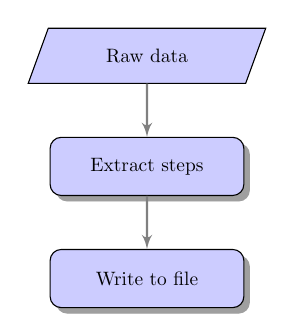
\begin{tikzpicture}[scale=0.7,transform shape]
		
	% Draw diagram elements
	\path \io{1}{Raw data};
		
	\path (p1.south)+(0,-1.5) \etape{2}{Extract steps};
	\path (p2.south)+(0.0,-1.5) \etape{3}{Write to file};
	

	%  \node [below=of p5] (p6-7){};
	
	% Draw arrows between elements
	\path [line] (p1.south) -- node [above]{} (p2);
	\path [line] (p2.south) -- node [above]{} (p3);
	\end{tikzpicture}
	
	\caption[Process of creating data samples]{Process of creating data samples.} \label{fig:createsamples}
\end{figure}
	
\subsubsection{Process of creating samples} \label{sub:createsamples}
	\begin{enumerate}
		\item \textbf{\underline{Raw data}}
		\\
		The dataset is retrieved from the optical force sensor.
		
		\item \textbf{\underline{Extract steps}}
		\\
		Raw data will be partitioned into samples as described in section \ref{subseq:segmentation}.
		
		\item \textbf{\underline{Write to file}}
		\\
		This step will write each data sequence into a file labeled with the terrain name.
		
		
\end{enumerate}
\clearpage

\subsection{Learning process} \label{subsec:learningProc}
When the data samples of each terrain is unified into a single file, the learning process as shown in figure \ref{fig:learningProcess}, is to evaluate each classifier. Rectangles are processes that take a given input and produce an output. The dashed rectangles are processes that can be omitted.
\begin{figure}[h]
	\centering
	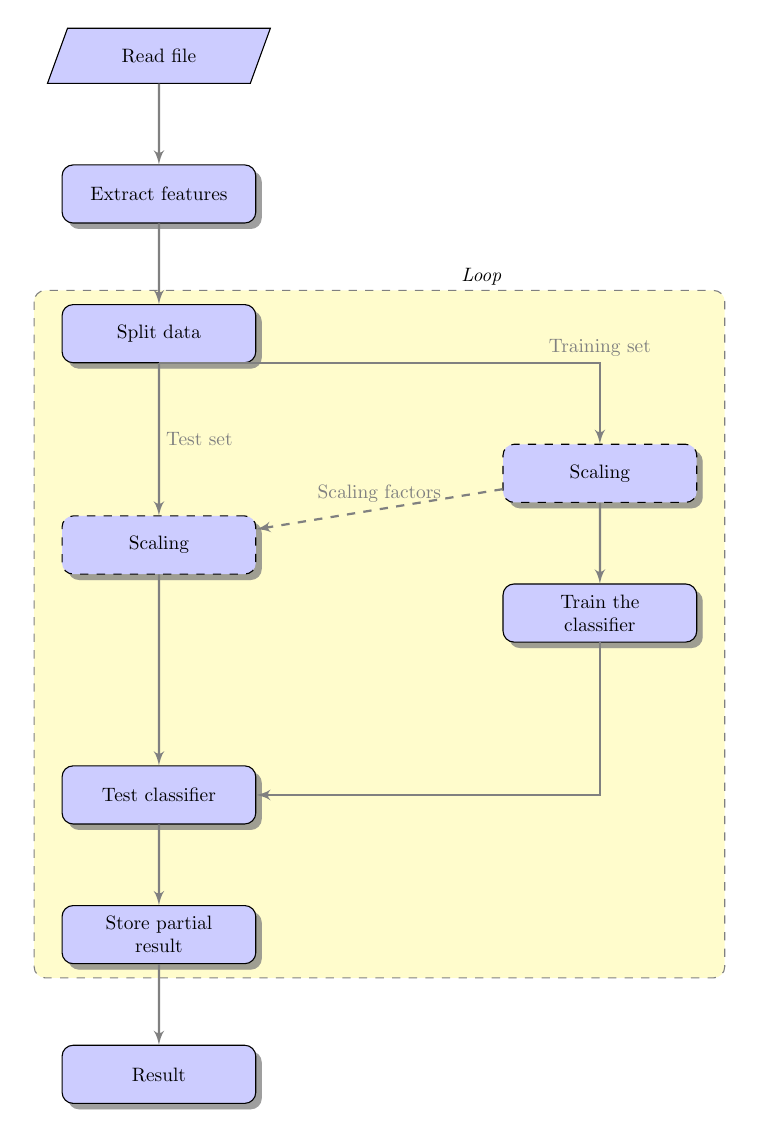
\begin{tikzpicture}[scale=0.7,transform shape]
	
	% Draw diagram elements
	%  \path \io{1}{Raw data};
	\path \io{2}{Read file};
	%  \path (p1.south)+(0,-1.5) \etape{2}{Extract steps};
	\path (p2.south)+(0.0,-2) \etape{3}{Extract features};	
	\path (p3.south)+(0.0,-2) \etape{4}{Split data};
	\path (p4.south)+(8,-2.0) \etapeTo{5}{Scaling};
	\path (p5.south)+(0,-2) \etape{6}{Train the classifier};
	\path (p4.south)+(0,-3.3) \etapeTo{9}{Scaling};
	\path (p9.south)+(0,-4.0) \etape{7}{Test classifier};		
	\path (p7.south)+(0,-2) \etape{10}{Store partial result};
	\path (p10.south)+(0,-2) \etape{8}{Result};
	
	%  \node [below=of p5] (p6-7){};
	
	% Draw arrows between elements
	% \path [line] (p1.south) -- node [above]{} (p2);
	\path [line] (p2.south) -- node [above]{} (p3);
	\path [line] (p3.south) -- node [above]{} (p4);
	\path [line] (p4.south) -| node [above]{Training set} (p5);
	
	\path [line] (p5.south) -- node [above]{} (p6);
	\path [line] (p6.south) |- node [above]{} (p7);
	\path [line] (p4.south) -- node [right]{Test set} (p9);
	\path [line] (p7.south) -- node [above]{} (p10);
	\path [line] (p10.south) -- node [above]{} (p8);
	\path [line] (p9.south) -- node [above]{} (p7);
	%  \path [line] (p5.south) -- node [above]{Feature} (p9);
	\path [line,dashed] (p5) -- node [above]{Scaling factors} (p9);
	\background{p3}{p4}{p5}{p10}{Loop} 
	
	\end{tikzpicture}
	
	\caption[Process of creating and evaluating a certain classifier]{Process of creating and evaluating a certain classifier.} \label{fig:learningProcess}
\end{figure}

\FloatBarrier
	\clearpage
\subsubsection{Details of the learning process} \label{sub:learningprocess}
\begin{enumerate}
\item \textbf{\underline{Read file}}
\\
This step will take a file as input, created from section \ref{sub:createsamples}.
		
\item \textbf{\underline{Extract features}}
\\
This step will create one of the five feature sets as mentioned in section \ref{sec:featuresets}.
		
\item \textbf{\underline{Loop}}
		
\begin{enumerate} 
\item \textbf{\underline{Split data}} \label{en:loop}
\\
The extracted feature vectors are partitioned into training and testing sets. The cross validation is LOOCV, thus the training set consists of 199 samples and one test sample.
			
\item \textbf{\underline{Scaling}}
\\
This step takes the training set as input and standardizes the data as mentioned in section \ref{subsec:scaling}. The scaling factor will be used on the test data.
			
\item \textbf{\underline{Train the classifier}}
\\
The classifier will take the training set as input and train. The parameters of each classifier are default values from Python. 
			
\item \textbf{\underline{Test classifier}} 
\\
This step uses the model to predict the test set.

\item \textbf{\underline{Store partial result}} 
\\
This step will store the partial result of the test sample. If there is still more data to be predicted, it starts from \ref{en:loop}.
\end{enumerate}	
		
\item \textbf{\underline{Result}}
\\
This step will compute the overall results as mentioned in section \ref{subsec:evalclf}, of performance for a certain chosen classifier. 
\end{enumerate}
	
\clearpage
\subsection{Evaluation}
To find the optimal feature combination and algorithm for the optical sensor, the following steps will be investigated:

\begin{enumerate}
	\item Evaluate the performance of all five classifiers with different feature sets. Additionally, investigate whether a feature scaling is appropriate.  
	\item The learning process will be integrated with two different feature selection methods to achieve a better performance. 
	\item \label{it:data} Some of the top performing classifiers along with the feature set will be further tested on new data samples.
	\item Select the two best performers and use a grid search with the training samples to find the best parameters, and test on data samples collected in step \ref{it:data}.
	\item The best performing classifier will be used to evaluate the performance when the robot walks through two different terrains.
	\item Lastly, test whether it is appropriate to use training samples from one sensor to predict the other sensors. 
\end{enumerate}


\chapter{Experiments and results}                     %% ... or ??
This chapter is divided into six main sections, where each of them consists of an experiment. The first section will present the result of each classifier with the different sets of features. The second section will present a modified implementation to increase the performance and its result. The third section will select some of the well performing classifiers with their feature sets to evaluate on a new set of data samples. The fourth section will use a grid search to tune parameters of the two best performing classifiers, and compare to earlier results. The fifth section presents a real time implementation used to evaluate the performance of the best classifier when the robot walks on two different terrains. The last section shows the possibility of using training samples from the sensor mounted on the front left foot of the robot, to predict the front right foot.
 
 
\section{Evaluation of classifier}\label{result_exp1}
This section presents the results of each classifier on different feature sets along with an analysis.
	
\subsection{Results}
Table \ref{exp1} shows the results of each classifier when using the learning approach described in \ref{sub:learningprocess}. The color indicates how high the accuracy is, where green is an accuracy of over 90\%, yellow is between 80\%-89\%, while red is under 79\%. The experiments were done with and without feature scaling.  

\begin{table}[h]
	\centering
	\resizebox{\textwidth}{!}{%
		\begin{tabular}{@{}llll@{}}
			\toprule
			&  & \multicolumn{2}{c}{\textbf{Accuracy}} \\ \cmidrule(l){3-4} 
			\multirow{-2}{*}{\textbf{Feature set}} & \multirow{-2}{*}{\textbf{Classifier}} & \multicolumn{1}{l|}{\textbf{Not scaled}} & \textbf{Scaled} \\ \midrule
			\multicolumn{1}{l|}{} & \multicolumn{1}{l|}{} & \multicolumn{1}{l|}{{\color[HTML]{F8A102} }} & {\color[HTML]{F8A102}} \\
			\multicolumn{1}{l|}{} & \multicolumn{1}{l|}{\multirow{-2}{*}{Bayes Navies}} & \multicolumn{1}{l|}{\multirow{-2}{*}{{\color[HTML]{F8A102} 83\%}}} & \multirow{-2}{*}{{\color[HTML]{F8A102} 83\%}} \\ \cmidrule(l){2-4} 
			\multicolumn{1}{l|}{} & \multicolumn{1}{l|}{Decision tree} & \multicolumn{1}{l|}{{\color[HTML]{009901} 94\%}} & {\color[HTML]{009901} 96\%} \\ \cmidrule(l){2-4} 
			\multicolumn{1}{l|}{} & \multicolumn{1}{l|}{KNN} & \multicolumn{1}{l|}{{\color[HTML]{F8A102} 89\%}} & {\color[HTML]{009901} 91\%} \\ \cmidrule(l){2-4} 
			\multicolumn{1}{l|}{} & \multicolumn{1}{l|}{Neural network} & \multicolumn{1}{l|}{{\color[HTML]{009901} 95\%}} & {\color[HTML]{009901} 96\%} \\ \cmidrule(l){2-4} 
			\multicolumn{1}{l|}{\multirow{-6}{*}{\begin{tabular}[c]{@{}l@{}}Set one -\\ raw data\end{tabular}}} & \multicolumn{1}{l|}{SVM} & \multicolumn{1}{l|}{{\color[HTML]{F8A102} 89\%}} & {\color[HTML]{009901} 93\%} \\ \midrule
			\multicolumn{1}{l|}{} & \multicolumn{1}{l|}{Bayes Navies} & \multicolumn{1}{l|}{{\color[HTML]{F8A102} 82\%}} & {\color[HTML]{F8A102} 82\%} \\ \cmidrule(l){2-4} 
			\multicolumn{1}{l|}{} & \multicolumn{1}{l|}{Decision tree} & \multicolumn{1}{l|}{{\color[HTML]{F8A102} 83\%}} & {\color[HTML]{F8A102} 84\%} \\ \cmidrule(l){2-4} 
			\multicolumn{1}{l|}{} & \multicolumn{1}{l|}{KNN} & \multicolumn{1}{l|}{{\color[HTML]{F8A102} 84\%}} & {\color[HTML]{F8A102} 84\%} \\ \cmidrule(l){2-4} 
			\multicolumn{1}{l|}{} & \multicolumn{1}{l|}{Neural network} & \multicolumn{1}{l|}{{\color[HTML]{F8A102} 83\%}} & {\color[HTML]{F8A102} 88\%} \\ \cmidrule(l){2-4} 
			\multicolumn{1}{l|}{\multirow{-5}{*}{\begin{tabular}[c]{@{}l@{}}Set two - \\ statistical features in \\ time domain\end{tabular}}} & \multicolumn{1}{l|}{SVM} & \multicolumn{1}{l|}{\color[HTML]{FE0000}76\%} & {\color[HTML]{F8A102} 85\%} \\ \midrule
			\multicolumn{1}{l|}{} & \multicolumn{1}{l|}{Bayes Navies} & \multicolumn{1}{l|}{{\color[HTML]{009901} 91\%}} & {\color[HTML]{009901} 91\%} \\ \cmidrule(l){2-4} 
			\multicolumn{1}{l|}{} & \multicolumn{1}{l|}{Decision tree} & \multicolumn{1}{l|}{{\color[HTML]{F8A102} 83\%}} & {\color[HTML]{F8A102} 82\%} \\ \cmidrule(l){2-4} 
			\multicolumn{1}{l|}{} & \multicolumn{1}{l|}{KNN} & \multicolumn{1}{l|}{{\color[HTML]{009901} 91\%}} & {\color[HTML]{F8A102} 88\%} \\ \cmidrule(l){2-4} 
			\multicolumn{1}{l|}{} & \multicolumn{1}{l|}{Neural network} & \multicolumn{1}{l|}{{\color[HTML]{009901} 93\%}} & {\color[HTML]{009901} 93\%} \\ \cmidrule(l){2-4} 
			\multicolumn{1}{l|}{\multirow{-5}{*}{\begin{tabular}[c]{@{}l@{}}Set three - \\ complete frequency \\ domain\end{tabular}}} & \multicolumn{1}{l|}{SVM} & \multicolumn{1}{l|}{\color[HTML]{FE0000}52\%} & {\color[HTML]{009901} 93\%} \\ \midrule
			\multicolumn{1}{l|}{} & \multicolumn{1}{l|}{Bayes Navies} & \multicolumn{1}{l|}{{\color[HTML]{F8A102} 81\%}} & {\color[HTML]{F8A102} 81\%} \\ \cmidrule(l){2-4} 
			\multicolumn{1}{l|}{} & \multicolumn{1}{l|}{Decision tree} & \multicolumn{1}{l|}{{\color[HTML]{F8A102} 80\%}} & {\color[HTML]{F8A102} 82\%} \\ \cmidrule(l){2-4} 
			\multicolumn{1}{l|}{} & \multicolumn{1}{l|}{KNN} & \multicolumn{1}{l|}{{\color[HTML]{F8A102} 88\%}} & {\color[HTML]{F8A102} 84\%} \\ \cmidrule(l){2-4} 
			\multicolumn{1}{l|}{} & \multicolumn{1}{l|}{Neural network} & \multicolumn{1}{l|}{{\color[HTML]{F8A102} 85\%}} & {\color[HTML]{F8A102} 88\%} \\ \cmidrule(l){2-4} 
			\multicolumn{1}{l|}{\multirow{-5}{*}{\begin{tabular}[c]{@{}l@{}}Set four - \\ staticial features in \\ frequency domain\end{tabular}}} & \multicolumn{1}{l|}{SVM} & \multicolumn{1}{l|}{{\color[HTML]{F8A102} 83\%}} & {\color[HTML]{F8A102} 86\%} \\ \midrule
			\multicolumn{1}{l|}{} & \multicolumn{1}{l|}{Bayes Navies} & \multicolumn{1}{l|}{{\color[HTML]{F8A102} 82\%}} & {\color[HTML]{F8A102} 82\%} \\ \cmidrule(l){2-4} 
			\multicolumn{1}{l|}{} & \multicolumn{1}{l|}{Decision tree} & \multicolumn{1}{l|}{\color[HTML]{FE0000}79\%} & {\color[HTML]{F8A102} 80\%} \\ \cmidrule(l){2-4} 
			\multicolumn{1}{l|}{} & \multicolumn{1}{l|}{KNN} & \multicolumn{1}{l|}{{\color[HTML]{F8A102} 88\%}} & {\color[HTML]{F8A102} 84\%} \\ \cmidrule(l){2-4} 
			\multicolumn{1}{l|}{} & \multicolumn{1}{l|}{Neural network} & \multicolumn{1}{l|}{{\color[HTML]{F8A102} 87\%}} & {\color[HTML]{F8A102} 89\%} \\ \cmidrule(l){2-4} 
			\multicolumn{1}{l|}{\multirow{-5}{*}{\begin{tabular}[c]{@{}l@{}}Set five - \\ set 2,4\end{tabular}}} & \multicolumn{1}{l|}{SVM} & \multicolumn{1}{l|}{{\color[HTML]{F8A102} 83\%}} & {\color[HTML]{F8A102} 86\%} \\ \bottomrule
		\end{tabular}%
	}
	\caption[Results from five different feature sets and classifiers without the feature selection method]{Results after following the approach shown in figure \ref{fig:learningProcess}. Green has an accuracy over 90\%, yellow is between 80\%-89\%, while red has accuracy under 79\%.}
	\label{exp1}
\end{table}
\FloatBarrier
	
	
\subsection{Analysis}
All classifiers have an accuracy of at least 70\%. Top performing classifiers are the decision tree and Neural Network with an accuracy of 96\%. However, KNN, Bayes Naives, and SVM also perform well, with an accuracy of 90\%. 
\\
\\
Regarding the feature scaling, out of SVM and KNN which use distances in their computation, SVM had the biggest effect. Feature set three went from 52\% to 93\%. KNN on the other hand was slightly affected by scaling, but mostly gave a lower accuracy. The Neural Network achieved a small improvement, while the decision tree either performed better when scaled or not scaled, dependent on the feature set. Bayes Navies did not undergo any effect by standardized features. Since the feature scaling achieved a big improvement with the SVM and minor improvement on the other classifiers, scaled features will be used in further experiments.
\\
\\
Among the best results are those from either whole raw data sequences or a complete frequency domain where mostly accuracy was over 90\%. While statistics features extracted in either the time domain, frequency domain, or both, gave an accuracy of between 80\% to 89\%.
\\
\\
Besides looking at the performance of each classifier, it is also interesting to look at how data provided from the sensor responds to different terrain. In the time domain, which can be seen in figure \ref{fig:meanxyz}, of the terrains, soft mat differs the most. Forces from floor, carpet and hard mat in the x-direction are relatively similar as shown in figure \ref{fig:meanx}. Forces in the y-direction as seen in figure \ref{fig:meany} are more distinguishable, but the data streams are still quite similar to each other. Meanwhile, forces in the z-direction as seen in figure \ref{fig:meanz} are even more distinguishable. Only carpet and hard mat provide similar forces, but differ in the shapes of curves. Floor and carpet on the other hand, have similar shapes of curves, but differ in the forces. In the frequency domain, again, of the terrains, soft mat differs the most. In contrast to similar data from floor, carpet and hard mat in the time domain, in the frequency domain the floor is more distinguishable as seen in figure \ref{fig:meanxyz}. While the carpet and hard mat are almost equal. However, there is a slight difference between them in the y- and z-direction shown in figures \ref{fig:ffty}, and \ref{fig:fftz} respectively.

\begin{figure} [h]
	\centering
	\begin{subfigure}[b]{0.95\textwidth}
		\includegraphics[width=\textwidth,height=\textheight,keepaspectratio]{Figures/x}
		\caption{Mean of 10 samples in x-direction}
		\label{fig:meanx} 
	\end{subfigure}
	
	\begin{subfigure}[b]{0.95\textwidth}
		\includegraphics[width=\textwidth,height=\textheight,keepaspectratio]{Figures/y}
		\caption{Mean of 10 samples in y-direction}
		\label{fig:meany}
	\end{subfigure}
\end{figure}
\begin{figure}[h] \ContinuedFloat
	\begin{subfigure}[b]{0.95\textwidth}
		\includegraphics[width=\textwidth,height=\textheight,keepaspectratio]{Figures/z}
		\caption{Mean of 10 samples in z-direction}
		\label{fig:meanz}
	\end{subfigure}
	
	\caption[Example of the mean of each terrain for each direction in the time domain]{
		A mean of 10 steps on each terrain in different directions in the
		time domain, where the mean in the x-direction \ref{fig:meanx}, the mean in y-direction \ref{fig:meany},and the mean in z-direction\ref{fig:meanz} are computed}
	\label{fig:meanxyz}
\end{figure}


\begin{figure}[h]
	\centering
	\begin{subfigure}[b]{0.95\textwidth}
		\includegraphics[width=1\linewidth]{Figures/fftx}
		\caption{Mean of 10 samples in x-direction}
		\label{fig:fftx} 
	\end{subfigure}
\end{figure}
\begin{figure}[h] \ContinuedFloat	
	\begin{subfigure}[b]{0.95\textwidth}
		\includegraphics[width=1\linewidth]{Figures/ffty}
		\caption{Mean of 10 samples in y-direction}
		\label{fig:ffty}
	\end{subfigure}
	
	
	\begin{subfigure}[h]{0.95\textwidth}
		\includegraphics[width=1\linewidth]{Figures/fftz}
		\caption{Mean of 10 samples in z-direction}
		\label{fig:fftz}
	\end{subfigure}
	
	\caption[Examples of the mean of each terrain for each direction in the frequency domain]{A mean of 10 steps on each terrain in different directions in the	frequency domain, where the mean in the x-direction \ref{fig:fftx}, the mean in y-direction \ref{fig:ffty},	and the mean in z-direction \ref{fig:fftz} are computed.}
	\label{fig:fftxyz}
\end{figure}
\FloatBarrier

	
	
	
\section{Adding feature selection}
Even though there are classifiers which outperform the others, there is still improvement potential. The result achieved was without a feature selection method. The purpose of not using the feature selection was to investigate the performance without removing any features. However, as mentioned in section \ref{selection}, selecting features from a set can increase the classifier performance and prevent the curse of dimensionality. Thus, in the following experiment, the feature selection will be integrated with the previous implementation described in section \ref{subsec:learningProc} to see if there is any improvement. The modified implementation is shown in figure \ref{fig:approach2}, where the added component is colored as red. The algorithm will select feature on the currently entire data set before the data is partitioned in the cross-validation. The filter and wrapper method will be used, and both are libraries provided by scikit-learn mentioned in section \ref{para:scikit}. The filter method will be removing features with low variance, while the wrapper method is recursive feature elimination and removes features to a desired number. 

\paragraph{Removing features with low variance} \label{ap:variance}
Removing Features with Low Variance (RFLV) is a filter method that removes all features where the variance does not meet some threshold. The default value of the threshold will remove all features that contain the same values, which is unlikely to occur in this experiment. To keep as many feature as possible and at the same time removing features with relative low variance, the threshold will be set to 0.2.

\paragraph{Recursive feature elimination} \label{ap:rfe}
Recursive Feature Elimination (RFE) is a wrapper method that uses a supervised classifier to rank each feature and remove features with a low rank. A chosen estimator will be used to train the set of features, and weigh them. Features with the smallest weights are pruned, and start over to estimate the current remaining set of features. This will be repeated until the desired number of features is reached. In this experiment, the default value will be used, which removes half of the feature set.

	
\begin{figure}[h]
	\centering
	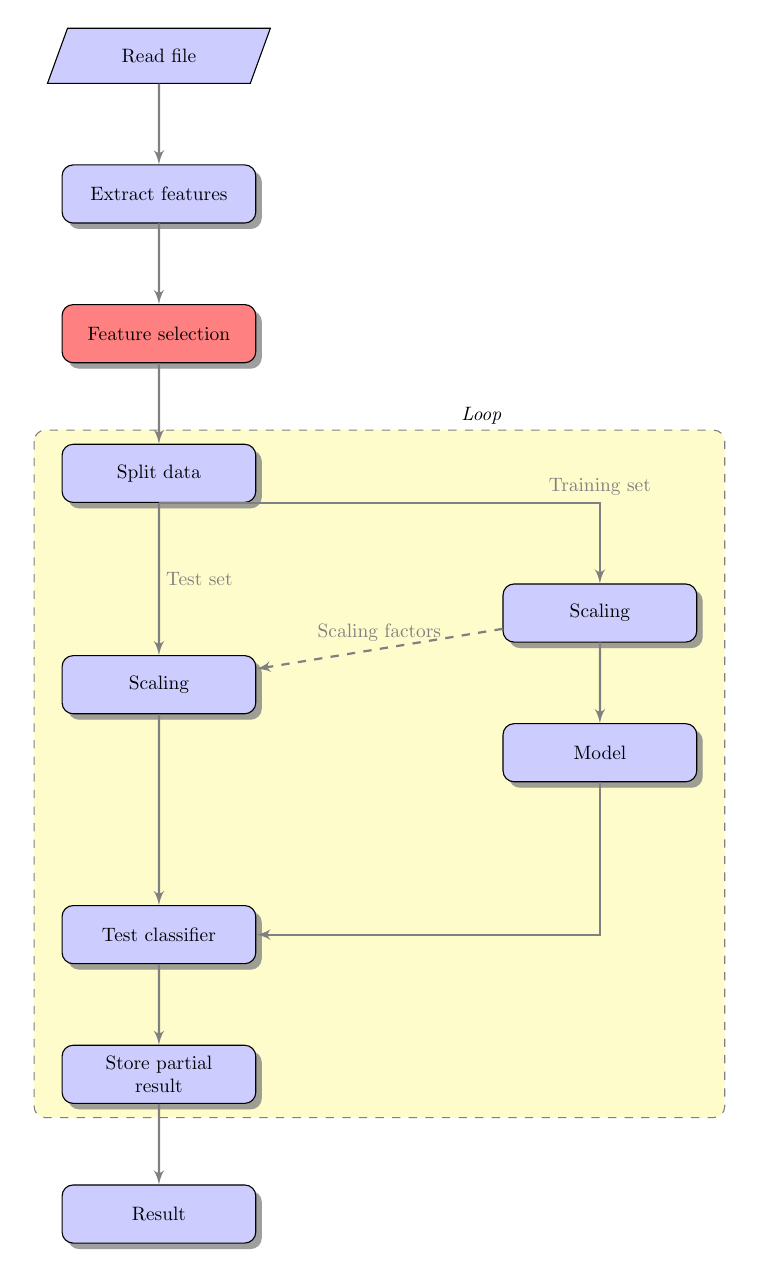
\begin{tikzpicture}[scale=0.7,transform shape]
		
		% Draw diagram elements
		%  \path \io{1}{Raw data};
		\path \io{2}{Read file};
		%  \path (p1.south)+(0,-1.5) \etape{2}{Extract steps};
		\path (p2.south)+(0.0,-2) \etape{3}{Extract features};
		\path (p3.south)+(0.0,-2) \etapeTre{11}{Feature selection};
		
		\path (p11.south)+(0.0,-2) \etape{4}{Split data};
		\path (p4.south)+(8,-2.0) \etape{5}{Scaling};
		\path (p5.south)+(0,-2) \etape{6}{Model};
		\path (p4.south)+(0,-3.3) \etape{9}{Scaling};
		\path (p9.south)+(0,-4.0) \etape{7}{Test classifier};		
		\path (p7.south)+(0,-2) \etape{10}{Store partial result};
		\path (p10.south)+(0,-2) \etape{8}{Result};
		
		%  \node [below=of p5] (p6-7) {};
		
		% Draw arrows between elements
		% \path [line] (p1.south) -- node [above] {} (p2);
		\path [line] (p2.south) -- node [above]{} (p3);
		\path [line] (p3.south) -- node [above]{} (p11);
		\path [line] (p11.south) -- node [above]{} (p4);
		\path [line] (p4.south) -| node [above]{Training set} (p5);
		
		\path [line] (p5.south) -- node [above]{} (p6);
		\path [line] (p6.south) |- node [above]{} (p7);
		\path [line] (p4.south) -- node [right]{Test set} (p9);
		\path [line] (p7.south) -- node [above]{} (p10);
		\path [line] (p10.south) -- node [above]{} (p8);
		\path [line] (p9.south) -- node [above]{} (p7);
		%  \path [line] (p5.south) -- node [above]{Feature} (p9);
		\path [line,dashed] (p5) -- node [above]{Scaling factors} (p9);
		\background{p3}{p4}{p5}{p10}{Loop} 
		
		\end{tikzpicture}
		
		\caption[Evaluation process with feature selection]{Modified evaluation process from \ref{subsec:learningProc}, where the new function is feature selection and is colored red.} 
		\label{fig:approach2}
	\end{figure}
\FloatBarrier
\newpage
\subsection{Results}
Table \ref{tab:exp2_1} shows the new number of features after they were removed for each feature set, and table \ref{tab:exp2} shows the results for when feature selection is applied to the earlier learning approach and is compared to previous implementation. The five highest performing models are marked with bold text and will be used in further experiments.

\begin{table}[h]
	\centering
	\begin{tabular}{llll}
		\hline
		\textbf{Feature set} & \textbf{Old} & \textbf{Filter} & \textbf{Wrapper} \\ \hline
		Set 1 & 375 & 230 & 187 \\
		Set 2 & 21 & 8 & 10 \\
		Set 3 & 183 & 2 & 91 \\
		Set 4 & 24 & 11 & 12 \\
		Set 5 & 45 & 19 & 22 \\ \hline
	\end{tabular}
	\caption[Results of lengths of feature vector after the feature selection method]{New length of each feature set after applying the feature selection method.}
	\label{tab:exp2_1}
\end{table}
\FloatBarrier


\begin{table}[h]
	\centering
	\resizebox{\textwidth}{!} & \multicolumn{1}{l|}{{\color[HTML]{FE0000} 78\%}} & {\color[HTML]{FE0000} 81\%} \\ \cmidrule(l){2-5} 
			\multicolumn{1}{l|}{} & \multicolumn{1}{l|}{\textbf{Decision tree}} & \multicolumn{1}{l|}{\textbf{96\%}} & \multicolumn{1}{l|}{\color[HTML]{F8A102}\textbf{96\%}} & {\color[HTML]{FE0000} 93\%} \\ \cmidrule(l){2-5} 
			\multicolumn{1}{l|}{} & \multicolumn{1}{l|}{KNN} & \multicolumn{1}{l|}{91\%} & \multicolumn{1}{l|}{{\color[HTML]{009901} 95\%}} & {\color[HTML]{009901} 93\%} \\ \cmidrule(l){2-5} 
			\multicolumn{1}{l|}{} & \multicolumn{1}{l|}{\textbf{Neural network}} & \multicolumn{1}{l|}{\textbf{96\%}} & \multicolumn{1}{l|}{{\color[HTML]{FE0000} 94\%}} & {\color[HTML]{FE0000} 95\%} \\ \cmidrule(l){2-5} 
			\multicolumn{1}{l|}{\multirow{-5}{*}{\textbf{\begin{tabular}[c]{@{}l@{}}Set one -\\ raw data\end{tabular}}}} & \multicolumn{1}{l|}{SVM} & \multicolumn{1}{l|}{93\%} & \multicolumn{1}{l|}{{\color[HTML]{FE0000} 91\%}} & {\color[HTML]{009901} 94\%} \\ \midrule
			\multicolumn{1}{l|}{} & \multicolumn{1}{l|}{Bayes Navies} & \multicolumn{1}{l|}{82\%} & \multicolumn{1}{l|}{{\color[HTML]{FE0000} 74\%}} & {\color[HTML]{009901} 84\%} \\ \cmidrule(l){2-5} 
			\multicolumn{1}{l|}{} & \multicolumn{1}{l|}{Decision tree} & \multicolumn{1}{l|}{84\%} & \multicolumn{1}{l|}{{\color[HTML]{FE0000} 79\%}} & {\color[HTML]{FE0000} 81\%} \\ \cmidrule(l){2-5} 
			\multicolumn{1}{l|}{} & \multicolumn{1}{l|}{KNN} & \multicolumn{1}{l|}{84\%} & \multicolumn{1}{l|}{{\color[HTML]{FE0000} 82\%}} & {\color[HTML]{FE0000} 82\%} \\ \cmidrule(l){2-5} 
			\multicolumn{1}{l|}{} & \multicolumn{1}{l|}{Neural network} & \multicolumn{1}{l|}{88\%} & \multicolumn{1}{l|}{{\color[HTML]{FE0000} 81\%}} & {\color[HTML]{FE0000} 84\%} \\ \cmidrule(l){2-5} 
			\multicolumn{1}{l|}{\multirow{-5}{*}{\begin{tabular}[c]{@{}l@{}}Set two - \\ statistical features in \\ time domain\end{tabular}}} & \multicolumn{1}{l|}{SVM} & \multicolumn{1}{l|}{85\%} & \multicolumn{1}{l|}{{\color[HTML]{FE0000} 80\%}} & {\color[HTML]{FE0000} 83\%} \\ \midrule
			\multicolumn{1}{l|}{} & \multicolumn{1}{l|}{Bayes Navies} & \multicolumn{1}{l|}{91\%} & \multicolumn{1}{l|}{{\color[HTML]{FE0000} 76\%}} & {\color[HTML]{009901} 94\%} \\ \cmidrule(l){2-5} 
			\multicolumn{1}{l|}{} & \multicolumn{1}{l|}{Decision tree} & \multicolumn{1}{l|}{82\%} & \multicolumn{1}{l|}{{\color[HTML]{FE0000} 76\%}} & {\color[HTML]{FE0000} 81\%} \\ \cmidrule(l){2-5} 
			\multicolumn{1}{l|}{} & \multicolumn{1}{l|}{KNN} & \multicolumn{1}{l|}{88\%} & \multicolumn{1}{l|}{{\color[HTML]{FE0000} 83\%}} & \color[HTML]{F8A102} 88\% \\ \cmidrule(l){2-5} 
			\multicolumn{1}{l|}{} & \multicolumn{1}{l|}{Neural network} & \multicolumn{1}{l|}{93\%} & \multicolumn{1}{l|}{{\color[HTML]{FE0000} 78\%}} & {\color[HTML]{009901} 94\%} \\ \cmidrule(l){2-5} 
			\multicolumn{1}{l|}{\multirow{-5}{*}{\textbf{\begin{tabular}[c]{@{}l@{}}Set three - \\ complete frequency \\ domain\end{tabular}}}} & \multicolumn{1}{l|}{\textbf{SVM}} & \multicolumn{1}{l|}{93\%} & \multicolumn{1}{l|}{{\color[HTML]{FE0000} 79\%}} & {\color[HTML]{009901} \textbf{97\%}} \\ \midrule
			\multicolumn{1}{l|}{} & \multicolumn{1}{l|}{Bayes Navies} & \multicolumn{1}{l|}{81\%} & \multicolumn{1}{l|}{{\color[HTML]{FE0000} 75\%}} & {\color[HTML]{FE0000} 79\%} \\ \cmidrule(l){2-5} 
			\multicolumn{1}{l|}{} & \multicolumn{1}{l|}{Decision tree} & \multicolumn{1}{l|}{82\%} & \multicolumn{1}{l|}{\color[HTML]{F8A102} 82\%} & {\color[HTML]{FE0000} 81\%} \\ \cmidrule(l){2-5} 
			\multicolumn{1}{l|}{} & \multicolumn{1}{l|}{KNN} & \multicolumn{1}{l|}{84\%} & \multicolumn{1}{l|}{{\color[HTML]{009901} 85\%}} & {\color[HTML]{009901} 86\%} \\ \cmidrule(l){2-5} 
			\multicolumn{1}{l|}{} & \multicolumn{1}{l|}{Neural network} & \multicolumn{1}{l|}{88\%} & \multicolumn{1}{l|}{{\color[HTML]{FE0000} 84\%}} & {\color[HTML]{009901} 90\%} \\ \cmidrule(l){2-5} 
			\multicolumn{1}{l|}{\multirow{-5}{*}{\begin{tabular}[c]{@{}l@{}}Set four - \\ staticial features in \\ frequency domain\end{tabular}}} & \multicolumn{1}{l|}{SVM} & \multicolumn{1}{l|}{86\%} & \multicolumn{1}{l|}{{\color[HTML]{FE0000} 82\%}} & {\color[HTML]{009901} 86\%} \\ \midrule
			\multicolumn{1}{l|}{} & \multicolumn{1}{l|}{Bayes Navies} & \multicolumn{1}{l|}{82\%} & \multicolumn{1}{l|}{{\color[HTML]{FE0000} 74\%}} & {\color[HTML]{009901} 84\%} \\ \cmidrule(l){2-5} 
			\multicolumn{1}{l|}{} & \multicolumn{1}{l|}{Decision tree} & \multicolumn{1}{l|}{80\%} & \multicolumn{1}{l|}{{\color[HTML]{009901} 82\%}} & {\color[HTML]{009901} 82\%} \\ \cmidrule(l){2-5} 
			\multicolumn{1}{l|}{} & \multicolumn{1}{l|}{KNN} & \multicolumn{1}{l|}{84\%} & \multicolumn{1}{l|}{{\color[HTML]{009901} 86\%}} & {\color[HTML]{009901} 86\%} \\ \cmidrule(l){2-5} 
			\multicolumn{1}{l|}{} & \multicolumn{1}{l|}{\textbf{Neural network}} & \multicolumn{1}{l|}{\textbf{89\%}} & \multicolumn{1}{l|}{{\color[HTML]{FE0000} 81\%}} & {\color[HTML]{FE0000} 85\%} \\ \cmidrule(l){2-5} 
			\multicolumn{1}{l|}{\multirow{-5}{*}{\textbf{\begin{tabular}[c]{@{}l@{}}Set five - \\ set 2,4\end{tabular}}}} & \multicolumn{1}{l|}{SVM} & \multicolumn{1}{l|}{86\%} & \multicolumn{1}{l|}{{\color[HTML]{FE0000} 83\%}} & {\color[HTML]{009901} 84\%} \\ \bottomrule
		\end{tabular}%
	}
	\caption[Results from five different feature sets and classifiers with the feature selection method]{Results from five different feature sets and classifiers when applying the feature selection method.}
	\label{tab:exp2}
\end{table}
\FloatBarrier
	
\subsection{Analysis}
Adding the feature selection has decreased performance of most classifiers. The filter method with feature set three gave the poorest performance. This is also the set which had the most features removed, as seen in table \ref{tab:exp2_1}. However, the sets that contain statistical metrics have been removed to nearly equal length for both methods, and they generally have achieved approximately the same results. The wrapper selection also has some classifiers that performed less accurately, but the decreased accuracy is less than the filter method. However, SVM with feature set three has improved significantly with an accuracy of 97\%.
\\
\\
It will be interesting to investigate the features selected from each method. However, this thesis will only present features which gave the highest accuracy, that is the wrapper on feature set three. Other selected features can be seen in appendix \ref{ap:self}. To give a more reliable comparison between each feature on each terrain, the figure in \ref{fig:wrapperset5} is the mean of ten steps on each terrain in the frequency domain. The first feature in the x, y, and z-directions is the feature that shows most differences among them. Further behind in the feature set, each feature becomes more equal. Generally, the soft mat differs the most among the terrains, while the floor, carpet, and hard mat may show differences, but tend to overlap each other.


\begin{figure} [h]
	\centering
	\begin{subfigure}[b]{\textwidth}
		\includegraphics[width=\textwidth,height=\textheight,keepaspectratio]{Figures/featureselx}
		\caption{Features in x-direction}
		\label{fig:featurex} 
	\end{subfigure}
	
	\begin{subfigure}[b]{\textwidth}
		\includegraphics[width=\textwidth,height=\textheight,keepaspectratio]{Figures/featuresely}
		\caption{Features in y-direction}
		\label{fig:featurey}
	\end{subfigure}
	
	\begin{subfigure}[h]{\textwidth}
		\includegraphics[width=\textwidth,height=\textheight,keepaspectratio]{Figures/featureselz}
		\caption{Features in z-direction}
		\label{fig:featurez}
	\end{subfigure}

	\caption[Comparison of each feature on different terrains selected from RFE]{A comparison of each feature selected by RFE, for each terrain on feature set three.}
	\label{fig:wrapperset5}
\end{figure}
\FloatBarrier

\section{Cross validation with unseen data} \label{seq:crossunseen}
Note that the k-fold validation in earlier experiments were only using the same single set both for training and testing, which make the data referring to themselves and has the risk of not generalizing the classifier. In this case, results achieved from table \ref{exp1} and table \ref{tab:exp2} only give an estimation on how successful a classifier is, but does not tell how well it predicts on unseen data. One way to avoid this issue is to make the training and testing sets independent of each other, so the predictions will be based on new and unseen data \cite{26b23e912c654fe4b7478fd910130195}. The following experiment will be using high performing classifiers which are shown in table \ref{tab:exp2}, marked with bold text. As there are three shared second-best classifiers, all of them will be included in this experiment. Additionally, the Neural Network without a selection method with feature set five achieved a satisfying result which will also be further investigated. The reason is that the four best performing classifiers only use either the entire raw data or frequency domain. Thus, it will be interesting to compare a classifier that uses statistical features as well.
\\
\\
In this experiment 50 new samples for each terrain is collected. The cross validation will use the old dataset as a training set, while the newly collected samples will be used as a test set. The cross validation technique in this experiment is still LOOCV, in order to train as many samples as possible. To achieve a reliable performance estimation, it can be done by running the cross-validation multiple times \cite{Refaeilzadeh2009}. Thus, the training and test sets will be randomly shuffled before each round of cross validation, and each classifier will be run five times. The table \ref{tab:exp4} shows the classifier and feature set used in this experiment.

\begin{table}[h]
	\centering
	\begin{tabular}{@{}lll@{}}
		\toprule
		\textbf{Classifier} & \textbf{\begin{tabular}[c]{@{}l@{}}Feature\\ set\end{tabular}} & \textbf{\begin{tabular}[c]{@{}l@{}}Feature\\ selection\end{tabular}} \\ \midrule
		SVM & 3 & RFE \\
		Neural network & 1 & None \\
		Neural network & 5 & None \\
		Decision tree & 1 & None \\
		Decision tree & 1 & \begin{tabular}[c]{@{}l@{}}Removing features \\ with low variance\end{tabular} \\ \bottomrule
	\end{tabular}
	\caption[Overview of top performing models tested on unseen data samples]{Overview of top performing classifiers with their feature set which will be used to test on unseen data.}
	\label{tab:exp4}
\end{table}
\FloatBarrier
\newpage
\subsection{Results}
An overview of the performance of the five top performed classifier is shown as a box plot in figure \ref{fig:boxexp}. Again, the top performing is the SVM, and second best is the Neural network with feature set five, and these will be used in further experiments. The other classifiers have heavily decreased their accuracy in their performance.

\begin{figure}[h]
	\centering
	\includegraphics[width=\textwidth,height=\textheight,keepaspectratio]{Figures/compareUnseen}
	\caption[Boxplot of the five top performing classifiers]{Boxplot of the five top performing classifiers on unseen data.}
	\label{fig:boxexp}
\end{figure}
\FloatBarrier
\subsection{Analysis}
This section will present a more detailed description of each classifiers performance with statistics metrics mentioned in section \ref{subsec:evalclf}. The following paragraphs are organized by average accuracy in descending order.
\newpage

\subsubsection{SVM - feature set three - RFE} \label{sb:svmwrapper}
This is the best performing classifier and table \ref{svmexp} shows the accuracy of each run. The average performance of predicting unseen data has an accuracy of 94.8\%, and compared to the old result from \ref{tab:exp2} it has decreased by 2.2\%. The classifier easily predicts floor, carpet, and soft mat, while it has some difficulties predicting hard mat. When the robot is on hard mat it has an average precision of 84\%, and it tends to predict it as carpet. Because the hard mat tends to be predicted as other terrains, the f-score for floor and carpet is decreased a little as seen in table \ref{fscoresvm}. The hard mat and carpet have relative equal f-scores. However, the carpet got a lower recall, but higher precision, while the hard mat got higher recall, but lower precision.

\begin{table}[h]
	\begin{subtable}[h]{1\textwidth}
		\centering
		\captionsetup{justification=centering}
		\begin{tabular}{@{}llllll@{}}
			\toprule
			\multirow{2}{*}{\textbf{Terrain}} & \multicolumn{5}{c}{\textbf{Run}} \\ \cmidrule(l){2-6} 
			& \multicolumn{1}{l|}{\textbf{1}} & \multicolumn{1}{l|}{\textbf{2}} & \multicolumn{1}{l|}{\textbf{3}} & \multicolumn{1}{l|}{\textbf{4}} & \textbf{5} \\ \midrule
			\multicolumn{1}{l|}{Floor} & \multicolumn{1}{l|}{100\%} & \multicolumn{1}{l|}{100\%} & \multicolumn{1}{l|}{100\%} & \multicolumn{1}{l|}{100\%} & 100\% \\ \midrule
			\multicolumn{1}{l|}{Carpet} & \multicolumn{1}{l|}{94\%} & \multicolumn{1}{l|}{96\%} & \multicolumn{1}{l|}{96\%} & \multicolumn{1}{l|}{96\%} & 98\% \\ \midrule
			\multicolumn{1}{l|}{Soft mat} & \multicolumn{1}{l|}{100\%} & \multicolumn{1}{l|}{100\%} & \multicolumn{1}{l|}{100\%} & \multicolumn{1}{l|}{100\%} & 100\% \\ \midrule
			\multicolumn{1}{l|}{Hard mat} & \multicolumn{1}{l|}{82\%} & \multicolumn{1}{l|}{94\%} & \multicolumn{1}{l|}{82\%} & \multicolumn{1}{l|}{80\%} & 82\% \\ \bottomrule
		\end{tabular}
		\caption{Precision of SVM - RFE - feature set three}
		\label{pressvm}
	\end{subtable}
\end{table}

	\begin{table}[h]\ContinuedFloat
	\begin{subtable}[h]{1\textwidth}
		\centering
		\captionsetup{justification=centering}
		\begin{tabular}{@{}llllll@{}}
			\toprule
			\multirow{2}{*}{\textbf{Terrain}} & \multicolumn{5}{c}{\textbf{Run}} \\ \cmidrule(l){2-6} 
			& \multicolumn{1}{l|}{\textbf{1}} & \multicolumn{1}{l|}{\textbf{2}} & \multicolumn{1}{l|}{\textbf{3}} & \multicolumn{1}{l|}{\textbf{4}} & \textbf{5} \\ \midrule
			\multicolumn{1}{l|}{Floor} & \multicolumn{1}{l|}{90.9\%} & \multicolumn{1}{l|}{92.6\%} & \multicolumn{1}{l|}{92.6\%} & \multicolumn{1}{l|}{92.6\%} & 87.5\% \\ \midrule
			\multicolumn{1}{l|}{Carpet} & \multicolumn{1}{l|}{87\%} & \multicolumn{1}{l|}{98\%} & \multicolumn{1}{l|}{87.2\%} & \multicolumn{1}{l|}{85.7\%} & 98\% \\ \midrule
			\multicolumn{1}{l|}{Soft mat} & \multicolumn{1}{l|}{100\%} & \multicolumn{1}{l|}{100\%} & \multicolumn{1}{l|}{100\%} & \multicolumn{1}{l|}{100\%} & 100\% \\ \midrule
			\multicolumn{1}{l|}{Hard mat} & \multicolumn{1}{l|}{100\%} & \multicolumn{1}{l|}{100\%} & \multicolumn{1}{l|}{100\%} & \multicolumn{1}{l|}{100\%} & 100\% \\ \bottomrule
		\end{tabular}
		\caption{Recall of SVM - RFE - feature set three}
		\label{recallsvm}
	\end{subtable}
\end{table}
\begin{table}[h]\ContinuedFloat
	\begin{subtable}[h]{1\textwidth}
		\centering
		\captionsetup{justification=centering}
		\begin{tabular}{@{}llllll@{}}
			\toprule
			\multirow{2}{*}{\textbf{Terrain}} & \multicolumn{5}{c}{\textbf{Run}} \\ \cmidrule(l){2-6} 
			& \multicolumn{1}{l|}{\textbf{1}} & \multicolumn{1}{l|}{\textbf{2}} & \multicolumn{1}{l|}{\textbf{3}} & \multicolumn{1}{l|}{\textbf{4}} & \textbf{5} \\ \midrule
			\multicolumn{1}{l|}{Floor} & \multicolumn{1}{l|}{95.2\%} & \multicolumn{1}{l|}{96.2\%} & \multicolumn{1}{l|}{96.2\%} & \multicolumn{1}{l|}{96.2\%} & 98\% \\ \midrule
			\multicolumn{1}{l|}{Carpet} & \multicolumn{1}{l|}{90.4\%} & \multicolumn{1}{l|}{97\%} & \multicolumn{1}{l|}{91.4\%} & \multicolumn{1}{l|}{90.6\%} & 97\% \\ \midrule
			\multicolumn{1}{l|}{Soft mat} & \multicolumn{1}{l|}{100\%} & \multicolumn{1}{l|}{100\%} & \multicolumn{1}{l|}{100\%} & \multicolumn{1}{l|}{100\%} & 100\% \\ \midrule
			\multicolumn{1}{l|}{Hard mat} & \multicolumn{1}{l|}{90.1\%} & \multicolumn{1}{l|}{96.9\%} & \multicolumn{1}{l|}{90.1\%} & \multicolumn{1}{l|}{88\%} & 90.1\% \\ \bottomrule
		\end{tabular}
		\caption{F-score of SVM - RFE - feature set three}
		\label{fscoresvm}
	\end{subtable}
\end{table}

\begin{table}[h]\ContinuedFloat
	\begin{subtable}[h]{1\textwidth} 
		\centering
		\captionsetup{justification=centering}
		\begin{tabular}{@{}llllll@{}}
			\toprule
			\multirow{2}{*}{\textbf{Run}} & \multirow{2}{*}{\textbf{Accuracy}} & \multicolumn{4}{c}{\textbf{Confusion matrix}} \\ \cmidrule(l){3-6} 
			&  & \multicolumn{1}{l|}{\textbf{Floor}} & \multicolumn{1}{l|}{\textbf{Carpet}} & \multicolumn{1}{l|}{\textbf{Soft mat}} & \textbf{Hard mat} \\ \midrule
			\multicolumn{1}{l|}{\multirow{4}{*}{1}} & \multicolumn{1}{l|}{\multirow{4}{*}{94\%}} & \multicolumn{1}{l|}{50} & \multicolumn{1}{l|}{0} & \multicolumn{1}{l|}{0} & 0 \\ \cmidrule(l){3-6} 
			\multicolumn{1}{l|}{} & \multicolumn{1}{l|}{} & \multicolumn{1}{l|}{3} & \multicolumn{1}{l|}{47} & \multicolumn{1}{l|}{0} & 0 \\ \cmidrule(l){3-6} 
			\multicolumn{1}{l|}{} & \multicolumn{1}{l|}{} & \multicolumn{1}{l|}{0} & \multicolumn{1}{l|}{0} & \multicolumn{1}{l|}{50} & 0 \\ \cmidrule(l){3-6} 
			\multicolumn{1}{l|}{} & \multicolumn{1}{l|}{} & \multicolumn{1}{l|}{2} & \multicolumn{1}{l|}{7} & \multicolumn{1}{l|}{0} & 41 \\ \midrule
			\multicolumn{1}{l|}{\multirow{4}{*}{2}} & \multicolumn{1}{l|}{\multirow{4}{*}{97\%}} & \multicolumn{1}{l|}{50} & \multicolumn{1}{l|}{0} & \multicolumn{1}{l|}{0} & 0 \\ \cmidrule(l){3-6} 
			\multicolumn{1}{l|}{} & \multicolumn{1}{l|}{} & \multicolumn{1}{l|}{2} & \multicolumn{1}{l|}{48} & \multicolumn{1}{l|}{0} & 0 \\ \cmidrule(l){3-6} 
			\multicolumn{1}{l|}{} & \multicolumn{1}{l|}{} & \multicolumn{1}{l|}{0} & \multicolumn{1}{l|}{0} & \multicolumn{1}{l|}{50} & 0 \\ \cmidrule(l){3-6} 
			\multicolumn{1}{l|}{} & \multicolumn{1}{l|}{} & \multicolumn{1}{l|}{2} & \multicolumn{1}{l|}{1} & \multicolumn{1}{l|}{0} & 47 \\ \midrule
			\multicolumn{1}{l|}{\multirow{4}{*}{3}} & \multicolumn{1}{l|}{\multirow{4}{*}{94\%}} & \multicolumn{1}{l|}{50} & \multicolumn{1}{l|}{0} & \multicolumn{1}{l|}{0} & 0 \\ \cmidrule(l){3-6} 
			\multicolumn{1}{l|}{} & \multicolumn{1}{l|}{} & \multicolumn{1}{l|}{2} & \multicolumn{1}{l|}{48} & \multicolumn{1}{l|}{0} & 0 \\ \cmidrule(l){3-6} 
			\multicolumn{1}{l|}{} & \multicolumn{1}{l|}{} & \multicolumn{1}{l|}{0} & \multicolumn{1}{l|}{0} & \multicolumn{1}{l|}{50} & 0 \\ \cmidrule(l){3-6} 
			\multicolumn{1}{l|}{} & \multicolumn{1}{l|}{} & \multicolumn{1}{l|}{2} & \multicolumn{1}{l|}{7} & \multicolumn{1}{l|}{0} & 41 \\ \midrule
			\multicolumn{1}{l|}{\multirow{4}{*}{4}} & \multicolumn{1}{l|}{\multirow{4}{*}{94\%}} & \multicolumn{1}{l|}{50} & \multicolumn{1}{l|}{0} & \multicolumn{1}{l|}{0} & 0 \\ \cmidrule(l){3-6} 
			\multicolumn{1}{l|}{} & \multicolumn{1}{l|}{} & \multicolumn{1}{l|}{2} & \multicolumn{1}{l|}{48} & \multicolumn{1}{l|}{0} & 0 \\ \cmidrule(l){3-6} 
			\multicolumn{1}{l|}{} & \multicolumn{1}{l|}{} & \multicolumn{1}{l|}{0} & \multicolumn{1}{l|}{0} & \multicolumn{1}{l|}{50} & 0 \\ \cmidrule(l){3-6} 
			\multicolumn{1}{l|}{} & \multicolumn{1}{l|}{} & \multicolumn{1}{l|}{2} & \multicolumn{1}{l|}{8} & \multicolumn{1}{l|}{0} & 40 \\ \midrule
			\multicolumn{1}{l|}{\multirow{4}{*}{5}} & \multicolumn{1}{l|}{\multirow{4}{*}{95\%}} & \multicolumn{1}{l|}{50} & \multicolumn{1}{l|}{0} & \multicolumn{1}{l|}{0} & 0 \\ \cmidrule(l){3-6} 
			\multicolumn{1}{l|}{} & \multicolumn{1}{l|}{} & \multicolumn{1}{l|}{1} & \multicolumn{1}{l|}{49} & \multicolumn{1}{l|}{0} & 0 \\ \cmidrule(l){3-6} 
			\multicolumn{1}{l|}{} & \multicolumn{1}{l|}{} & \multicolumn{1}{l|}{0} & \multicolumn{1}{l|}{0} & \multicolumn{1}{l|}{50} & 0 \\ \cmidrule(l){3-6} 
			\multicolumn{1}{l|}{} & \multicolumn{1}{l|}{} & \multicolumn{1}{l|}{2} & \multicolumn{1}{l|}{7} & \multicolumn{1}{l|}{0} & 41 \\ \bottomrule
		\end{tabular}
		\caption{Accuracy and confusion matrix for SVM with a wrapper using feature set three after five runs. Regarding the confusion matrix, the rows show the actual terrains and the columns show the predicted terrains.}
		\label{subt:svmexp}
	\end{subtable}
	\caption[Results of SVM on feature set three with RFE]{Results of SVM with RFE on feature set three after five trials, with precision \ref{pressvm}, recall \ref{recallsvm}, f-score \ref{fscoresvm}, and accuracy and confusion matrix \ref{subt:svmexp}.}
	\label{svmexp}
\end{table}
\FloatBarrier
\newpage
\subsubsection{Neural network - feature set five}
This is the second best performing classifier and the table shows the accuracy of each run. The average performance of predicting unseen data has an accuracy of 78.2\%, and compared to the old result from \ref{tab:exp2} it has decreased by 10.8\%. The classifier has difficulties predicting the hard mat, and tends to predict it as carpet. Soft mat is the easiest to identify, but there is a minor amount of error in the recall when the robot is on the floor. The floor has the second highest accuracy with over 80\%. It has a precision of at least 88\%, and the recall is under 80\%, because there is shown misclassification of floor when the robot is on hard mat and floor. The carpet has a precision of at least 78\%, but the recall is under 63.5\%, while the hard mat has a higher recall of at least 71\%, and lower precision of approximately 41\%.


\begin{table}[h]
	\begin{subtable}[h]{1\textwidth}
		\centering
		\captionsetup{justification=centering}
		\begin{tabular}{@{}llllll@{}}
			\toprule
			\multirow{2}{*}{\textbf{Terrain}} & \multicolumn{5}{c}{\textbf{Run}} \\ \cmidrule(l){2-6} 
			& \multicolumn{1}{l|}{\textbf{1}} & \multicolumn{1}{l|}{\textbf{2}} & \multicolumn{1}{l|}{\textbf{3}} & \multicolumn{1}{l|}{\textbf{4}} & \textbf{5} \\ \midrule
			\multicolumn{1}{l|}{Floor} & \multicolumn{1}{l|}{96\%} & \multicolumn{1}{l|}{92\%} & \multicolumn{1}{l|}{88\%} & \multicolumn{1}{l|}{90\%} & 94\% \\ \midrule
			\multicolumn{1}{l|}{Carpet} & \multicolumn{1}{l|}{80\%} & \multicolumn{1}{l|}{78\%} & \multicolumn{1}{l|}{84\%} & \multicolumn{1}{l|}{78\%} & 80\% \\ \midrule
			\multicolumn{1}{l|}{Soft mat} & \multicolumn{1}{l|}{100\%} & \multicolumn{1}{l|}{100\%} & \multicolumn{1}{l|}{100\%} & \multicolumn{1}{l|}{100\%} & 100\% \\ \midrule
			\multicolumn{1}{l|}{Hard mat} & \multicolumn{1}{l|}{40\%} & \multicolumn{1}{l|}{40\%} & \multicolumn{1}{l|}{42\%} & \multicolumn{1}{l|}{40\%} & 42\% \\ \bottomrule
		\end{tabular}
		\caption{Precision - neural network - feature set five.}
		\label{tabl:nnset5pre}
	\end{subtable}
%\end{table}
\\
\\
\\
%\begin{table}[h]\ContinuedFloat
	\begin{subtable}[h]{1\textwidth}
		\centering
		\captionsetup{justification=centering}
		\begin{tabular}{@{}llllll@{}}
			\toprule
			\multirow{2}{*}{\textbf{Terrain}} & \multicolumn{5}{c}{\textbf{Run}} \\ \cmidrule(l){2-6} 
			& \multicolumn{1}{l|}{\textbf{1}} & \multicolumn{1}{l|}{\textbf{2}} & \multicolumn{1}{l|}{\textbf{3}} & \multicolumn{1}{l|}{\textbf{4}} & \textbf{5} \\ \midrule
			\multicolumn{1}{l|}{Floor} & \multicolumn{1}{l|}{78.7\%} & \multicolumn{1}{l|}{79.3\%} & \multicolumn{1}{l|}{80\%} & \multicolumn{1}{l|}{76.3\%} & 78.3\% \\ \midrule
			\multicolumn{1}{l|}{Carpet} & \multicolumn{1}{l|}{63.5\%} & \multicolumn{1}{l|}{60.9\%} & \multicolumn{1}{l|}{63.6\%} & \multicolumn{1}{l|}{60.3\%} & 63.5\% \\ \midrule
			\multicolumn{1}{l|}{Soft mat} & \multicolumn{1}{l|}{100\%} & \multicolumn{1}{l|}{100\%} & \multicolumn{1}{l|}{98\%} & \multicolumn{1}{l|}{98\%} & 100\% \\ \midrule
			\multicolumn{1}{l|}{Hard mat} & \multicolumn{1}{l|}{76.9\%} & \multicolumn{1}{l|}{71.4\%} & \multicolumn{1}{l|}{75\%} & \multicolumn{1}{l|}{76.9\%} & 77.8\% \\ \bottomrule
		\end{tabular}
		\caption{Recall - neural network - feature set five.}
		\label{tab:nnset53}
	\end{subtable}
\end{table}
\begin{table}[h]\ContinuedFloat
	\begin{subtable}[h]{1\textwidth}
		\centering
		\captionsetup{justification=centering}
			\begin{tabular}{@{}llllll@{}}
			\toprule
			\multirow{2}{*}{\textbf{Terrain}} & \multicolumn{5}{c}{\textbf{Run}} \\ \cmidrule(l){2-6} 
			& \multicolumn{1}{l|}{\textbf{1}} & \multicolumn{1}{l|}{\textbf{2}} & \multicolumn{1}{l|}{\textbf{3}} & \multicolumn{1}{l|}{\textbf{4}} & \textbf{5} \\ \midrule
			\multicolumn{1}{l|}{Floor} & \multicolumn{1}{l|}{86.5\%} & \multicolumn{1}{l|}{85.2\%} & \multicolumn{1}{l|}{83.8\%} & \multicolumn{1}{l|}{82.6\%} & 85.4\% \\ \midrule
			\multicolumn{1}{l|}{Carpet} & \multicolumn{1}{l|}{70.8\%} & \multicolumn{1}{l|}{68.4\%} & \multicolumn{1}{l|}{72.4\%} & \multicolumn{1}{l|}{68\%} & 70.8\% \\ \midrule
			\multicolumn{1}{l|}{Soft mat} & \multicolumn{1}{l|}{100\%} & \multicolumn{1}{l|}{100\%} & \multicolumn{1}{l|}{99\%} & \multicolumn{1}{l|}{99\%} & 100\% \\ \midrule
			\multicolumn{1}{l|}{Hard mat} & \multicolumn{1}{l|}{52.6\%} & \multicolumn{1}{l|}{51.3\%} & \multicolumn{1}{l|}{53.8\%} & \multicolumn{1}{l|}{52.6\%} & 54.6\% \\ \bottomrule
		\end{tabular}
		\caption{F-score - neural network feature set five.}
		\label{tab:nnset5fscore}
	\end{subtable}
\end{table}

\begin{table}[h]\ContinuedFloat
	\begin{subtable}[h]{1\textwidth} 
		\centering
		\captionsetup{justification=centering}
		\begin{tabular}{@{}llllll@{}}
			\toprule
			\multirow{2}{*}{\textbf{Run}} & \multirow{2}{*}{\textbf{Accuracy}} & \multicolumn{4}{c}{\textbf{Confusion matrix}} \\ \cmidrule(l){3-6} 
			&  & \multicolumn{1}{l|}{\textbf{Floor}} & \multicolumn{1}{l|}{\textbf{Carpet}} & \multicolumn{1}{l|}{\textbf{Soft mat}} & \textbf{Hard mat} \\ \midrule
			\multicolumn{1}{l|}{\multirow{4}{*}{1}} & \multicolumn{1}{l|}{\multirow{4}{*}{79\%}} & \multicolumn{1}{l|}{48} & \multicolumn{1}{l|}{2} & \multicolumn{1}{l|}{0} & 0 \\ \cmidrule(l){3-6} 
			\multicolumn{1}{l|}{} & \multicolumn{1}{l|}{} & \multicolumn{1}{l|}{4} & \multicolumn{1}{l|}{40} & \multicolumn{1}{l|}{0} & 6 \\ \cmidrule(l){3-6} 
			\multicolumn{1}{l|}{} & \multicolumn{1}{l|}{} & \multicolumn{1}{l|}{0} & \multicolumn{1}{l|}{0} & \multicolumn{1}{l|}{50} & 0 \\ \cmidrule(l){3-6} 
			\multicolumn{1}{l|}{} & \multicolumn{1}{l|}{} & \multicolumn{1}{l|}{9} & \multicolumn{1}{l|}{21} & \multicolumn{1}{l|}{0} & 20 \\ \midrule
			\multicolumn{1}{l|}{\multirow{4}{*}{2}} & \multicolumn{1}{l|}{\multirow{4}{*}{77.5\%}} & \multicolumn{1}{l|}{46} & \multicolumn{1}{l|}{4} & \multicolumn{1}{l|}{0} & 0 \\ \cmidrule(l){3-6} 
			\multicolumn{1}{l|}{} & \multicolumn{1}{l|}{} & \multicolumn{1}{l|}{3} & \multicolumn{1}{l|}{39} & \multicolumn{1}{l|}{0} & 8 \\ \cmidrule(l){3-6} 
			\multicolumn{1}{l|}{} & \multicolumn{1}{l|}{} & \multicolumn{1}{l|}{0} & \multicolumn{1}{l|}{0} & \multicolumn{1}{l|}{50} & 0 \\ \cmidrule(l){3-6} 
			\multicolumn{1}{l|}{} & \multicolumn{1}{l|}{} & \multicolumn{1}{l|}{9} & \multicolumn{1}{l|}{21} & \multicolumn{1}{l|}{0} & 20 \\ \midrule
			\multicolumn{1}{l|}{\multirow{4}{*}{3}} & \multicolumn{1}{l|}{\multirow{4}{*}{78.5\%}} & \multicolumn{1}{l|}{44} & \multicolumn{1}{l|}{5} & \multicolumn{1}{l|}{1} & 0 \\ \cmidrule(l){3-6} 
			\multicolumn{1}{l|}{} & \multicolumn{1}{l|}{} & \multicolumn{1}{l|}{1} & \multicolumn{1}{l|}{42} & \multicolumn{1}{l|}{0} & 7 \\ \cmidrule(l){3-6} 
			\multicolumn{1}{l|}{} & \multicolumn{1}{l|}{} & \multicolumn{1}{l|}{0} & \multicolumn{1}{l|}{0} & \multicolumn{1}{l|}{50} & 0 \\ \cmidrule(l){3-6} 
			\multicolumn{1}{l|}{} & \multicolumn{1}{l|}{} & \multicolumn{1}{l|}{10} & \multicolumn{1}{l|}{19} & \multicolumn{1}{l|}{0} & 21 \\ \midrule
			\multicolumn{1}{l|}{\multirow{4}{*}{4}} & \multicolumn{1}{l|}{\multirow{4}{*}{77\%}} & \multicolumn{1}{l|}{45} & \multicolumn{1}{l|}{4} & \multicolumn{1}{l|}{1} & 0 \\ \cmidrule(l){3-6} 
			\multicolumn{1}{l|}{} & \multicolumn{1}{l|}{} & \multicolumn{1}{l|}{5} & \multicolumn{1}{l|}{39} & \multicolumn{1}{l|}{0} & 6 \\ \cmidrule(l){3-6} 
			\multicolumn{1}{l|}{} & \multicolumn{1}{l|}{} & \multicolumn{1}{l|}{0} & \multicolumn{1}{l|}{0} & \multicolumn{1}{l|}{50} & 0 \\ \cmidrule(l){3-6} 
			\multicolumn{1}{l|}{} & \multicolumn{1}{l|}{} & \multicolumn{1}{l|}{9} & \multicolumn{1}{l|}{21} & \multicolumn{1}{l|}{0} & 20 \\ \midrule
			\multicolumn{1}{l|}{\multirow{4}{*}{5}} & \multicolumn{1}{l|}{\multirow{4}{*}{79\%}} & \multicolumn{1}{l|}{47} & \multicolumn{1}{l|}{3} & \multicolumn{1}{l|}{0} & 0 \\ \cmidrule(l){3-6} 
			\multicolumn{1}{l|}{} & \multicolumn{1}{l|}{} & \multicolumn{1}{l|}{4} & \multicolumn{1}{l|}{40} & \multicolumn{1}{l|}{0} & 6 \\ \cmidrule(l){3-6} 
			\multicolumn{1}{l|}{} & \multicolumn{1}{l|}{} & \multicolumn{1}{l|}{0} & \multicolumn{1}{l|}{0} & \multicolumn{1}{l|}{50} & 0 \\ \cmidrule(l){3-6} 
			\multicolumn{1}{l|}{} & \multicolumn{1}{l|}{} & \multicolumn{1}{l|}{9} & \multicolumn{1}{l|}{20} & \multicolumn{1}{l|}{0} & 21 \\ \bottomrule
		\end{tabular}
		\caption{Accuracy and confusion matrix for neural network on feature set three after five trials. Regarding the confusion matrix, the rows show the actual terrains and the columns show the predicted terrains.}
		\label{nnset5}
	\end{subtable}
\caption[Results of Neural network on feature set five]{Results of neural network using feature set five after five runs, with precision \ref{tabl:nnset5pre}, recall \ref{tab:nnset53}, f-score \ref{tab:nnset5fscore}, and accuracy and confusion matrix \ref{nnset5}.}
\label{tab:binary2}
\end{table}
\FloatBarrier
\newpage
	
\subsubsection{Decision Tree - feature set one - RFLV}
This is the third best performing classifier and table \ref{dt4} shows the accuracy of each run. The average performance of predicting unseen data has an accuracy of at least 73.6\%, and compared to the old result from \ref{tab:exp2} it has decreased by 22.4\%. Again, it has problems predicting the hard mat, which it tends to predict as carpet. In contrast to the three best performing models, this model consists of more misclassification in every classes. However, the floor and soft mat still have among the highest accuracies and f-score of at least 88\%. The carpet has a high precision, but low recall, and vice versa with the hard mat.



\begin{table}[h]
	\begin{subtable}[h]{1\textwidth}
		\centering
		\captionsetup{justification=centering}
		\begin{tabular}{@{}llllll@{}}
			\toprule
			\multirow{2}{*}{\textbf{Terrain}} & \multicolumn{5}{c}{\textbf{Run}} \\ \cmidrule(l){2-6} 
			& \multicolumn{1}{l|}{\textbf{1}} & \multicolumn{1}{l|}{\textbf{2}} & \multicolumn{1}{l|}{\textbf{3}} & \multicolumn{1}{l|}{\textbf{4}} & \textbf{5} \\ \midrule
			\multicolumn{1}{l|}{Floor} & \multicolumn{1}{l|}{94\%} & \multicolumn{1}{l|}{94\%} & \multicolumn{1}{l|}{88\%} & \multicolumn{1}{l|}{90\%} & 90\% \\ \midrule
			\multicolumn{1}{l|}{Carpet} & \multicolumn{1}{l|}{78\%} & \multicolumn{1}{l|}{82\%} & \multicolumn{1}{l|}{82\%} & \multicolumn{1}{l|}{82\%} & 80\% \\ \midrule
			\multicolumn{1}{l|}{Soft mat} & \multicolumn{1}{l|}{88\%} & \multicolumn{1}{l|}{94\%} & \multicolumn{1}{l|}{94\%} & \multicolumn{1}{l|}{90\%} & 94\% \\ \midrule
			\multicolumn{1}{l|}{Hard mat} & \multicolumn{1}{l|}{32\%} & \multicolumn{1}{l|}{28\%} & \multicolumn{1}{l|}{34\%} & \multicolumn{1}{l|}{30\%} & 24\% \\ \bottomrule
		\end{tabular}
		\caption{Precision - decision tree - RFLV - feature set one.}
		\label{dtfilterprecision}
	\end{subtable}
\end{table}
\hfill
\begin{table}[h]\ContinuedFloat
	\begin{subtable}[h]{1\textwidth}
		\centering
		\captionsetup{justification=centering}
	\begin{tabular}{@{}llllll@{}}
		\toprule
		\multirow{2}{*}{\textbf{Terrain}} & \multicolumn{5}{c}{\textbf{Run}} \\ \cmidrule(l){2-6} 
		& \multicolumn{1}{l|}{\textbf{1}} & \multicolumn{1}{l|}{\textbf{2}} & \multicolumn{1}{l|}{\textbf{3}} & \multicolumn{1}{l|}{\textbf{4}} & \textbf{5} \\ \midrule
		\multicolumn{1}{l|}{Floor} & \multicolumn{1}{l|}{79.7\%} & \multicolumn{1}{l|}{77\%} & \multicolumn{1}{l|}{78.6\%} & \multicolumn{1}{l|}{76.3\%} & 78.9\% \\ \midrule
		\multicolumn{1}{l|}{Carpet} & \multicolumn{1}{l|}{56.5\%} & \multicolumn{1}{l|}{55.4\%} & \multicolumn{1}{l|}{58.6\%} & \multicolumn{1}{l|}{54.7\%} & 53.3\% \\ \midrule
		\multicolumn{1}{l|}{Soft mat} & \multicolumn{1}{l|}{91.7\%} & \multicolumn{1}{l|}{100\%} & \multicolumn{1}{l|}{94\%} & \multicolumn{1}{l|}{100\%} & 94\% \\ \midrule
		\multicolumn{1}{l|}{Hard mat} & \multicolumn{1}{l|}{66.7\%} & \multicolumn{1}{l|}{77.8\%} & \multicolumn{1}{l|}{70.8\%} & \multicolumn{1}{l|}{65.2\%} & 66.7\% \\ \bottomrule
	\end{tabular}
	\caption{Recall - decision tree - RFLV - feature set one.}
	\label{dtfilterrecall}
	\end{subtable}
\end{table}
\begin{table}[h]\ContinuedFloat
	\begin{subtable}[h]{1\textwidth}
		\centering
		\captionsetup{justification=centering}
			\begin{tabular}{@{}llllll@{}}
			\toprule
			\multirow{2}{*}{\textbf{Terrain}} & \multicolumn{5}{c}{\textbf{Run}} \\ \cmidrule(l){2-6} 
			& \multicolumn{1}{l|}{\textbf{1}} & \multicolumn{1}{l|}{\textbf{2}} & \multicolumn{1}{l|}{\textbf{3}} & \multicolumn{1}{l|}{\textbf{4}} & \textbf{5} \\ \midrule
			\multicolumn{1}{l|}{Floor} & \multicolumn{1}{l|}{86.3\%} & \multicolumn{1}{l|}{84.7\%} & \multicolumn{1}{l|}{83\%} & \multicolumn{1}{l|}{82.6\%} & 84.1\% \\ \midrule
			\multicolumn{1}{l|}{Carpet} & \multicolumn{1}{l|}{65.5\%} & \multicolumn{1}{l|}{66.1\%} & \multicolumn{1}{l|}{68.4\%} & \multicolumn{1}{l|}{65.6\%} & 64\% \\ \midrule
			\multicolumn{1}{l|}{Soft mat} & \multicolumn{1}{l|}{89.8\%} & \multicolumn{1}{l|}{96.9\%} & \multicolumn{1}{l|}{94\%} & \multicolumn{1}{l|}{94.7\%} & 94\% \\ \midrule
			\multicolumn{1}{l|}{Hard mat} & \multicolumn{1}{l|}{43.3\%} & \multicolumn{1}{l|}{41.2\%} & \multicolumn{1}{l|}{45.9\%} & \multicolumn{1}{l|}{41.1\%} & 35.3\% \\ \bottomrule
		\end{tabular}
		\caption{F-score - decision tree - RFLV - feature set one.}
		\label{dtfilterfscore}
	\end{subtable}
\end{table}

\begin{table}[h]\ContinuedFloat
	\begin{subtable}[h]{1\textwidth} 
		\centering
		\captionsetup{justification=centering}
		\begin{tabular}{@{}llllll@{}}
			\toprule
			\multirow{2}{*}{\textbf{Run}} & \multirow{2}{*}{\textbf{Accuracy}} & \multicolumn{4}{c}{\textbf{Confusion matrix}} \\ \cmidrule(l){3-6} 
			&  & \multicolumn{1}{l|}{\textbf{Floor}} & \multicolumn{1}{l|}{\textbf{Carpet}} & \multicolumn{1}{l|}{\textbf{Soft mat}} & \textbf{Hard mat} \\ \midrule
			\multicolumn{1}{l|}{\multirow{4}{*}{1}} & \multicolumn{1}{l|}{\multirow{4}{*}{73\%}} & \multicolumn{1}{l|}{47} & \multicolumn{1}{l|}{1} & \multicolumn{1}{l|}{2} & 0 \\ \cmidrule(l){3-6} 
			\multicolumn{1}{l|}{} & \multicolumn{1}{l|}{} & \multicolumn{1}{l|}{5} & \multicolumn{1}{l|}{39} & \multicolumn{1}{l|}{1} & 5 \\ \cmidrule(l){3-6} 
			\multicolumn{1}{l|}{} & \multicolumn{1}{l|}{} & \multicolumn{1}{l|}{0} & \multicolumn{1}{l|}{3} & \multicolumn{1}{l|}{44} & 3 \\ \cmidrule(l){3-6} 
			\multicolumn{1}{l|}{} & \multicolumn{1}{l|}{} & \multicolumn{1}{l|}{7} & \multicolumn{1}{l|}{26} & \multicolumn{1}{l|}{1} & 16 \\ \midrule
			\multicolumn{1}{l|}{\multirow{4}{*}{2}} & \multicolumn{1}{l|}{\multirow{4}{*}{75\%}} & \multicolumn{1}{l|}{47} & \multicolumn{1}{l|}{3} & \multicolumn{1}{l|}{0} & 0 \\ \cmidrule(l){3-6} 
			\multicolumn{1}{l|}{} & \multicolumn{1}{l|}{} & \multicolumn{1}{l|}{6} & \multicolumn{1}{l|}{41} & \multicolumn{1}{l|}{0} & 3 \\ \cmidrule(l){3-6} 
			\multicolumn{1}{l|}{} & \multicolumn{1}{l|}{} & \multicolumn{1}{l|}{0} & \multicolumn{1}{l|}{2} & \multicolumn{1}{l|}{47} & 1 \\ \cmidrule(l){3-6} 
			\multicolumn{1}{l|}{} & \multicolumn{1}{l|}{} & \multicolumn{1}{l|}{8} & \multicolumn{1}{l|}{28} & \multicolumn{1}{l|}{0} & 14 \\ \midrule
			\multicolumn{1}{l|}{\multirow{4}{*}{3}} & \multicolumn{1}{l|}{\multirow{4}{*}{75\%}} & \multicolumn{1}{l|}{44} & \multicolumn{1}{l|}{3} & \multicolumn{1}{l|}{3} & 0 \\ \cmidrule(l){3-6} 
			\multicolumn{1}{l|}{} & \multicolumn{1}{l|}{} & \multicolumn{1}{l|}{5} & \multicolumn{1}{l|}{41} & \multicolumn{1}{l|}{0} & 4 \\ \cmidrule(l){3-6} 
			\multicolumn{1}{l|}{} & \multicolumn{1}{l|}{} & \multicolumn{1}{l|}{0} & \multicolumn{1}{l|}{0} & \multicolumn{1}{l|}{47} & 3 \\ \cmidrule(l){3-6} 
			\multicolumn{1}{l|}{} & \multicolumn{1}{l|}{} & \multicolumn{1}{l|}{7} & \multicolumn{1}{l|}{26} & \multicolumn{1}{l|}{0} & 17 \\ \midrule
			\multicolumn{1}{l|}{\multirow{4}{*}{4}} & \multicolumn{1}{l|}{\multirow{4}{*}{73\%}} & \multicolumn{1}{l|}{45} & \multicolumn{1}{l|}{4} & \multicolumn{1}{l|}{0} & 3 \\ \cmidrule(l){3-6} 
			\multicolumn{1}{l|}{} & \multicolumn{1}{l|}{} & \multicolumn{1}{l|}{6} & \multicolumn{1}{l|}{41} & \multicolumn{1}{l|}{0} & 3 \\ \cmidrule(l){3-6} 
			\multicolumn{1}{l|}{} & \multicolumn{1}{l|}{} & \multicolumn{1}{l|}{0} & \multicolumn{1}{l|}{3} & \multicolumn{1}{l|}{45} & 2 \\ \cmidrule(l){3-6} 
			\multicolumn{1}{l|}{} & \multicolumn{1}{l|}{} & \multicolumn{1}{l|}{8} & \multicolumn{1}{l|}{27} & \multicolumn{1}{l|}{0} & 15 \\ \midrule
			\multicolumn{1}{l|}{\multirow{4}{*}{5}} & \multicolumn{1}{l|}{\multirow{4}{*}{72\%}} & \multicolumn{1}{l|}{45} & \multicolumn{1}{l|}{2} & \multicolumn{1}{l|}{3} & 0 \\ \cmidrule(l){3-6} 
			\multicolumn{1}{l|}{} & \multicolumn{1}{l|}{} & \multicolumn{1}{l|}{6} & \multicolumn{1}{l|}{40} & \multicolumn{1}{l|}{0} & 4 \\ \cmidrule(l){3-6} 
			\multicolumn{1}{l|}{} & \multicolumn{1}{l|}{} & \multicolumn{1}{l|}{0} & \multicolumn{1}{l|}{1} & \multicolumn{1}{l|}{47} & 2 \\ \cmidrule(l){3-6} 
			\multicolumn{1}{l|}{} & \multicolumn{1}{l|}{} & \multicolumn{1}{l|}{6} & \multicolumn{1}{l|}{32} & \multicolumn{1}{l|}{0} & 12 \\ \bottomrule
		\end{tabular}
		\caption{Accuracy and confusion matrix for decision tree on feature set with RFLV after five trials. Regarding the confusion matrix, the rows show the actual terrains and the columns show the predicted terrains.}
		\label{dt4}
		\end{subtable}
	\caption[Results of SVM on feature set three with RFE]{Results of decision tree on feature set one with RFLV after five trials, with precision \ref{dt1Precision}, recall \ref{dt1recall}, f-score \ref{dtfscore}, and accuracy and confusion matrix \ref{dt1e}.}
\label{tab:binary3}
\end{table}
\FloatBarrier
\newpage


	
	

\subsubsection{Decision Tree - feature set one}
This is the fourth best performing classifier and table \ref{dt1e} shows the accuracy of each run. The average performance of predicting unseen data has an accuracy of at least 73.8\%, and compared to the old result from \ref{tab:exp2} it has decreased by 22.2\%. It still has problems predicting the hard mat, which it tends to predict it as carpet. It also shows a similar misclassification as the third best performing classifier when it is on soft mat. However, soft mat still has the highest precision and recall of at least 92\% and 87\% respectively. The carpet varies in precision between 76\% - 82\%, while the recall is under 50\%. The hard mat achieved a precision of between 28\% and 36\%, and big variation in the recall with a range of 66.7\% to 78.3\%.


\begin{table}[h]
	\begin{subtable}[h]{1\textwidth}
		\centering
		\captionsetup{justification=centering}
			\begin{tabular}{@{}llllll@{}}
			\toprule
			\multirow{2}{*}{\textbf{Terrain}} & \multicolumn{5}{c}{\textbf{Run}} \\ \cmidrule(l){2-6} 
			& \multicolumn{1}{l|}{\textbf{1}} & \multicolumn{1}{l|}{\textbf{2}} & \multicolumn{1}{l|}{\textbf{3}} & \multicolumn{1}{l|}{\textbf{4}} & \textbf{5} \\ \midrule
			\multicolumn{1}{l|}{Floor} & \multicolumn{1}{l|}{86\%} & \multicolumn{1}{l|}{90\%} & \multicolumn{1}{l|}{88\%} & \multicolumn{1}{l|}{88\%} & 96\% \\ \midrule
			\multicolumn{1}{l|}{Carpet} & \multicolumn{1}{l|}{82\%} & \multicolumn{1}{l|}{76\%} & \multicolumn{1}{l|}{82\%} & \multicolumn{1}{l|}{82\%} & 78\% \\ \midrule
			\multicolumn{1}{l|}{Soft mat} & \multicolumn{1}{l|}{92\%} & \multicolumn{1}{l|}{94\%} & \multicolumn{1}{l|}{94\%} & \multicolumn{1}{l|}{92\%} & 98\% \\ \midrule
			\multicolumn{1}{l|}{Hard mat} & \multicolumn{1}{l|}{28\%} & \multicolumn{1}{l|}{34\%} & \multicolumn{1}{l|}{34\%} & \multicolumn{1}{l|}{28\%} & 36\% \\ \bottomrule
		\end{tabular}
		\caption{Precision - decision tree - feature set one}
		\label{dt1Precision}
	\end{subtable}
\end{table}
\hfill
\begin{table}[h]\ContinuedFloat
	\begin{subtable}[h]{1\textwidth}
		\centering
		\captionsetup{justification=centering}
		\begin{tabular}{@{}llllll@{}}
			\toprule
			\multirow{2}{*}{\textbf{Terrain}} & \multicolumn{5}{c}{\textbf{Run}} \\ \cmidrule(l){2-6} 
			& \multicolumn{1}{l|}{\textbf{1}} & \multicolumn{1}{l|}{\textbf{2}} & \multicolumn{1}{l|}{\textbf{3}} & \multicolumn{1}{l|}{\textbf{4}} & \textbf{5} \\ \midrule
			\multicolumn{1}{l|}{Floor} & \multicolumn{1}{l|}{78.1\%} & \multicolumn{1}{l|}{77.6\%} & \multicolumn{1}{l|}{78.6\%} & \multicolumn{1}{l|}{75.9\%} & 78.7\% \\ \midrule
			\multicolumn{1}{l|}{Carpet} & \multicolumn{1}{l|}{56.9\%} & \multicolumn{1}{l|}{57.6\%} & \multicolumn{1}{l|}{58.6\%} & \multicolumn{1}{l|}{58.6\%} & 65\% \\ \midrule
			\multicolumn{1}{l|}{Soft mat} & \multicolumn{1}{l|}{88.5\%} & \multicolumn{1}{l|}{92.2\%} & \multicolumn{1}{l|}{94\%} & \multicolumn{1}{l|}{90.2\%} & 87.5\% \\ \midrule
			\multicolumn{1}{l|}{Hard mat} & \multicolumn{1}{l|}{66.7\%} & \multicolumn{1}{l|}{68\%} & \multicolumn{1}{l|}{70.8\%} & \multicolumn{1}{l|}{66.7\%} & 78.3\% \\ \bottomrule
		\end{tabular}
		\caption{Recall - decision tree - feature set one}
		\label{dt1recall}
	\end{subtable}
\end{table}
\begin{table}[h]\ContinuedFloat
	\begin{subtable}[h]{1\textwidth}
		\centering
		\captionsetup{justification=centering}
		\begin{tabular}{@{}llllll@{}}
		\toprule
		\multirow{2}{*}{\textbf{Terrain}} & \multicolumn{5}{c}{\textbf{Run}} \\ \cmidrule(l){2-6} 
		& \multicolumn{1}{l|}{\textbf{1}} & \multicolumn{1}{l|}{\textbf{2}} & \multicolumn{1}{l|}{\textbf{3}} & \multicolumn{1}{l|}{\textbf{4}} & \textbf{5} \\ \midrule
		\multicolumn{1}{l|}{Floor} & \multicolumn{1}{l|}{81.9\%} & \multicolumn{1}{l|}{83.3\%} & \multicolumn{1}{l|}{83\%} & \multicolumn{1}{l|}{81.5\%} & 86.5\% \\ \midrule
		\multicolumn{1}{l|}{Carpet} & \multicolumn{1}{l|}{67.2\%} & \multicolumn{1}{l|}{65.5\%} & \multicolumn{1}{l|}{68.4\%} & \multicolumn{1}{l|}{68.4\%} & 70.9\% \\ \midrule
		\multicolumn{1}{l|}{Soft mat} & \multicolumn{1}{l|}{90.2\%} & \multicolumn{1}{l|}{93.1\%} & \multicolumn{1}{l|}{94\%} & \multicolumn{1}{l|}{92\%} & 92.5\% \\ \midrule
		\multicolumn{1}{l|}{Hard mat} & \multicolumn{1}{l|}{39.4\%} & \multicolumn{1}{l|}{45.3\%} & \multicolumn{1}{l|}{45.9\%} & \multicolumn{1}{l|}{39.4\%} & 49.3\% \\ \bottomrule
	\end{tabular}
	\caption{F-score - decision tree - feature set one}
	\label{dtfscore}
	\end{subtable}
\end{table}

\begin{table}[h]\ContinuedFloat
	\begin{subtable}[h]{1\textwidth} 
		\centering
		\captionsetup{justification=centering}
	\begin{tabular}{@{}llllll@{}}
		\toprule
		\multirow{2}{*}{\textbf{Run}} & \multirow{2}{*}{\textbf{Accuracy}} & \multicolumn{4}{c}{\textbf{Confusion matrix}} \\ \cmidrule(l){3-6} 
		&  & \multicolumn{1}{l|}{\textbf{Floor}} & \multicolumn{1}{l|}{\textbf{Carpet}} & \multicolumn{1}{l|}{\textbf{Soft mat}} & \textbf{Hard mat} \\ \midrule
		\multicolumn{1}{l|}{\multirow{4}{*}{1}} & \multicolumn{1}{l|}{\multirow{4}{*}{72\%}} & \multicolumn{1}{l|}{43} & \multicolumn{1}{l|}{5} & \multicolumn{1}{l|}{2} & 0 \\ \cmidrule(l){3-6} 
		\multicolumn{1}{l|}{} & \multicolumn{1}{l|}{} & \multicolumn{1}{l|}{4} & \multicolumn{1}{l|}{41} & \multicolumn{1}{l|}{2} & 3 \\ \cmidrule(l){3-6} 
		\multicolumn{1}{l|}{} & \multicolumn{1}{l|}{} & \multicolumn{1}{l|}{0} & \multicolumn{1}{l|}{0} & \multicolumn{1}{l|}{46} & 4 \\ \cmidrule(l){3-6} 
		\multicolumn{1}{l|}{} & \multicolumn{1}{l|}{} & \multicolumn{1}{l|}{8} & \multicolumn{1}{l|}{26} & \multicolumn{1}{l|}{2} & 14 \\ \midrule
		\multicolumn{1}{l|}{\multirow{4}{*}{2}} & \multicolumn{1}{l|}{\multirow{4}{*}{73\%}} & \multicolumn{1}{l|}{45} & \multicolumn{1}{l|}{4} & \multicolumn{1}{l|}{1} & 0 \\ \cmidrule(l){3-6} 
		\multicolumn{1}{l|}{} & \multicolumn{1}{l|}{} & \multicolumn{1}{l|}{5} & \multicolumn{1}{l|}{38} & \multicolumn{1}{l|}{2} & 5 \\ \cmidrule(l){3-6} 
		\multicolumn{1}{l|}{} & \multicolumn{1}{l|}{} & \multicolumn{1}{l|}{0} & \multicolumn{1}{l|}{0} & \multicolumn{1}{l|}{47} & 3 \\ \cmidrule(l){3-6} 
		\multicolumn{1}{l|}{} & \multicolumn{1}{l|}{} & \multicolumn{1}{l|}{8} & \multicolumn{1}{l|}{24} & \multicolumn{1}{l|}{1} & 17 \\ \midrule
		\multicolumn{1}{l|}{\multirow{4}{*}{3}} & \multicolumn{1}{l|}{\multirow{4}{*}{75\%}} & \multicolumn{1}{l|}{44} & \multicolumn{1}{l|}{3} & \multicolumn{1}{l|}{3} & 0 \\ \cmidrule(l){3-6} 
		\multicolumn{1}{l|}{} & \multicolumn{1}{l|}{} & \multicolumn{1}{l|}{5} & \multicolumn{1}{l|}{41} & \multicolumn{1}{l|}{0} & 4 \\ \cmidrule(l){3-6} 
		\multicolumn{1}{l|}{} & \multicolumn{1}{l|}{} & \multicolumn{1}{l|}{0} & \multicolumn{1}{l|}{0} & \multicolumn{1}{l|}{47} & 3 \\ \cmidrule(l){3-6} 
		\multicolumn{1}{l|}{} & \multicolumn{1}{l|}{} & \multicolumn{1}{l|}{7} & \multicolumn{1}{l|}{26} & \multicolumn{1}{l|}{0} & 17 \\ \midrule
		\multicolumn{1}{l|}{\multirow{4}{*}{4}} & \multicolumn{1}{l|}{\multirow{4}{*}{72\%}} & \multicolumn{1}{l|}{44} & \multicolumn{1}{l|}{2} & \multicolumn{1}{l|}{4} & 0 \\ \cmidrule(l){3-6} 
		\multicolumn{1}{l|}{} & \multicolumn{1}{l|}{} & \multicolumn{1}{l|}{6} & \multicolumn{1}{l|}{41} & \multicolumn{1}{l|}{0} & 3 \\ \cmidrule(l){3-6} 
		\multicolumn{1}{l|}{} & \multicolumn{1}{l|}{} & \multicolumn{1}{l|}{0} & \multicolumn{1}{l|}{0} & \multicolumn{1}{l|}{46} & 4 \\ \cmidrule(l){3-6} 
		\multicolumn{1}{l|}{} & \multicolumn{1}{l|}{} & \multicolumn{1}{l|}{8} & \multicolumn{1}{l|}{27} & \multicolumn{1}{l|}{1} & 14 \\ \midrule
		\multicolumn{1}{l|}{\multirow{4}{*}{5}} & \multicolumn{1}{l|}{\multirow{4}{*}{77\%}} & \multicolumn{1}{l|}{48} & \multicolumn{1}{l|}{0} & \multicolumn{1}{l|}{2} & 0 \\ \cmidrule(l){3-6} 
		\multicolumn{1}{l|}{} & \multicolumn{1}{l|}{} & \multicolumn{1}{l|}{5} & \multicolumn{1}{l|}{39} & \multicolumn{1}{l|}{2} & 4 \\ \cmidrule(l){3-6} 
		\multicolumn{1}{l|}{} & \multicolumn{1}{l|}{} & \multicolumn{1}{l|}{0} & \multicolumn{1}{l|}{0} & \multicolumn{1}{l|}{49} & 1 \\ \cmidrule(l){3-6} 
		\multicolumn{1}{l|}{} & \multicolumn{1}{l|}{} & \multicolumn{1}{l|}{8} & \multicolumn{1}{l|}{21} & \multicolumn{1}{l|}{3} & 18 \\ \bottomrule
	\end{tabular}
	\caption{Accuracy and confusion matrix for decision tree on feature set one after five trials. Regarding the confusion matrix, the rows show the actual terrains and the columns show the predicted terrains.}
	\label{dt1e}
	\end{subtable}
	\caption[Results of decision tree on feature set one with RFLV]{Results of decision tree on feature set three with RFLV after five trials, with precision \ref{dt1Precision}, recall \ref{dt1recall}, f-score \ref{dtfscore}, and accuracy and confusion matrix \ref{dt1e}.}
\label{tab:dta1ll}
\end{table}
\FloatBarrier
\newpage

\subsubsection{Neural Network - feature set one}
This is the fifth best performing classifier and table \ref{nn2} shows the accuracy of each run. The average performance of predicting unseen data has an accuracy of 67.4\%, and compared to the old result from \ref{tab:exp2} it has decreased by 28.6\%. In contrast with the other models, this has the poorest result of predicting the floor, which it tends to predict as carpet. Again, the hard mat is the most difficult to predict and has the highest probability of being predicted as carpet, but it is also likely to be predicted as floor as well. The carpet has the second highest precision with a least 96\%, but a low recall of under 48.5\%. The floor has a precision of over 40\% and recall of between 64.5\% and 75\%. The hard mat achieved the lowest precision with under 24\%, but has a high recall with over 83.3\%.
\begin{table}[h]
	\begin{subtable}[h]{1\textwidth}
		\centering
		\captionsetup{justification=centering}
		\begin{tabular}{@{}llllll@{}}
			\toprule
			\multirow{2}{*}{\textbf{Terrain}} & \multicolumn{5}{c}{\textbf{Run}} \\ \cmidrule(l){2-6} 
			& \multicolumn{1}{l|}{\textbf{1}} & \multicolumn{1}{l|}{\textbf{2}} & \multicolumn{1}{l|}{\textbf{3}} & \multicolumn{1}{l|}{\textbf{4}} & \textbf{5} \\ \midrule
			\multicolumn{1}{l|}{Floor} & \multicolumn{1}{l|}{50\%} & \multicolumn{1}{l|}{52\%} & \multicolumn{1}{l|}{40\%} & \multicolumn{1}{l|}{54\%} & 52\% \\ \midrule
			\multicolumn{1}{l|}{Carpet} & \multicolumn{1}{l|}{98\%} & \multicolumn{1}{l|}{96\%} & \multicolumn{1}{l|}{96\%} & \multicolumn{1}{l|}{98\%} & 98\% \\ \midrule
			\multicolumn{1}{l|}{Soft mat} & \multicolumn{1}{l|}{100\%} & \multicolumn{1}{l|}{100\%} & \multicolumn{1}{l|}{100\%} & \multicolumn{1}{l|}{100\%} & 100\% \\ \midrule
			\multicolumn{1}{l|}{Hard mat} & \multicolumn{1}{l|}{22\%} & \multicolumn{1}{l|}{22\%} & \multicolumn{1}{l|}{20\%} & \multicolumn{1}{l|}{18\%} & 24\% \\ \bottomrule
		\end{tabular}
		\caption{Precision - neural network - feature set one}
		\label{nnPrecision}
	\end{subtable}
\end{table}
\hfill
\begin{table}[h]\ContinuedFloat
	\begin{subtable}[h]{1\textwidth}
		\centering
		\captionsetup{justification=centering}
		\begin{tabular}{@{}llllll@{}}
			\toprule
			\multirow{2}{*}{\textbf{Terrain}} & \multicolumn{5}{c}{\textbf{Run}} \\ \cmidrule(l){2-6} 
			& \multicolumn{1}{l|}{\textbf{1}} & \multicolumn{1}{l|}{\textbf{2}} & \multicolumn{1}{l|}{\textbf{3}} & \multicolumn{1}{l|}{\textbf{4}} & \textbf{5} \\ \midrule
			\multicolumn{1}{l|}{Floor} & \multicolumn{1}{l|}{67.6\%} & \multicolumn{1}{l|}{72.2\%} & \multicolumn{1}{l|}{64.5\%} & \multicolumn{1}{l|}{75\%} & 72.2\% \\ \midrule
			\multicolumn{1}{l|}{Carpet} & \multicolumn{1}{l|}{48\%} & \multicolumn{1}{l|}{47.1\%} & \multicolumn{1}{l|}{44.9\%} & \multicolumn{1}{l|}{47\%} & 48.5\% \\ \midrule
			\multicolumn{1}{l|}{Soft mat} & \multicolumn{1}{l|}{100\%} & \multicolumn{1}{l|}{100\%} & \multicolumn{1}{l|}{100\%} & \multicolumn{1}{l|}{100\%} & 100\% \\ \midrule
			\multicolumn{1}{l|}{Hard mat} & \multicolumn{1}{l|}{100\%} & \multicolumn{1}{l|}{91.7\%} & \multicolumn{1}{l|}{83.3\%} & \multicolumn{1}{l|}{90\%} & 92.3\% \\ \bottomrule
		\end{tabular}
		\caption{Recall - neural network - feature set one}
		\label{nnrecall}
	\end{subtable}
\end{table}
\begin{table}[h]\ContinuedFloat
	\begin{subtable}[h]{1\textwidth}
		\centering
		\captionsetup{justification=centering}
		\begin{tabular}{@{}llllll@{}}
			\toprule
			\multirow{2}{*}{\textbf{Terrain}} & \multicolumn{5}{c}{\textbf{Run}} \\ \cmidrule(l){2-6} 
			& \multicolumn{1}{l|}{\textbf{1}} & \multicolumn{1}{l|}{\textbf{2}} & \multicolumn{1}{l|}{\textbf{3}} & \multicolumn{1}{l|}{\textbf{4}} & \textbf{5} \\ \midrule
			\multicolumn{1}{l|}{Floor} & \multicolumn{1}{l|}{57.5\%} & \multicolumn{1}{l|}{60.5\%} & \multicolumn{1}{l|}{49.4\%} & \multicolumn{1}{l|}{62.8\%} & 60.5\% \\ \midrule
			\multicolumn{1}{l|}{Carpet} & \multicolumn{1}{l|}{64.4\%} & \multicolumn{1}{l|}{63.2\%} & \multicolumn{1}{l|}{61.2\%} & \multicolumn{1}{l|}{63.5\%} & 64.9\% \\ \midrule
			\multicolumn{1}{l|}{Soft mat} & \multicolumn{1}{l|}{100\%} & \multicolumn{1}{l|}{100\%} & \multicolumn{1}{l|}{100\%} & \multicolumn{1}{l|}{100\%} & 100\% \\ \midrule
			\multicolumn{1}{l|}{Hard mat} & \multicolumn{1}{l|}{36.1\%} & \multicolumn{1}{l|}{35.5\%} & \multicolumn{1}{l|}{32.3\%} & \multicolumn{1}{l|}{30\%} & 38.1\% \\ \bottomrule
		\end{tabular}
		\caption{f-score - neural network - feature set one}
		\label{nnfscore}
	\end{subtable}
\end{table}

\begin{table}[h]\ContinuedFloat
	\begin{subtable}[h]{1\textwidth} 
		\centering
		\captionsetup{justification=centering}
		\begin{tabular}{@{}llllll@{}}
			\toprule
			\multirow{2}{*}{\textbf{Run}} & \multirow{2}{*}{\textbf{Accuracy}} & \multicolumn{4}{c}{\textbf{Confusion matrix}} \\ \cmidrule(l){3-6} 
			&  & \multicolumn{1}{l|}{\textbf{Floor}} & \multicolumn{1}{l|}{\textbf{Carpet}} & \multicolumn{1}{l|}{\textbf{Soft mat}} & \textbf{Hard mat} \\ \midrule
			\multicolumn{1}{l|}{\multirow{4}{*}{1}} & \multicolumn{1}{l|}{\multirow{4}{*}{68\%}} & \multicolumn{1}{l|}{25} & \multicolumn{1}{l|}{25} & \multicolumn{1}{l|}{0} & 0 \\ \cmidrule(l){3-6} 
			\multicolumn{1}{l|}{} & \multicolumn{1}{l|}{} & \multicolumn{1}{l|}{1} & \multicolumn{1}{l|}{49} & \multicolumn{1}{l|}{0} & 0 \\ \cmidrule(l){3-6} 
			\multicolumn{1}{l|}{} & \multicolumn{1}{l|}{} & \multicolumn{1}{l|}{0} & \multicolumn{1}{l|}{0} & \multicolumn{1}{l|}{50} & 0 \\ \cmidrule(l){3-6} 
			\multicolumn{1}{l|}{} & \multicolumn{1}{l|}{} & \multicolumn{1}{l|}{11} & \multicolumn{1}{l|}{28} & \multicolumn{1}{l|}{0} & 11 \\ \midrule
			\multicolumn{1}{l|}{\multirow{4}{*}{2}} & \multicolumn{1}{l|}{\multirow{4}{*}{68\%}} & \multicolumn{1}{l|}{26} & \multicolumn{1}{l|}{24} & \multicolumn{1}{l|}{0} & 0 \\ \cmidrule(l){3-6} 
			\multicolumn{1}{l|}{} & \multicolumn{1}{l|}{} & \multicolumn{1}{l|}{1} & \multicolumn{1}{l|}{48} & \multicolumn{1}{l|}{0} & 1 \\ \cmidrule(l){3-6} 
			\multicolumn{1}{l|}{} & \multicolumn{1}{l|}{} & \multicolumn{1}{l|}{0} & \multicolumn{1}{l|}{0} & \multicolumn{1}{l|}{50} & 0 \\ \cmidrule(l){3-6} 
			\multicolumn{1}{l|}{} & \multicolumn{1}{l|}{} & \multicolumn{1}{l|}{9} & \multicolumn{1}{l|}{30} & \multicolumn{1}{l|}{0} & 11 \\ \midrule
			\multicolumn{1}{l|}{\multirow{4}{*}{3}} & \multicolumn{1}{l|}{\multirow{4}{*}{64\%}} & \multicolumn{1}{l|}{20} & \multicolumn{1}{l|}{30} & \multicolumn{1}{l|}{0} & 0 \\ \cmidrule(l){3-6} 
			\multicolumn{1}{l|}{} & \multicolumn{1}{l|}{} & \multicolumn{1}{l|}{0} & \multicolumn{1}{l|}{48} & \multicolumn{1}{l|}{0} & 2 \\ \cmidrule(l){3-6} 
			\multicolumn{1}{l|}{} & \multicolumn{1}{l|}{} & \multicolumn{1}{l|}{0} & \multicolumn{1}{l|}{0} & \multicolumn{1}{l|}{50} & 0 \\ \cmidrule(l){3-6} 
			\multicolumn{1}{l|}{} & \multicolumn{1}{l|}{} & \multicolumn{1}{l|}{11} & \multicolumn{1}{l|}{29} & \multicolumn{1}{l|}{0} & 10 \\ \midrule
			\multicolumn{1}{l|}{\multirow{4}{*}{4}} & \multicolumn{1}{l|}{\multirow{4}{*}{68\%}} & \multicolumn{1}{l|}{27} & \multicolumn{1}{l|}{23} & \multicolumn{1}{l|}{0} & 0 \\ \cmidrule(l){3-6} 
			\multicolumn{1}{l|}{} & \multicolumn{1}{l|}{} & \multicolumn{1}{l|}{0} & \multicolumn{1}{l|}{49} & \multicolumn{1}{l|}{0} & 1 \\ \cmidrule(l){3-6} 
			\multicolumn{1}{l|}{} & \multicolumn{1}{l|}{} & \multicolumn{1}{l|}{0} & \multicolumn{1}{l|}{0} & \multicolumn{1}{l|}{50} & 0 \\ \cmidrule(l){3-6} 
			\multicolumn{1}{l|}{} & \multicolumn{1}{l|}{} & \multicolumn{1}{l|}{9} & \multicolumn{1}{l|}{32} & \multicolumn{1}{l|}{0} & 9 \\ \midrule
			\multicolumn{1}{l|}{\multirow{4}{*}{5}} & \multicolumn{1}{l|}{\multirow{4}{*}{69\%}} & \multicolumn{1}{l|}{26} & \multicolumn{1}{l|}{24} & \multicolumn{1}{l|}{0} & 0 \\ \cmidrule(l){3-6} 
			\multicolumn{1}{l|}{} & \multicolumn{1}{l|}{} & \multicolumn{1}{l|}{0} & \multicolumn{1}{l|}{49} & \multicolumn{1}{l|}{0} & 1 \\ \cmidrule(l){3-6} 
			\multicolumn{1}{l|}{} & \multicolumn{1}{l|}{} & \multicolumn{1}{l|}{0} & \multicolumn{1}{l|}{0} & \multicolumn{1}{l|}{50} & 0 \\ \cmidrule(l){3-6} 
			\multicolumn{1}{l|}{} & \multicolumn{1}{l|}{} & \multicolumn{1}{l|}{10} & \multicolumn{1}{l|}{28} & \multicolumn{1}{l|}{0} & 12 \\ \bottomrule
		\end{tabular}
		\caption{Accuracy and confusion matrix for neural network tree using feature set one after five runs. Regarding confusion matrix, the row is the actual terrains and the columns is the predicted terrains.}
		\label{nn2}
	\end{subtable}
	\caption[Results of neural network on feature set one]{Results of neural network on feature set three after trials runs, with precision \ref{nnPrecision}, recall \ref{nnrecall}, f-score \ref{nnfscore}, and accuracy and confusion matrix \ref{nn2}.}
	\label{tab:binary4}
\end{table}

\FloatBarrier
\newpage

\subsection{Summary}
In this experiment, five classifiers with different feature sets were investigated on new data samples. Compared to the old results from table \ref{tab:exp2}, every classifier has decreased their accuracy. However, the SVM is still the best performing classifier with an average accuracy of 94.8\%, while the others are decreased to under 80\%. 
\\
\\
Regarding different sets of features, it can be seen that using decimated raw data from the time domain gave the poorest performance. The neural network only achieved an average accuracy of 67.4\%. It is also worth noting that the decision tree with and without the feature selection method did not result in any significant differences. Feature set five which uses statistics features from time and frequency domains gave feasible results, and did not decrease as much as the model using feature set one.
\\
\\
A common similarity between most of the models is that the soft mat is the easiest terrain to identify, although some of the models have shown minor confusion. Every model has difficulty predicting hard mat, and tend to predict it as carpet. This misclassification also leads to a lower recall and f-score for the carpet. But most of the models are able to have a high precision of prediction on floor and carpet. Even though the hard mat is often mistaken for carpet, the other three terrains are less often mistaken for hard mat.


\newpage
\section{Parameter tuning}
Previously, the evaluation of classifiers were based on default hyperparameters. However, tuning parameters might increase the performance of the classifier as mentioned in section \ref{sub:hypt}. The reason for not using the parameter tuning in earlier experiments, is due to time consuming, and difficult to find the correct settings, and default values often give an adequate performance. In this experiment an exhaustive grid search will be used to find optimal parameters on two top performing classifiers as shown in the table \ref{tab:expparat}, and further tested on unseen data.

\begin{table}[h]
	\centering
	\begin{tabular}{@{}lll@{}}
		\toprule
		\textbf{Classifier} & \textbf{\begin{tabular}[c]{@{}l@{}}Feature\\ set\end{tabular}} & \textbf{\begin{tabular}[c]{@{}l@{}}Feature\\ selection\end{tabular}} \\ \midrule
		SVM & 3 & RFE \\
		Neural network & 5 & None \\ \bottomrule
	\end{tabular}
	\caption[Two best performing models used to find the best parameters]{Two best performing models used to find the best parameters.}
	\label{tab:expparat}
\end{table}
\FloatBarrier

\paragraph{Neural Network}
A crucial part of the Neural Network is the choice of number of hidden nodes, and hidden layers. These choices are fundamental to achieving a promising result of the algorithm. It is common to use two hidden layers, but there is no theory on how to choose the number of neurons \cite{Marsland:2009:MLA:1571643}. To find the best number of neurons one has to test many different values and chose the one that gives the best results. An exhaustive grid search is therefore appropriate to test every possible combination of neurons in one and two hidden layers, as seen in table \ref{tab:hypnn}. The parameters obtained from the grid search will be further tested with three different representations of terrains. 

The current representation of the terrain is that each terrain is assigned to four nodes. Hence, predictions of current terrain will be based on the highest score of these nodes. Another representation of terrain is binary numbers. This representation, instead of selecting the highest score from one node, will be looking at a pattern of firing and non-firing neurons. Thus, two other alternatives representing classes with binary numbers are shown in \ref{tab:binary}, which will also be tested with the best parameters found with the grid search. The first representation is by two binary digits as shown in table \ref{tab:twobin}. This representation will only have two output nodes, and it will always predict a terrain even if it appears misfiring. Representation with four binary digits as seen in table \ref{tab:fourbin}, on the other hand, shows that if there are at least two neurons misfiring, the output will be unknown.

\begin{table}[h]
	\centering
	\begin{tabular}{@{}lll@{}}
		\toprule
		\textbf{Parameter} & \textbf{Hidden layer} & \textbf{Values} \\ \midrule
		Neurons & 1st & 1,...,100 \\
		Neurons & 2nd & 0,...,100 \\ \bottomrule
	\end{tabular}
	\caption[Parameters and values used in grid search for neural network]{Parameter and values used in grid search for neural network.}
	\label{tab:hypnn}
\end{table}
\FloatBarrier

\begin{table}[h]
	\begin{subtable}[h]{0.5\textwidth}
		\centering
		\captionsetup{justification=centering}
		\begin{tabular}{@{}ll@{}}
		\toprule
		\textbf{Binary} & \textbf{Class} \\ \midrule
		00 & Floor \\
		01 & Carpet \\
		10 & Soft mat \\
		11 & Hard mat \\ \bottomrule
	\end{tabular}
		\caption{Representation of each terrain with two binary digits.}
		\label{tab:twobin}
	\end{subtable}
	\hfill
	\begin{subtable}[h]{0.5\textwidth}
		\centering
		\captionsetup{justification=centering}
	\begin{tabular}{@{}ll@{}}
	\toprule
	\textbf{Binary} & \textbf{Class} \\ \midrule
	0001 & Floor \\
	0010 & Carpet \\
	0100 & Soft mat \\
	1000 & Hard mat \\ \bottomrule
\end{tabular}
		\caption{Representation of each terrain with four binary digits.}
		\label{tab:fourbin}
	\end{subtable}
	\caption[Binary representations of terrain]{Representation of each terrain with two binary digits \ref{tab:twobin}, and four binary digits \ref{tab:fourbin}.}
	\label{tab:binary}
\end{table}
\FloatBarrier


\paragraph{Support vector machine} \label{pa:svmp}
Hyperparameters that will be searched for SVM is shown in table \ref{tab:hypsvm}. The kernel can be seen as a similarity function. Each kernel has a different way to compute their similarities. Specifications of the computation for each kernel is given in table \ref{tab:kern}. When one does not want a perfect separation between all data, one can allow some misclassification by tuning the parameter C. C tells how much one wants to avoid misclassifying each training example. A large C value gives a more perfect separation of the data, but might not be able to generalize data, while a low C value allows more misclassification, and might contain more errors. The gamma parameter only affects the kernel’s RBF and polynomial due to the similarity computation.


\begin{table}[h]
	\centering
	\begin{tabular}{@{}ll@{}}
		\toprule
		\textbf{Parameter} & \textbf{Values} \\ \midrule
		\multirow{2}{*}{Kernel} & \multirow{2}{*}{linear, rbf, polynomial} \\
		&  \\
		\multirow{2}{*}{Gamma} & \multirow{2}{*}{0,...,10} \\
		&  \\
		C & \begin{tabular}[c]{@{}l@{}}0.1,0.2,...,0.9 and \\ 1,2,...,1000\end{tabular} \\ \bottomrule
	\end{tabular}
	\caption[Parameters and values used in grid search for SVM]{Parameter and values used in grid search for SVM.}
	\label{tab:hypsvm}
\end{table}
\FloatBarrier

\subsection{Results}
Table \ref{tab:resPara} shows the result after a tuned parameter. The best result is marked with bold text and will be used in the last two experiments.

\begin{table}[h]
	\centering
	\resizebox{\textwidth}{!}{%
		\begin{tabular}{@{}lllllll@{}}
			\toprule
			\textbf{Classifier} & \textbf{\begin{tabular}[c]{@{}l@{}}Feature\\ set\end{tabular}} & \textbf{\begin{tabular}[c]{@{}l@{}}Feature\\ selection\end{tabular}} & \textbf{\begin{tabular}[c]{@{}l@{}}Output\\ type\end{tabular}} & \textbf{\begin{tabular}[c]{@{}l@{}}Number\\ of output\end{tabular}} & \textbf{\begin{tabular}[c]{@{}l@{}}Old\\ result\end{tabular}} & \textbf{\begin{tabular}[c]{@{}l@{}}New\\ result\end{tabular}} \\ \midrule
			\multirow{3}{*}{Neural Network} & \multirow{3}{*}{Set 5} & \multirow{3}{*}{None} & String & 1 & 78.2\% & 77.6\% \\
			&  &  & Binary & 2 & NaN & 78.9\% \\
			&  &  & Binary & 4 & NaN & 74.2\% \\ \midrule
			\textbf{SVM} & \textbf{Set 3} & \textbf{RFE} & \textbf{String} & \textbf{1} & \textbf{94.8\%} & \textbf{93.6\%} \\ \bottomrule
		\end{tabular}%
	}
	\caption[Results of the classifier after tuning parameters]{Results after tuning parameters of Neural Network and SVM.}
	\label{tab:resPara}
\end{table}
\FloatBarrier



\subsection{Analysis}
Tuning parameters did not have a significant effect on the performance. Mostly it slightly decreased, but the neural network with two outputs had a minor increase. Again, the best performing classifier is SVM with feature set three. 
\\
\\
Regarding binary representation of terrains, there is shown a decrease of accuracy when having a representation of the terrain with four binary digits. There is a minor increase of accuracy when the output consists of two binary outputs.   
\newpage
\section{Classification in real-time} \label{sec:realtime}
A more realistic practical scenario is to let the robot traverse through different terrains. Thus, the earlier approach has to be modified for this experiment. In this experiment, the robot will be walking on two different terrains. There are in total five different setups.
	
	
	\begin{enumerate}
		\item Floor to carpet
		\item Hard mat to floor
		\item Hard mat to soft mat
		\item Soft mat to hard mat
		\item Soft mat to carpet
	\end{enumerate}
	
\subsection{Real time implementation} %OBS
The real time implementation can be seen in figure \ref{fig:realtime}, which is a modification of the earlier approach. In this implementation a ROS service node mentioned in section \ref{sub:service}, is created after modeled a classifier. The training is the same set with 50 samples for each terrain. The service will be waiting for a request from another node, which is in this case segment data. The segment data gathers a data stream from the optoforce sensor. The method will collect interesting data as described in \ref{subseq:segmentation}. After a step is extracted from the sensor, it will then be passed to the service. The service will receive the data and start to preprocess the data. It will extract features, select features, and scale according to the training samples. The last step will be to predict the feature vector. The result is what terrain it is on. However, in this case Python provides a probability function on SVM, which is used to estimate the probability of each terrain when predicting. The documentation is aware that the probability involves Platt scaling, which may be inconsistent with the scores. For example, the highest probability is not necessarily the highest score achieved without the probability function. Thus, one has to be aware of this when analyzing the results. After given a result, it will be waiting for new partitions from segment data algorithm.
	
	\begin{figure}[h!]
		\centering
		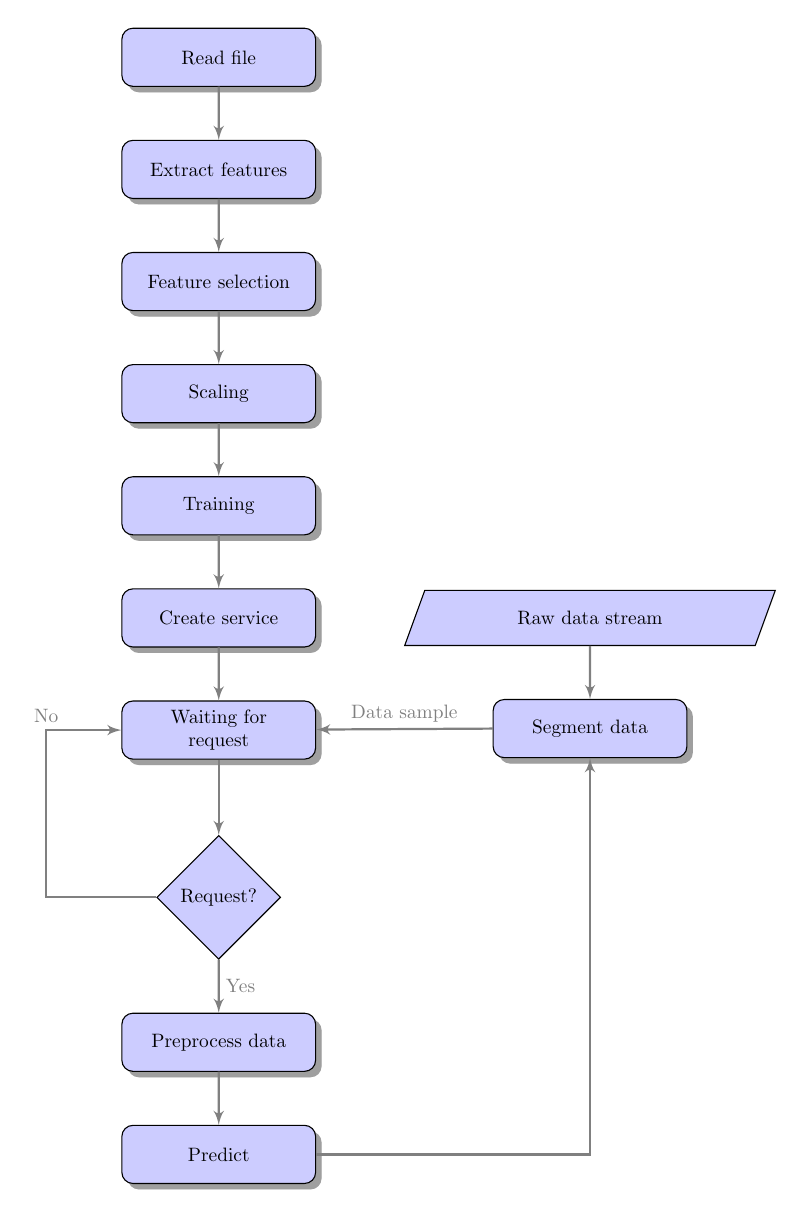
\begin{tikzpicture}[scale=0.7,transform shape]
		
		% Draw diagram elements
		%  \path \io{1}{Raw data};
		\path \etape{1}{Read file};
		%  \path (p1.south)+(0,-1.5) \etape{2}{Extract steps};
		\path (p1.south)+(0.0,-1.5) \etape{2}{Extract features};
		\path (p2.south)+(0.0,-1.5) \etape{3}{Feature selection};
		
		\path (p3.south)+(0.0,-1.5) \etape{4}{Scaling};
		\path (p4.south)+(0.0,-1.5) \etape{12}{Training};
		
		\path (p12.south)+(0,-1.5) \etape{5}{Create service};
		\path (p5.south)+(0,-1.5) \etape{6}{Waiting for request};
		\path (p6.south)+(0,-2.5) \dec{7}{Request?};
		\path (p7.south)+(0,-1.5) \etape{8}{Preprocess data};
		\path (p8.south)+(0,-1.5) \etape{9}{Predict};
		
		
		%\path (request?.south)+(0,-1.5) \etape{7}{Predicted};
		
		\path (p5.west)+(8.5,0) \io{10}{Raw data stream};
		\path (p10.south)+(0,-1.5) \etape{11}{Segment data};
		
		
		
		
		
		% Draw arrows between elements
		\path [line] (p1.south) -- node [above]{} (p2);
		\path [line] (p2.south) -- node [above]{} (p3);
		\path [line] (p3.south) -- node [above]{} (p4);
		\path [line] (p4.south) -- node [above]{} (p12);
		\path [line] (p12.south) -- node [above]{} (p5);
		\path [line] (p5.south) -- node [above]{} (p6);
		\path [line] (p6.south) -- node [above]{} (p7);
		\path [line] (p7.south) -- node [right]{Yes} (p8);
		\path [line] (p7.west) -- ++(-2,0) |- node [above]{No} (p6);
		\path [line] (p8.south) -- node [above]{} (p9);
		\path [line] (p9.east) -| node [above]{} (p11);
		
		\path [line] (p10.south) -- node [above]{} (p11);
		\path [line] (p11.west) -- node [above]{Data sample} (p6);
		\end{tikzpicture}
	
		\caption[Real-time implementation]{Real-time implementation.} \label{fig:realtime}
	\end{figure}
	\FloatBarrier
	\clearpage

\subsection{Result and analysis} \label{sub:unseen}	
The following paragraphs present the results along with an analysis of each experiment, when the robot traverses through two different terrains in this order:
	\begin{enumerate}
	\item Floor to carpet
	\item Hard mat to floor
	\item Hard mat to soft mat
	\item Soft mat to hard mat
	\item Soft mat to carpet
\end{enumerate}
\newpage

\subsubsection{Floor to carpet}
The data stream when the robot traverses from floor to carpet is shown in figure \ref{fig:gulvet4teppegraf}, where the vertical line is the transition between the terrains, and table \ref{tab:Gulvet4teppe} shows probabilities for each terrain on each step. The overall accuracy of predicting correctly is 88.9\%. However, how certain the classifier is to predict correctly is under 78\%. The fifth step is the transition and as shown, there is some confusion between floor and carpet. It is also worth noticing that at the fourth step the carpet has almost the same probability as the floor with 56.4\% and 42.5\% respectively. The soft mat and hard mat have small probabilities in every step and is less likely to be predicted.
	
	\begin{figure}[h]
		\centering
		\includegraphics[width=\textwidth,height=\textheight,keepaspectratio]{Figures/Gulvet4Teppe2_line2}
		\caption[Data stream of the transition from floor to carpet]{Data stream of the robot traversing from floor to carpet. The thick gray horizontal line is the boundary between the two terrains.}
		\label{fig:gulvet4teppegraf}
	\end{figure}
	
	
	\begin{table}[h]
		\centering
		\resizebox{\textwidth}{!}{%
			\begin{tabular}{@{}llllllllll@{}}
				\toprule
				\rowcolor[HTML]{FFFFC7} 
				\textbf{Step} & \textbf{1} & \textbf{2} & \textbf{3} & \textbf{4} & \textbf{5} & \textbf{6} & \textbf{7} & \textbf{8} & \textbf{9} \\ \midrule
				Floor & \cellcolor[HTML]{34FF34}0.782 & \cellcolor[HTML]{34FF34}0.680 & \cellcolor[HTML]{34FF34}0.747 & \cellcolor[HTML]{34FF34}0.561 & \cellcolor[HTML]{FD6864}0.564 & 0.282 & 0.206 & 0.252 & 0.282 \\
				Carpet & 0.105 & 0.289 & 0.162 & 0.425 & \cellcolor[HTML]{F8FF00}0.353 & \cellcolor[HTML]{34FF34}0.704 & \cellcolor[HTML]{34FF34}0.730 & \cellcolor[HTML]{34FF34}0.573 & \cellcolor[HTML]{34FF34}0.599 \\
				Soft mat & 0.008 & 0.009 & 0.010 & 0.008 & 0.010 & 0.005 & 0.009 & 0.009 & 0.015 \\
				Hard mat & 0.104 & 0.022 & 0.081 & 0.007 & 0.073 & 0.010 & 0.055 & 0.166 & 0.104 \\ \bottomrule
			\end{tabular}%
		}
		\caption[Results of transistion from floor to carpet]{Estimated probability of each terrain per step from floor to carpet. Values are marked green to represent correct predictions. For incorrect predictions, the actual value is marked yellow while the predicted value is marked red.}
		\label{tab:Gulvet4teppe}
	\end{table}
	\FloatBarrier
	\clearpage
	
\subsubsection{Hard mat to floor} \label{subsec:hmf}
The data stream when the robot traverses from hard mat to floor is shown in figure \ref{fig:mb3Gulvet}, where the vertical line is the transition between the terrains, and table \ref{tab:mb3Gulvet} shows probabilities for each terrain on each step. The overall accuracy of predicting correctly is 50\%. The first two steps have shown a high accuracy of predicting correctly with over 90\%. The third step, on other hand, which is the step before the transition, has a lower probability of the hard mat, with a similar probability as the carpet. It is also worth noticing that the force in the y-direction at this step differs from earlier steps. The fourth step is the transition, and is also where the model misclassifies the new terrain. It rather predicts it as carpet than floor.
		
\begin{figure}[h]
	\centering
	\includegraphics[width=\textwidth,height=\textheight,keepaspectratio]{Figures/MB3_3_Gulvet_line2}
	\caption[Data stream of the transition from hard mat to floor]{Data stream of the robot traversing from hard mat to floor. The thick gray horizontal line is the boundary between the two terrains.}
	\label{fig:mb3Gulvet}
\end{figure}
	
	
\begin{table}[h]
	\centering
	\resizebox{\textwidth}{!}{%
		\begin{tabular}{@{}lllllll@{}}
			\toprule
			\rowcolor[HTML]{FFFFC7} 
			\textbf{Step} & \textbf{1} & \textbf{2} & \textbf{3} & \textbf{4} & \textbf{5} & \textbf{6} \\ \midrule
			Floor & 0.006 & 0.008 & 0.172 & \cellcolor[HTML]{F8FF00}0.263 & \cellcolor[HTML]{F8FF00}0.141 & \cellcolor[HTML]{F8FF00}0.078 \\
			Carpet & 0.008 & 0.073 & 0.375 & \cellcolor[HTML]{FD6864}0.641 & \cellcolor[HTML]{FD6864}0.615 & \cellcolor[HTML]{FD6864}0.822 \\
			Soft mat & 0.006 & 0.004 & 0.008 & 0.023 & 0.019 & 0.014 \\
			Hard mat & \cellcolor[HTML]{34FF34}0.980 & \cellcolor[HTML]{34FF34}0.915 & \cellcolor[HTML]{34FF34}0.444 & 0.073 & 0.225 & 0.085 \\ \bottomrule
			\end{tabular}%
	}
	\caption[Results of transistion from hard mat to floor]{Estimated probability of each terrain per step walking from hard mat to floor. Values are marked green to represent correct predictions. For incorrect predictions, the actual value is marked yellow while the predicted value is marked red.}
	\label{tab:mb3Gulvet}
\end{table}
\FloatBarrier
\clearpage

\subsubsection{Hard mat to soft mat} \label{sec:hmssm}
 The data stream when the robot traverses from hard mat to soft mat is shown in figure \ref{fig:hardmatSoftMat} and table \ref{hardmatSoftMat} shows probabilities for each terrain on each step. The overall accuracy of predicting correctly is 100\%, while the average of choosing the correct terrain is 72.7\%. The forces in the y- and z-directions are much higher when walking on hard mat than soft mat. There is some uncertainty on the first, third and sixth step, where the probability of predicting correctly is less than 54\%.


	
	
	\begin{figure}[h]
		\centering
		\includegraphics[width=\textwidth,height=\textheight,keepaspectratio]{Figures/MB3MM_line2}
		\caption[Data stream of the transition from hard mat to soft mat.]{Data stream of the robot traversing from hard mat to soft mat. The thick gray horizontal line is the boundary between the two terrains.}
		\label{fig:hardmatSoftMat}
	\end{figure}
	
	\begin{table}[h]
		\centering
		\resizebox{\textwidth}{!}{%
			\begin{tabular}{@{}lllllllll@{}}
				\toprule
				\rowcolor[HTML]{FFFFC7} 
				\textbf{Step} & \textbf{1} & \textbf{2} & \textbf{3} & \textbf{4} & \textbf{5} & \textbf{6} & 7 & 8 \\ \midrule
				Floor & 0.329 & 0.015 & 0.081 & 0.059 & 0.022 & 0.115 & 0.059 & 0.048 \\
				Carpet & 0.105 & 0.045 & 0.105 & 0.041 & 0.015 & 0.095 & 0.037 & 0.033 \\
				Soft mat & 0.023 & 0.006 & 0.284 & \cellcolor[HTML]{34FF34}0.759 & \cellcolor[HTML]{34FF34}0.923 & \cellcolor[HTML]{34FF34}0.477 & \cellcolor[HTML]{34FF34}0.816 & \cellcolor[HTML]{34FF34}0.834 \\
				Hard mat & \cellcolor[HTML]{34FF34}0.542 & \cellcolor[HTML]{34FF34}0.935 & \cellcolor[HTML]{34FF34}0.529 & 0.142 & 0.040 & 0.313 & 0.088 & 0.085 \\ \bottomrule
			\end{tabular}%
		}
		\caption[Results of transistion from hard mat to floor]{Estimated probability of each terrain per step walking from hard mat to soft mat. Values are marked green to represent correct predictions. For incorrect predictions, the actual value is marked yellow while the predicted value is marked red.}
		\label{hardmatSoftMat}
	\end{table}
	\FloatBarrier
	\clearpage
	
\subsubsection{Soft mat to hard mat}
The data stream when the robot traverses from soft mat to hard mat is shown in figure \ref{fig:MM_4_Resten_BGraf}, and table \ref{MM4MB} shows probabilities for each terrain on each step. The overall accuracy of predicting correctly is 100\%, while the average of choosing the correct terrain is 79\%. Again, the forces in the y-, and z-directions are much higher when walking on hard mat than soft mat. There is some uncertainty on the first and fourth steps, where the probability of predicting correctly is less than 53.5\%.

	\begin{figure}[h]
		\centering
		\includegraphics[width=\textwidth,height=\textheight,keepaspectratio]{Figures/MM_4Resten_MB_line2}
		\caption[Data stream of the transition from soft mat to hard mat]{Figure showing data stream from sensor when the robot walked from soft mat to hard mat. The thick gray horizontal line is the boundary between the two terrains.}
		\label{fig:MM_4_Resten_BGraf}
	\end{figure}
	
	\begin{table}[h]
		\centering
		\resizebox{\textwidth}{!}{%
			\begin{tabular}{@{}llllllll@{}}
				\toprule
				\rowcolor[HTML]{FFFFC7} 
				\textbf{Step} & \textbf{1} & \textbf{2} & \textbf{3} & \textbf{4} & \textbf{5} & \textbf{6} & 7 \\ \midrule
				Floor & 0.099 & 0.019 & 0.018 & 0.138 & 0.021 & 0.008 & 0.038 \\
				Carpet & 0.065 & 0.023 & 0.017 & 0.134 & 0.050 & 0.005 & 0.022 \\
				Soft mat & \cellcolor[HTML]{34FF34}0.535 & \cellcolor[HTML]{34FF34}0.871 & \cellcolor[HTML]{34FF34}0.911 & \cellcolor[HTML]{34FF34}0.384 & 0.009 & 0.009 & 0.011 \\
				Hard mat & 0.300 & 0.086 & 0.054 & 0.344 & \cellcolor[HTML]{34FF34}0.921 & \cellcolor[HTML]{34FF34}0.978 & \cellcolor[HTML]{34FF34}0.930 \\ \bottomrule
			\end{tabular}%
		}
		\caption[Results of transistion from soft mat to hard mat]{Estimated probability of each terrain per step walking from soft mat to hard mat.Values are marked green to represent correct predictions. For incorrect predictions, the actual value is marked yellow while the predicted value is marked red.}
		\label{MM4MB}
	\end{table}
	\FloatBarrier
	\clearpage
\subsubsection{Soft mat to carpet}
The data stream when the robot traverses from soft mat to carpet is shown in figure \ref{fig:softcarpet}, and table \ref{tab:softcarpet} shows probabilities for each terrain on each step. The overall accuracy of predicting correctly is 87.5\%. Again, the forces in the y- and z-directions are much higher when walking on carpet than soft mat. There is some uncertainty on the first and fourth steps, where the probability of predicting correctly is less than 53.5\%. The fifth step is when the robot is on the new terrain, and has a probability of predicting it correct of 66.7\%. Regarding step six, the classifier makes a wrong prediction between carpet and hard mat with a probability of 93.3\%.
	
	
	\begin{figure}[h]
		\centering
		\includegraphics[width=\textwidth,height=\textheight,keepaspectratio]{Figures/MM4Teppe2_line2}
		\caption[Data stream of the transition from soft mat to carpet.]{Data stream of the robot traversing from soft mat to carpet. The thick gray horizontal line is the boundary between the two terrains.}
		\label{fig:softcarpet}
	\end{figure}
	
	\begin{table}[h]
		\centering
		\resizebox{\textwidth}{!}{%
			\begin{tabular}{@{}lllllllll@{}}
				\toprule
				\rowcolor[HTML]{FFFFC7} 
				\textbf{Step} & \textbf{1} & \textbf{2} & \textbf{3} & \textbf{4} & \textbf{5} & \textbf{6} & 7 & 8 \\ \midrule
				Floor & 0.021 & 0.022 & 0.068 & 0.031 & 0.100 & 0.020 & 0.016 & 0.018 \\
				Carpet & 0.017 & 0.019 & 0.049 & 0.023 & \cellcolor[HTML]{34FF34}0.667 & \cellcolor[HTML]{F8FF00}0.041 & \cellcolor[HTML]{34FF34}0.942 & \cellcolor[HTML]{34FF34}0.904 \\
				Soft mat & \cellcolor[HTML]{34FF34}0.909 & \cellcolor[HTML]{34FF34}0.914 & \cellcolor[HTML]{34FF34}0.762 & \cellcolor[HTML]{34FF34}0.891 & 0.017 & 0.007 & 0.006 & 0.006 \\
				Hard mat & 0.054 & 0.045 & 0.121 & 0.055 & 0.216 & \cellcolor[HTML]{FD6864}0.933 & 0.037 & 0.072 \\ \bottomrule
			\end{tabular}%
		}
		\caption[Results of transistion from soft mat to carpet]{Estimated probability of each terrain per step walking from soft mat to carpet.Values are marked green to represent correct predictions. For incorrect predictions, the actual value is marked yellow while the predicted value is marked red.}
		\label{tab:softcarpet}
	\end{table}
	\FloatBarrier
\newpage

\subsection{Summary}
A more realistic practical scenario is investigated. Five different setups where the robot walks between two different terrains achieved an overall accuracy of 85.3\%. It is worth noting that the robot often did not have a straight walk, which is also some of the reason why the step in each experiment varies. 
\\
\\
A common characteristic is that the probability decreases, particularly on the steps between the transition of terrain. Another characteristic is that the first and last step also tend to have a lower accuracy. Regarding the data provided from the sensor, the soft mat has a smaller force in the y- and z-directions than the other terrains. There is also no misclassification of the soft mat. However, there is some misclassification between floor and carpet, and hard mat and carpet.

\newpage
\section{Prediction on other sensor}
All previous experiments have only used data provided from the sensor mounted on the front left foot of the robot. Thus, it will be interesting to investigate the possibility of using the current training set to predict the data provided from a sensor mounted on the front right foot. The reason for testing the front right foot is that it has a more similar leg motion to the front left foot. The back foot, on the other hand, has a different leg motion which provides different data in each direction. In this following experiment, 30 data samples from the right foot for each terrain will be stored into a file and used to test the prediction. The model used is still SVM with feature set five.

	
\subsection{Results} 
Table \ref{tab:pred} shows the results of using the training set provided from left front foot to predict data from right front foot.
\begin{table}[h]
	\centering
	\begin{tabular}{lllll}
		\hline
		\textbf{Terrain} & \textbf{Floor} & \textbf{Carpet} & \textbf{Soft mat} & \textbf{Hard mat} \\ \hline
		\textbf{Floor} & \cellcolor[HTML]{FFFFC7}29 & 1 & 0 & 0 \\
		\textbf{Carpet} & 3 & \cellcolor[HTML]{FFFFC7}27 & 0 & 0 \\
		\textbf{Soft mat} & 0 & 0 & \cellcolor[HTML]{FFFFC7}30 & 0 \\
		\textbf{Hard mat} & 2 & 13 & 0 & \cellcolor[HTML]{FFFFC7}16 \\ \hline
		\textbf{Precision} & 96.7\% & 90\% & 100\% & 53.3\% \\
		\textbf{Recall} & 85.3\% & 65.9\% & 100\% & 100\% \\
		\textbf{F-score} & 90.6\% & 76.1\% & 100\% & 69.5\% \\ \hline
		\textbf{Accuracy} & \multicolumn{4}{c}{84.3\%} \\ \hline
	\end{tabular}
	\caption[Results of predicting sensor mounted on the front right foot]{Results of predicting on the sensor mounted on the front right foot.}
	\label{tab:pred}
\end{table}
	\FloatBarrier
	
\subsection{Analysis} 	
The overall accuracy of predicting data from the sensor mounted on the right foot is 84.3\%. It has a precision of over 90\% when predicting floor, carpet, and  soft mat. Hard mat, on the other hand, achieved only a precision of 53.3\%. The low precision is due to its tendency to be predicted as carpet. Results achieved in this experiment are similar to earlier experiments as in section \ref{sub:unseen}, when testing the classifier on new data samples. 
\\
\\
A further analysis will be looking at the data provided from each sensor on each terrain. Thus a mean of 10 steps on each terrain with each sensor is shown in figure \ref{fig:s1all}. The force in the x-direction between the two sensors differs from each other in every terrain. Meanwhile, the forces in the y- and and z-directions have similar values, except for the soft mat, where the force provided from the right front foot is much higher.

\begin{figure} [h]
	\centering
	\begin{subfigure}[b]{\textwidth}
			\includegraphics[width=\textwidth,height=\textheight,keepaspectratio]{Figures/s1gulv2}
			\caption{Floor}
			\label{fig:s1gulv2} 
		\end{subfigure}
		
		\begin{subfigure}[b]{\textwidth}
			\includegraphics[width=\textwidth,height=\textheight,keepaspectratio]{Figures/s1teppe}
			\caption{Carpet}
			\label{fig:s1teppe}
		\end{subfigure}
				\end{figure}
	\begin{figure}[h] \ContinuedFloat
	
		\begin{subfigure}[h]{\textwidth}\ContinuedFloat
			\includegraphics[width=\textwidth,height=\textheight,keepaspectratio]{Figures/s1hardmatte}
			\caption{Hard mat}
			\label{fig:s1hardmatte}
		\end{subfigure}
		
		\begin{subfigure}[b]{\textwidth}
			\includegraphics[width=\textwidth,height=\textheight,keepaspectratio]{Figures/s1mykmatte}
			\caption{Soft mat}
			\label{fig:s1mykmatte}
		\end{subfigure}
		\caption[Comparision between data stream sensor mounted on left and right front foot of the robot]{Comparison between data stream with the sensor mounted on the left and on the right front foot, on floor \ref{fig:s1gulv2}, carpet \ref{fig:s1teppe}, hard mat \ref{fig:s1hardmatte}, and soft mat	\ref{fig:s1mykmatte}.}
		\label{fig:s1all}
	\end{figure}	
	\FloatBarrier



\chapter{Discussion}
%Classification rate
\section{Classifiers performance}
Many classifiers have given a good performance; however, when the models were tested on new samples, the performance decreased, as seen in section \ref{seq:crossunseen}. The neural network and decision tree on raw sensor data did not give adequate performances. There is a high chance that these classifiers were overfitted and therefore not able to generalize the data well. It is also worth mentioning that the method of decimating the raw sensor data to a fixed length described in section \ref{subseq:FixLength} might also affect the performance. The method discards features at the start and the end of the feature vector because they were considered as less important. However, the longer the time series is, the more features are removed from the feature vector, with a risk of removing important features. The best performing classifier was the SVM with an overall accuracy of 94.8\%. Note that only SVM used the complete frequency domain as features, and therefore it is hard to tell whether it was the classifier or the feature set that achieved the high accuracy.  
\\
\\
Common characteristics are that the classifier tended to predict hard mat as carpet, and the soft mat in every trial achieved a high f-score as shown in section \ref{seq:crossunseen}. These common characteristics might be due to the sensor data as seen in figures \ref{fig:meanxyz} and \ref{fig:fftxyz}. Sensor data on hard mat and carpet have the most similar features and are most likely to be confused. While the sensor data on soft mat distinguishes from the other terrains, which is also the reason for a high f-score. Several feature selection methods were applied to remove common features and keep distinctive features. It is shown in table \ref{tab:exp2} that the RFE on feature set three did obtain minor improvement and achieved an accuracy of 97\%. It indicates that good features are kept and it is able to distinguish between each terrain, although there is still difficulty predicting the hard mat. The issue of predicting hard mat can be seen in \ref{fig:wrapperset5}, where there are especially many similar features behind the first ten of the sequence in the x-,y-, and z-directions. A further improvement is to test different values on the RFE, by discarding more features and keeping more distinctive features.
	
\section{Hyperparameter-tuning}
The achieved parameters from the grid search did not show significant improvement on the performance for both SVM and the Neural Network. The SVM was already a well performing model, and is therefore difficult to find parameter values to obtain a better performance. Neural network, on the other hand, only searched for the number of neurons in one or two hidden layers, while there are many other settings which should be tested to achieve a more optimal classifier. 
\\
\\
Regarding having binary numbers as output for the neural network, there was a minor improvement of the model when representing terrain with two binary numbers. A reason could be that, instead of choosing the output with the highest score, it treats every output equally. That is, every neuron that meets its threshold will be taken into account. Representations with four binary numbers, on the other hand, consider a terrain as unknown when more than two neurons fire. Allowing unknown terrains in the model leads to a higher rate of misclassification. However, despite being able to identify unknown terrains, it may be suitable if the robot is exploring or detecting new terrains.


\section{Transition between terrains}
The result achieved in the transition between terrains in section \ref{sub:unseen} has given an overall accuracy for all trials of 86.8\%. The overall accuracy of transition from floor to carpet is 88.9\%, which indicates that the classifier is able to identify terrains even with minor differences in their properties. However, after the transition from hard mat to floor, the classifier is confused between floor and carpet, as seen in table \ref{sec:hmssm}. This confusion has been shown from an earlier experiment in table \ref{svmexp}, where the carpet tends to have a small misclassification as floor. It is also worth mentioning that the robot tends to not walk straight during the experiments, which might cause the confusion between the terrains. All of the training samples were obtained when the robot walked straight. Thus, there is a high chance of affecting the classification when the robot walks toward the right or left. 
\\
\\
Regarding estimated probability on the first step on the new terrain, one can observe that the estimated probabilities are typically low. These issues might come from the fact that all training samples were collected when the robot walked on a certain terrain. Preventing this can be done by gathering training samples where the robot traverses through different terrains. Another thing to be observed is the step in the beginning, where the estimated probability of correct terrain is also typically low. It might indicate that the first step has a particular behavior, as in the middle the robot got more stable. Thus, extracting more data from the first step may improve the result.
\\
\\
Regarding how fast the robot detects new terrain, when the two terrains have significant differences in their properties, such as floor and soft mat, it detects the new terrain quickly . Terrains with less difference in their properties may not be detected as fast. Results of the transition from floor to carpet in table \ref{tab:Gulvet4teppe} show that the classifier sensed the new terrain after the second step on the new terrain. Note that the experiments are mostly based on transitions with the soft mat, which only gives an indication of how fast it detects the terrains with high difference in their properties. Thus, to give a more reliable evaluation, more experiments on transitions between floor, carpet, and hard mat is necessary.
	
\section{Predicting on the other sensor}
The sensor data provided from the front right foot differs somewhat from the data from the front left foot, as seen in figure \ref{fig:s1all}. The differences may come from when mounting the sensor on the robot. There is a possibility that the axis from the sensor on the front left foot does not precisely point in the same direction as the sensor on the front right foot. Despite differences in sensor data, the results from table \ref{tab:pred} indicate that most of the terrains have been predicted correctly, but predicting the hard mat correctly is still challenging.  Thus, it is possible to use the training data from the front left foot on the front right foot when incorporating them, but to achieve a more reliable result, it is best to train each sensor independently.


\section{Compared to earlier work}
To give an overview of the thesis performance, a comparison with earlier work is shown in table \ref{table:compareEarly}. These approaches were all performed with local sensing and tested on unseen data. The thesis approach has among the top performers and obtains similar result as in \cite{5752869,4059113,5602459,26b23e912c654fe4b7478fd910130195} with an accuracy of more than 90\%. Note that the experiments in \cite{5752869,4059113} were performed by a wheeled robot, which more easily achieves maintained stability and less noisy data when preprocessing data from a sensor than a legged robot. The thesis approach also outperforms past work which utilized more than one sensor \cite{6849778,6386243}. The work in \cite{26b23e912c654fe4b7478fd910130195} only utilized the servo and demonstrated an accuracy of 97\%.  However, the authors were incorporating all six servos from each leg which produces more sensor data to be preprocessed. It is also worth mentioning the work achieved higher accuracy when rocks and mulch were considered as one terrain. Utilizing more sensors or incorporating all four sensors in this work might also improve the results. The most similar comparison is with work reported in \cite{6784609}, where a similar quadruped robot and tactile sensor were used in the experiments. However, the work does not report the type of tactile sensor used, which makes it difficult to compare the sensor type itself. The experiments were tested on blue foil, styrofoam, linoleum, cardboard, and rubber, which have significant differences in their properties and achieved an accuracy of 84.69\%. As the robot in this thesis is able to distinguish between floor, carpet, and hard mat, it should also be able to predict all of those as well.

%26b23e912c654fe4b7478fd910130195

	\begin{table}[h]
		\centering
		\resizebox{\textwidth}{!} \\
				&  &  &  &  \\
				&  &  &  &  \\
				\multirow{2}{*}{Walas \cite{walastactile}} & \multirow{2}{*}{Tactile sensor} & \multirow{2}{*}{Linear Discriminant Analysis} & \multirow{2}{*}{5} & \multirow{2}{*}{76.67\%} \\
				&  &  &  &  \\
				\multirow{3}{*}{Kim el at. \cite{5602459}} & \multirow{3}{*}{\begin{tabular}[c]{@{}l@{}}Ground reaction force \\ Torque sensors\end{tabular}} & \multirow{3}{*}{SVM} & \multirow{3}{*}{4} & \multirow{3}{*}{78.75\%} \\
				&  &  &  &  \\
				&  &  &  &  \\
				\multirow{2}{*}{\textbf{Degrave el at. \cite{6784609}}} & \multirow{2}{*}{\textbf{Tactile sensor}} & \multirow{2}{*}{\textbf{Reservoir Computing}} & \multirow{2}{*}{\textbf{5}} & \multirow{2}{*}{\textbf{84.69\%}} \\
				&  &  &  &  \\
				\multirow{3}{*}{Kertész \cite{6849778}} & \multirow{3}{*}{\begin{tabular}[c]{@{}l@{}}Accelerometer\\ Paw sensor\end{tabular}} & \multirow{3}{*}{Naive Bayes} & \multirow{3}{*}{5} & \multirow{3}{*}{90.9\%} \\
				&  &  &  &  \\
				&  &  &  &  \\
				&  &  &  &  \\
				\multirow{3}{*}{Bermudez el at. \cite{6386243}} & \multirow{3}{*}{\begin{tabular}[c]{@{}l@{}}
					Vibration \\  motor	control data \\magnetic encoders
					\end{tabular}} & \multirow{3}{*}{SVM} & \multirow{3}{*}{3} & \multirow{3}{*}{93.8\%} \\
				&  &  &  &  \\
				&  &  &  &  \\
				&  &  &  &  \\
				\multirow{2}{*}{Giguere and Dudek \cite{5752869}} & \multirow{2}{*}{Tactile probe} & \multirow{2}{*}{Neural network} & \multirow{2}{*}{10} & \multirow{2}{*}{94.3\%} \\
				&  &  &  &  \\
%				\multirow{2}{*}{Stejskal el at. \cite{7487544}} & \multirow{2}{*}{Servos} & \multirow{2}{*}{SVM} & \multirow{2}{*}{10} & \multirow{2}{*}{96.2\%} \\
%				&  &  &  &  \\
				\multirow{2}{*}{Best el at. \cite{26b23e912c654fe4b7478fd910130195}} & \multirow{2}{*}{Servos} & \multirow{2}{*}{SVM} & \multirow{2}{*}{4} & \multirow{2}{*}{97.3\%} \\
				&  &  &  &  \\
				\multirow{2}{*}{Thesis approach} & \multirow{2}{*}{Optical tactile sensor} & \multirow{2}{*}{SVM} & \multirow{2}{*}{4} & \multirow{2}{*}{94.8\%} \\
				&  &  &  &  \\ \bottomrule
			\end{tabular}%
		}
		\caption[Comparision between thesis approach and earlier approches]{Comparison between thesis approach with other approaches on unseen data. Thesis result is the mean of the accuracy from LOOCV on unseen data from the best performed classifier obtained in section \ref{sb:svmwrapper}. The most similar approach with robot platform and sensor used is marked with bold text.}
		\label{table:compareEarly}
	\end{table}
	\FloatBarrier
	

	
\section{Conclusion}
The aim of this thesis was to investigate the possibility of terrain classification using a 3D optical force sensor. The approach was machine learning on force data provided from the sensor mounted on a quadruped robot. Four different terrains - floor, carpet, hard mat, and soft mat - were used in the experiments. The data set consisted of the robot walking on each terrain separately. Although the terrains such as the floor, carpet, and hard mat have similar properties, analysis of the sensor data showed that the sensor is able to perceive small significant differences between them. The differences can be found in the sensor data in the y- and z-directions, where the amount of force and the shape of time series differ between each terrain. Sensor data in the x-direction, on the other hand, provided almost identical features from the floor, carpet, and hard mat.
\\
\\
The evaluation of the force sensor was done by using five different classifiers - naive Bayes, decision tree, KNN, neural network, and SVM - with five different feature sets. The feature sets consist of either using decimated raw data in the time domain or frequency domain, or statistical features in the time domain, frequency domain or both. Many of the classifiers obtained a high accuracy during the cross validation. However, when selecting five well-performing models on unseen data, the accuracy dropped as anticipated. The neural network and decision tree, which had an accuracy of over 90\%, decreased to 64\% and 78\% respectively. This may indicate that the models were overfitted and did not generalize data well. The combination of selected features from the complete frequency domain and SVM gave the best results with an accuracy of 94.8\%. This feature set seems to contain distinctive and informative features that make the terrains distinguishable. However, the model still had difficulty predicting the hard mat. 
\\
\\
A real-time implementation was implemented in order for the purpose of a more realistic scenario when the robot was walking through different terrains. The real-time implementation was able to segment sensor data and make the classification fast. However, since the algorithm was only tested on a certain gait and flat surfaces, one might achieve a different performance when another gait or more rough terrain is chosen. The experiment showed a feasible result with an overall accuracy of 86.8\%. Note that there were some trials where the robot did not have straight locomotion, which might have decreased the performance
\\
\\
The last experiment demonstrated the possibility of using training data from a sensor mounted on the front left foot to predict front right foot data samples. The data provided from both sensors showed a significant difference but had some of the same shapes of the time series. The results of this experiment indicate that one can obtain more training samples by using sensor data from both sensors. However, in case the legs have different walking behaviors, it may be more appropriate to have separate training samples for each sensor. 
\\
\\
The results confirm that the optical force sensor is suitable to use for terrain classification. Comparing the results obtained from cross-validation on unseen data from earlier studies, the thesis approach has achieved among the top performances with an accuracy of 94.8\% on SVM. Note that this work only utilized one sensor on a legged robot to discriminate the terrains, while much of the other past work have either used sensor fusion or wheeled robots, which provide more stable locomotion to achieve a good result. As the sensor in this thesis is able to distinguish terrains such as floor, carpet, and hard mat, which have similar properties, there is a high chance of it correctly predicting outdoor terrains as well.
	
\section{Future work}
The classifier is based on the features from the sensor data. However, features of the terrain itself such as hardness and friction are not analyzed directly, which can be addressed in future work. 
\\
\\
This thesis has only experimented with flat terrains. It will be interesting to include rougher surfaces or other types and investigate the performance with the current model. 
\\
\\
This thesis has mostly used sensor data from one leg. However, incorporating all four legs might increase the performance of terrain classification. 
\\
\\
Many authors have utilized sensor fusion to achieve feasible results. Thus, using data from other sensors such as leg motion, servos etc. could further aid the performance.
\\
\\
Instead of explicitly labeling the terrain, having unsupervised learning could be appropriate. This gives the robot the ability to explore and detect terrains by itself.
\\
\\
Only one robot was used to evaluate the sensor. However, different platforms may not give the same results. Thus, different robot platforms should be tested to achieve a more reliable evaluation of the sensor.
\\
\\
One of the important abilities for a robot to achieve terrain classification is to change their gaits on different terrains. Thus, the approach can be further extended to give the robot the ability to select appropriate gaits between different terrains.

%http://www2.ift.ulaval.ca/~pgiguere/terrainID.html
%Optical force (Legged Robots)
%https://link.springer.com/referenceworkentry/10.1007/978-3-540-30301-5_17
	
%An Overview of Legged Robots


\backmatter{}
\addcontentsline{toc}{chapter}{Bibliography}
\bibliography{bib}
\bibliographystyle{ieeetr}

\part*{Appendices} 
\addcontentsline{toc}{chapter}{Appendices}
\appendix
\chapter{Code of segmentation of data} \label{ap:code}
The custom method of segmenting desired data from the sensor is in listing \ref{ap:code1}. The code only for one sensor.
\lstinputlisting[language=C++, caption={A simplified method to achieve a fixed length of data sequence},captionpos=b,label={ap:code1},frame=single,breaklines=true]{code/data_seg.cpp}

\begin{comment}
\chapter{SVM kernels} \label{ap:kernel}
The SVM kernels reflect how the similarity between two datapoint is computed. There are three commonly used kernel functions, shown in table \ref{aptab:kern}. Even there are some theory how to chose the kernel, but generally is found by experiment with different values and use that works best. Regarding the gamma value that will be grid search in section \ref{pa:svmp}, only RBF will be affected by the gamme value.

\begin{table}[h]
	\centering
	\begin{tabular}{ll}
		\hline
		\textbf{Kernel name} & \textbf{Values} \\ \hline
		\multirow{2}{*}{Linear} & \multirow{2}{*}{$\vec{x} \cdot \vec{x}$} \\
		&  \\
		\multirow{2}{*}{RBF} & \multirow{2}{*}{$exp(-\gamma\vert\vert \vec{x}\cdot\vec{y}\vert\vert^{2})$} \\
		&  \\
		Polynomial & $(1 + \vec{x} \cdot \vec{y})^{d}$  \\ \hline
	\end{tabular}
	\caption{Table shows the Pythons SVM kernels.}
	\label{aptab:kern}
\end{table}
\FloatBarrier
\end{comment}

\chapter{Selected features} \label{ap:self}
The following paragraphs shows different features selected from both method removing features with low variance and recursive feature elimination.

\subsubsection{Set 1}
Filter
\begin{align}
f_{set1} &= \left\{x_{8}, x_{19},\dotsc, x_{24}, x_{27},  x_{53}, \dotsc, x_{61}, x_{80}, \dotsc, x_{83}\right.\nonumber\\
&\qquad \left.{}  x_{86},\dotsc,x_{119} \right.\nonumber\\
&\qquad \left.{}  y_{14},\dotsc,  y_{27}, y_{52}, \dotsc, y_{60}, y_{81},\dotsc, y_{84}, y_{101}, \dotsc, y_{123} \right.\nonumber\\
&\qquad \left.{} z_{1},\dotsc,z_{125} \right\}
\end{align}

Wrapper
\begin{align}
f_{set1} &= \left\{x_{1}, x_{5}, x_{6}, x_{9}, x_{12}, x_{13}, x_{14}, x_{19},x_{20},x_{23},x_{25},x_{26},  \right.\nonumber\\
&\qquad \left.{}  x_{35}, x_{39},x_{45},x_{47},x_{50},x_{51},x_{52},x_{55},x_{56},x_{60},x_{62},x_{64},x_{65},x_{66}, \right.\nonumber\\
&\qquad \left.{}  x_{72},x_{73},x_{74},x_{76},x_{80},x_{81},x_{84},x_{88},x_{91},x_{93},x_{94},x_{97},x_{98},x_{103}, \right.\nonumber\\
&\qquad \left.{}  x_{105},x_{107},x_{108},x_{109},x_{111},x_{113},x_{114},x_{116},x_{118},x_{119},x_{120},x_{123},x_{124},x_{125}, \right.\nonumber\\
&\qquad \left.{}  y_{1},y_{2},y_{3},y_{6},y_{9},\dotsc,y_{13},y_{16}, y_{17},y_{26},\dotsc,y_{30},y_{33}, y_{34},y_{37},\dotsc,y_{40}, \right.\nonumber\\
&\qquad \left.{}  y_{42}, y_{44}, y_{47},\dotsc, y_{52}, y_{54}, y_{57},\dotsc, y_{60}, y_{63}, y_{65}, y_{66}, y_{67}, y_{69}, \right.\nonumber\\
&\qquad \left.{}  y_{70}, y_{71}, y_{73}, y_{74}, y_{76}, y_{77}, y_{78}, y_{81}, y_{83}, y_{85}, y_{86}, y_{89}, y_{91}, y_{94}, y_{97}, y_{98}, \right.\nonumber\\
&\qquad \left.{}  y_{101}, y_{102}, y_{103}, y_{105}, y_{106}, y_{109}, y_{110}, y_{114}, y_{116}, y_{118}, y_{121}, y_{122}, y_{124}, y_{125}, \right.\nonumber\\
&\qquad \left.{}  z_{2}, z_{3}, z_{4}, z_{6}, z_{9}, z_{10}, z_{11}, z_{13},z_{27},\dotsc,z_{30},z_{32}, z_{35}, z_{36}, z_{38}, z_{39}, z_{40}, \right.\nonumber\\
&\qquad \left.{}  z_{43}, z_{44}, z_{47}, z_{48}, z_{49}, z_{51}, z_{53}, z_{54}, z_{55}, z_{58}, z_{59}, z_{60}, z_{63}, z_{64}, z_{66}, z_{67}, z_{68}, \right.\nonumber\\
&\qquad \left.{}  z_{72},\dotsc , z_{75}, z_{78}, z_{79}, z_{81},\dotsc, z_{84}, z_{88}, z_{89}, z_{92}, z_{95}, \right.\nonumber\\
&\qquad \left.{} z_{100}, z_{103}, z_{106},\dotsc ,z_{109}, z_{115}, z_{116}, z_{119}, z_{120}, z_{121}, z_{122}, z_{125}\right\}
\end{align}


\subsubsection{Set 2}
\paragraph{Filter}
\begin{align}
f_{set2} &= \left\{x_{max}, x_{kurtosis}, x_{skew}, \right.\nonumber\\
&\qquad \left.{} y_{max}, \right.\nonumber\\
&\qquad \left.{} z_{min}, z_{max}, z_{mean}, z_{var} \right\}
\end{align}

\paragraph{Wrapper}
\begin{align}
f_{set2} &= \left\{x_{var}, x_{std}, \right.\nonumber\\
&\qquad \left.{} y_{max}, y_{kurtosis}, y_{skew}, y_{var}, \right.\nonumber\\
&\qquad \left.{} z_{max}, z_{kurtosis}, z_{var}, z_{std} \right\}
\end{align}


\subsubsection{Set 3}
\paragraph{Filter}
\begin{align}
f_{set3} &= \left\{x_{1}, z_{1} \right\}
\end{align}


\paragraph{Wrapper}
\begin{align}
f_{set3} &= \left\{x_{1},\dotsc,x_{8}, x_{10},x_{13},\dotsc,x_{19},x_{21},x_{22},x_{24},x_{27} \right.\nonumber\\
&\qquad \left.{}  x_{30},x_{32},x_{33},x_{34},x_{37},x_{38},x_{39}, \right.\nonumber\\
&\qquad \left.{}  y_{1},y_{3},y_{4},y_{6},\dotsc,y_{13},y_{15},y_{16},y_{20},y_{22},y_{24},y_{25}, \right.\nonumber\\
&\qquad \left.{} y_{27},y_{28},y_{29},y_{31},y_{32},y_{33},y_{36},y_{37},y_{38},y_{39},y_{51}, \right.\nonumber\\
&\qquad \left.{} z_{1},\dotsc,z_{11},z_{13},z_{17},\dotsc,z_{22},z_{24},z_{34},  \right.\nonumber\\
&\qquad \left.{} z_{36},z_{38},z_{39},z_{51},z_{59},z_{60},z_{61} \right\}
\end{align}



\subsubsection{Set 4}
\paragraph{Filter}
\begin{align}
f_{set4} &= \left\{fx_{max}, fx_{kurtosis}, fx_{skew}, fx_{E}, \right.\nonumber\\
&\qquad \left.{} fy_{max}, fy_{E}, \right.\nonumber\\
&\qquad \left.{} fz_{min}, fz_{max}, fz_{mean}, fz_{var}, fz_{E} \right\}
\end{align}

\paragraph{Wrapper}
\begin{align}
f_{set4} &= \left\{fx_{var}, fx_{std}, \right.\nonumber\\
&\qquad \left.{} fy_{max}, fy_{mean}, fy_{kurtosis}, fy_{skew}, fy_{std}, fy_{E}, \right.\nonumber\\
&\qquad \left.{} fz_{min}, fz_{max}, fz_{kurtosis}, fz_{var} \right\}
\end{align}

\subsubsection{Set 5}
\paragraph{Filter}
\begin{align}
f_{set5} &= \left\{x_{max}, x_{kurtosis}, x_{skew}, fx_{max}, fx_{kurtosis}, fx_{skew}, fx_{E}, \right.\nonumber\\
&\qquad \left.{} y_{max}, fy_{max}, fy_{E}, \right.\nonumber\\
&\qquad \left.{} z_{min}, z_{max}, z_{mean}, z_{var}, fz_{min}, fz_{max}, fz_{mean}, fz_{var}, fz_{E} \right\}
\end{align}

\paragraph{Wrapper}
\begin{align}
f_{set5} &= \left\{x_{var}, x_{std}, fx_{mean}, fx_{var}, fx_{std}, fx_{E}, \right.\nonumber\\
&\qquad \left.{} y_{skew}, fy_{max}, fy_{kurtosis}, fy_{skew}, fy_{E}, \right.\nonumber\\
&\qquad \left.{} z_{min}, z_{max}, z_{mean}, z_{kurtosis}, z_{var}, fz_{min}, fz_{max}, fz_{mean}, fz_{kurtosis} \right\}
\end{align}
%\chapter{Sensor datasheet}\label{ap:datasheet}
%\includepdf[pages=-]{Datasheet/Sensor.pdf}

\end{document}
